\documentclass[11pt,a4paper]{article}

% ---------------------------------------------------------------------------
% Packages
% ---------------------------------------------------------------------------
\usepackage[utf8]{inputenc}
\usepackage[T1]{fontenc}
\usepackage{lmodern}
\usepackage{amsmath,amssymb,amsthm}
\usepackage{stmaryrd}
\usepackage{graphicx}
\usepackage{tikz}
\usepackage{booktabs}
\usepackage{longtable}
\usepackage{array}
\usepackage{hyperref}
\usepackage{url}
\usepackage{listings}
\usepackage{xcolor}
\usepackage{microtype}
\usepackage{natbib}
\usepackage{enumitem}
\usepackage{calc}
\usepackage{multirow}
\usepackage{tabularx}

% Theorem environments
\theoremstyle{definition}
\newtheorem{definition}{Definition}[section]
\newtheorem{theorem}{Theorem}[section]
\newtheorem{coretheorem}{Theorem}
\newtheorem{corollary}{Corollary}[section]
\newtheorem{lemma}{Lemma}[section]
\newtheorem{proposition}{Proposition}[section]

\theoremstyle{remark}
\newtheorem{remark}{Remark}[section]

% Line length
\setlength{\textwidth}{6.5in}
\setlength{\oddsidemargin}{0in}
\setlength{\evensidemargin}{0in}
\setlength{\textheight}{9in}
\setlength{\topmargin}{-0.5in}

% Listings style
\lstset{
    basicstyle=\small\ttfamily,
    breaklines=true,
    frame=single,
    numbers=left,
    numberstyle=\tiny\color{gray},
    keywordstyle=\color{blue},
    commentstyle=\color{green!50!black},
    stringstyle=\color{red},
}

% Define Turtle language for listings (used in PROV-O examples)
\lstdefinelanguage{Turtle}{
    morekeywords={a,@prefix,@base,PREFIX,BASE,TRUE,FALSE},
    sensitive=false,
    morecomment=[l]{\#},
    morestring=[b]{"},
    morestring=[s]{<>},
}

% ---------------------------------------------------------------------------
% Title
% ---------------------------------------------------------------------------
\title{ADL Lite: An Event-First Capability-Lifecycle Registry for LLM Agent Ecosystems}

\author{
    Anonymous Authors \\
    \textit{Affiliation withheld for peer review}
}

\date{}

% ---------------------------------------------------------------------------
% Document
% ---------------------------------------------------------------------------
\begin{document}

\maketitle

\begin{abstract}
LLM agents are proliferating across enterprise and open ecosystems, each advertising tools, APIs, and knowledge-domain capabilities. Yet no lightweight, verifiable, lifecycle-aware registry exists to govern what a capability claims, how it evolves, and whether it remains trustworthy. Existing governance layers---KYA for permissions and AgentSafe for architecture-level oversight---leave this gap unaddressed. ADL Lite fills it as an event-first capability-lifecycle registry. Drawing on Wittgenstein's thesis that ``the world is the totality of facts, not of things,'' ADL Lite treats events---not objects---as the fundamental ontological primitive, while distinguishing occurrents (events as they occur) from their immutable records (EventChains). Capabilities are modeled as append-only, cryptographically linked EventChains, with all lifecycle state (status, confidence, validators) derived exclusively from event history through deterministic functions. Every capability claim, validation, deprecation, and fork is an auditable event; this design eliminates stored mutable state and the consistency defects it introduces.

We provide a two-level ontological analysis that situates ADL Lite within foundational ontologies (BFO, DOLCE, UFO), formalizes identity conditions and three forms of ontological dependence, and defines a decidable precondition language for lifecycle transitions. We further provide a complete formal semantics, together with seven proved properties including determinism, confluence under fork, and CRDT convergence.

We empirically validated the registry on 201 EventChains derived from the IBM Anti-Money Laundering dataset (9,300 events), confirming zero integrity failures and linear scalability under architectural stress tests. These findings are supplemented by concurrency stress tests, adversarial integrity trials, and comparative baselines against nanopublications and Git-native systems. This paper is positioned as a framework paper establishing the ontological and formal foundations of capability-lifecycle governance. The registry is implemented as a pip-installable Python toolkit operating on Markdown files in standard Git repositories, targeting lightweight deployment scenarios where full OWL/SPARQL infrastructure is unavailable or unnecessary.

\end{abstract}

\noindent\textbf{Keywords:}
agent audit; capability registry; lifecycle audit; event sourcing; multi-agent systems; provenance; operational ontology

\section{Introduction}\label{sec:introduction}
\subsection{Background: The Agent Capability Governance Gap}\label{subsec:background}

Large language model (LLM) agents are proliferating across ecosystems. Each agent exposes a set of \emph{capabilities}: tools, APIs, knowledge domains, and interaction protocols. A capability is a claim---``I can retrieve weather data,'' ``I can execute SQL,'' ``I can reason about financial risk''---that other agents and human operators must evaluate before delegation. But who records what a capability does, how it evolves, and whether it is trustworthy? Today, capability claims are scattered across README files, API documentation, and prompt templates. They are revised without audit trails, deprecated without ceremony, and forked without attribution. A lightweight, verifiable, lifecycle-aware registry of agent capabilities does not yet exist.

\paragraph{Existing governance layers.}
Three recent lines of work address adjacent aspects of agent governance, but none fills the capability-registry gap.

\textbf{KYA} (\emph{Know Your Agent}, arXiv:2605.25376) is a framework-agnostic trust layer for agent systems that provides a permissions model with HMAC-chained integrity \cite{kya2025}. It achieves approximately 1,800 operations per second and is available as the \texttt{veldt-kya} package on PyPI. KYA governs \emph{who} can invoke \emph{what}, but it does not govern the \emph{lifecycle} of a capability itself: there is no \texttt{VALIDATE} event that records an independent audit of a tool's behavior, no \texttt{DEPRECATE} event that marks a retired protocol, and no \texttt{FORK} event that traces a community derivative. KYA secures the permission boundary; it does not register the capability's provenance.

\textbf{AgentSafe} (arXiv:2512.03180) is a unified governance framework spanning design-time, runtime, and audit phases \cite{agentsafe2025}. It provides architecture-level governance---data-flow validation, policy enforcement, and safety guardrails---but it is heavyweight and requires integration with a service mesh or runtime orchestrator. It does not offer a lightweight, Markdown-native format that a single agent can author, cryptographically link, and commit to version control without enterprise infrastructure.

\textbf{LLM-native ontology engineering} (Talukdar et al., arXiv:2604.23090; LLM4ACOE) uses multi-agent LLM pipelines to generate OWL ontologies from natural-language requirements \cite{talukdar2025}. These systems produce static taxonomies and relation schemas, but they do not govern the \emph{runtime lifecycle} of the concepts they create: there is no event-sourced record of validation, deprecation, or fork, and no tamper-evident chain linking an agent's assertion to its subsequent revision or retirement. The ontology is produced, not governed.

Two additional bodies of work are complementary but distinct. \textbf{``From Agent Traces to Trust''} (arXiv:2606.04990) surveys provenance frameworks for agent systems and explicitly notes that ``a unified trace schema is still needed'' \cite{agenttraces2025}. ADL Lite is that schema: an event-first, cryptographically linked trace format in which every capability claim, validation, deprecation, and fork is a first-class auditable event. \textbf{SafeAgent} (arXiv:2604.17562) is a safety protocol for LLM agents that defines red-team evaluation procedures and harm-classification taxonomies \cite{safeagent2025}. It governs \emph{safety assessment}, not \emph{capability registration}; its concern is whether an agent is dangerous, not whether its advertised capabilities are authentic, current, and traceable.

\paragraph{Defining the gap.}
No existing system simultaneously satisfies four properties that define the capability-registry design space: (a)~document-native authoring in plain Markdown, (b)~built-in tamper detection through cryptographic hash chaining, (c)~lifecycle state machines with declarative preconditions, and (d)~pip-installable deployment requiring no enterprise infrastructure. KYA satisfies (b) and (d) but lacks (a) and (c). AgentSafe partially satisfies (c) but lacks (a), (b), and (d). LLM-native OE tools satisfy (a) in a limited sense (natural-language input) but lack (b), (c), and (d). The intersection of all four properties remains unoccupied.

\paragraph{Defining ``operational ontology.''}
We use the term \emph{operational ontology} in a specific sense that requires explicit definition, because the term carries distinct meanings in adjacent literatures. In the OBO Foundry ecosystem, an ``operational ontology'' typically means an application ontology deployed in a running bioinformatics pipeline (as opposed to a reference ontology) \cite{obo_foundry}. In programming-language theory, ``operational semantics'' defines the meaning of a program through its execution on an abstract machine. In knowledge-engineering practice, ``executable ontologies'' (e.g., UFO-B executable specifications \cite{guizzardi2024ufob}) are ontologies equipped with first-order logic axioms that can be evaluated by a reasoner. ADL Lite's usage differs from all three: we mean an ontology in which the \emph{operational semantics of lifecycle transitions}---preconditions, state derivation, and consensus rules---are co-located with the \emph{data structure} (EventChain) in a single lightweight package. In the present framing, the ``ontology'' is the set of capability concepts an agent ecosystem manages; the ``operational'' aspect is the fact that the same YAML-declared rules that define what can happen to a capability are enforced at append time by the ActionExecutor, without requiring an external workflow engine, OWL reasoner, or triple store. This co-location of governance semantics and data structure is the defining characteristic of ADL Lite's operational ontology.

\paragraph{Ontological novelty of the event-first stance.}
We emphasize that ADL Lite's contribution is not the philosophical thesis that ``events are fundamental''---a position already well-established by Wittgenstein's \emph{Tractatus} (\S1.1), BFO's \emph{occurrent}, DOLCE's \emph{perdurant}, and UFO-B's \emph{event} \cite{wittgenstein_tractatus,bfo,dolce,ufo}. Rather, ADL Lite's contribution is the \emph{operationalization} of this stance: the translation of an event-first philosophical commitment into a deployable, Markdown-native, cryptographically enhanced capability-lifecycle mechanism. In foundational ontologies, events and continuants are typically treated as co-equal top-level categories; ADL Lite treats events as the \emph{sole architectural primitive} from which all lifecycle state---status, confidence, validator identity---is derived through deterministic functions. This is an engineering reduction, not a metaphysical elimination: capabilities are not denied ontological standing, but their \emph{computable} properties (status, confidence) are made dependent on event history. This operationalization distinguishes ADL Lite from descriptive event ontologies (CIDOC CRM, SEM/LODE) that record what happened without enforcing what can happen. It also distinguishes ADL Lite from cryptographic provenance systems (nanopublications, PROV-O) that provide tamper detection without lifecycle state machines.

\paragraph{Why existing families are insufficient.}
We demonstrate systematic awareness by showing that representative systems from five distinct families fail to cover the full intersection of properties (a)--(d):

\textbf{Descriptive event ontologies (CIDOC CRM, SEO).} CIDOC CRM provides event-centric descriptive modeling and is widely deployed in cultural heritage \cite{cidoc_crm}. The Subject-Event Ontology (SEO) offers event-first patterns for web-scale data \cite{boldachev2025seo}. Both fail to satisfy (b) and (c): they record what happened without cryptographic integrity guarantees and without declarative preconditions for lifecycle state transitions. Moreover, production deployments typically require reasoning-enabled RDF/OWL toolchains, triple stores, and SPARQL endpoints, violating (d).

\textbf{Cryptographic provenance systems (PROV-O, nanopublications with Trusty URIs).} PROV-O provides a W3C-standard provenance vocabulary \cite{w3c_prov_o}; nanopublications with Trusty URIs achieve cryptographic integrity for atomic claims through hash-based URIs \cite{nanopublications,trusty_uris}. However, PROV-O lacks (b) natively: it describes provenance without built-in tamper detection, and it requires RDF tooling that conflicts with (a) and (d). Nanopublications satisfy (b) for atomic claims but lack (a) because they require RDF serialization and lack (c) because they provide no built-in lifecycle governance or state-machine preconditions.

\textbf{Markdown-native knowledge tools (Foam, Obsidian).} These tools satisfy (a) and (d) by design: they operate on plain Markdown files with minimal installation overhead \cite{foam2020,obsidian2024}. However, they provide neither (b) nor (c): they lack cryptographic hash chaining and provide no lifecycle state machines or precondition enforcement.

\textbf{Summary.} Each family lacks at least one property, and no family satisfies all four. ADL Lite occupies this intersection by integrating these properties into a coherent operational ontology, not by inventing any individual component.

\subsection{Research Gap: Capability Lifecycle Governance as Ontological Analysis}\label{subsec:research-gap}

The specific research gap addressed in this paper can be formulated as follows: \emph{How can an event-first capability registry achieve lifecycle traceability and multi-agent governance without requiring object-first mutable state, expert curation, or heavyweight tooling?} This gap has both an engineering dimension and an ontological dimension.

The \textbf{engineering dimension} concerns deployment friction. Existing operational ontology platforms require specialized expertise, dedicated infrastructure, and manual curation workflows that do not scale with the velocity of agent-generated capability artifacts \cite{hogan2021knowledge,guha2016schemaorg}. LLM-based agents cannot participate in capability registry construction because they lack programmatic access to the proprietary interfaces through which ontologies are constructed.

The \textbf{ontological dimension} concerns the status--history relationship. In an object-first registry, a capability's status is a property of the capability record. In an event-first registry, a capability's status is a derivative of its history. The transition from object-first to event-first is not merely a software design pattern (though it resembles event sourcing \cite{event_sourcing,cqrs}); it is an ontological reorientation that changes the fundamental categories of the registry. While event-centric modeling has been extensively analyzed in the applied ontology literature (CIDOC CRM, SEM, SEO, UFO-B), the \emph{operationalization} of event-first semantics---combining cryptographic integrity, deterministic lifecycle derivation, and declarative preconditions in a single lightweight system---has not been systematically studied.

This paper addresses both dimensions by presenting ADL Lite, an event-first operational ontology in which capabilities are modeled as append-only, cryptographically linked EventChains, and all lifecycle state is derived exclusively from event history. The paper's primary contribution is an \textbf{ontological analysis} that situates ADL Lite within the landscape of foundational ontologies (BFO, DOLCE, UFO), formalizes its categories and identity conditions, and proves key properties of its derivation semantics.

\subsection{Contributions}\label{subsec:contributions}

The contributions of this paper are organized around three axes: ontological analysis, formal semantics, and empirical validation.

\textbf{Contribution 1: Ontological analysis of event-first capability governance.} We analyze ADL Lite's core categories through the lens of three influential foundational ontologies:
\begin{itemize}[leftmargin=2em]
    \item We show that ADL Lite's \texttt{Event} corresponds to the BFO category of \emph{occurrent} and to the DOLCE category of \emph{perdurant}.
    \item We argue that ADL Lite's \texttt{Concept} (here, a capability definition) is best understood as a BFO \emph{generically dependent continuant} or as a DOLCE \emph{non-physical object}.
    \item We demonstrate that ADL Lite's L3 relations instantiate UFO \emph{relators} with event-based lifecycles.
    \item We formalize identity conditions for events, capabilities, and chains, and analyze three forms of ontological dependence (historical, generic, mutual).
\end{itemize}

\textbf{Contribution 2: Formal derivation semantics with proved properties.} We provide a complete formal foundation comprising:
\begin{itemize}[leftmargin=2em]
    \item An event alphabet $\Sigma = \Sigma_{\text{life}} \cup \Sigma_{\text{comm}}$ partitioned into lifecycle and communication events.
    \item A well-formedness predicate $\text{WF}(C)$ over EventChains.
    \item Status derivation $\delta(C)$ and confidence aggregation $\gamma(C)$ as deterministic functions.
    \item Fork and confluence semantics.
    \item Seven proved properties: determinism (Theorem~1), confluence under fork (Theorem~2), transition monotonicity (Theorem~3), confidence boundedness (Theorem~4), confidence monotonicity under independent validation (Theorem~5), status--confidence consistency (Theorem~6), and CRDT convergence (Theorem~7).
    \item An analysis of expressive power in relation to Event Calculus and Description Logic.
\end{itemize}

\textbf{Contribution 3: Empirical validation of formal semantics and ontological consistency.} We evaluate ADL Lite on 201 EventChains derived from the IBM Anti-Money Laundering (AML) HI-Small dataset (9,300 events), empirically validating the formal semantics against seven proved theorems from Contribution~2. The evaluation confirmed:
\begin{itemize}[leftmargin=2em]
    \item Zero integrity failures across all chains, including the longest chain (300 events).
    \item 100\% accuracy on 2,204 exhaustive status derivation test cases.
    \item Perfect precision and recall (P = R = F1 = 1.0) on 19 precondition enforcement test cases.
    \item Linear scalability: 20{,}955 events per second on modest hardware.
\end{itemize}
These results are not a domain-level evaluation of AML effectiveness; they validate that the event-first ontological architecture---including the deterministic derivation semantics, hash-linked integrity guarantees, and seven formally proved properties---is computationally feasible, cryptographically sound, and empirically correct. Domain-level evaluation (E5, E6) is ongoing and will be reported in a future publication; the present paper is positioned as a \emph{framework paper} that establishes the ontological and formal foundations.

\subsection{Roadmap and Phase Definitions}\label{subsec:roadmap}

ADL Lite is developed in three phases with distinct objectives, threat models, and completeness criteria:

\begin{itemize}[leftmargin=2em]
    \item \textbf{Phase~1 (v0.1--v0.2, current):} Collaborative-audit trust model. Agents are assumed non-Byzantine; actor identity is self-declared string identifiers; fork resolution uses last-write-wins. This phase establishes the core EventChain data structure, deterministic derivation semantics, and precondition system. All empirical validation in this paper (E1--E3, E4, E6) falls within Phase~1.
    \item \textbf{Phase~2 (v0.3--v0.4, planned):} Structured agent communication. L2 Markdown body gains template-governed sections ([Observation], [Reasoning], [Conclusion]) with SHACL validation. Controlled forgetting (\textsc{ARCHIVE} events, embedding-based deduplication) addresses append-only accumulation. Confidence calibration via MARGIN EWMA reduces overconfidence.
    \item \textbf{Phase~3 (v0.5+, planned):} Adversarial robustness. W3C Linked Data Proofs (Ed25519 signatures + DIDs) replace string identifiers. Merkle-tree batch verification reduces audit complexity to $O(\log n)$. Optional BFT transport layer for Byzantine fault tolerance. Domain-level evaluation (E5, E6) with AML experts is targeted for Phase~3.
\end{itemize}

The governance claims in this paper are scoped to Phase~1: collaborative audit among non-Byzantine agents. Byzantine robustness, cryptographic authentication, and adversarial resilience are planned for Phase~3 and scoped to future work. The present paper reports Phase~1 results; Phase~2 and Phase~3 are in scope for future work (Section~\ref{subsec:future-work}).

\subsection{Paper Organization}\label{subsec:organization}

Section~\ref{sec:related-work} positions ADL Lite within the emerging agent governance landscape (KYA, AgentSafe, Agent Traces to Trust, and SafeAgent) and surveys related work in foundational ontologies, ontology engineering, and event-centric modeling. Section~\ref{sec:ontological-analysis} presents the core ontological analysis: categories, identity conditions, ontological dependence, and alignment with BFO, DOLCE, and UFO. Section~\ref{sec:architecture} describes the ADL Lite architecture, formal semantics, and comparison with Event Calculus and Description Logic. Section~\ref{sec:empirical-validation} reports empirical validation of architectural correctness. Section~\ref{sec:discussion} discusses implications, limitations, and future work. Section~\ref{sec:conclusion} concludes.


\section{Related Work}\label{sec:related-work}
\subsection{Agent Governance Landscape}\label{subsec:agent-governance}

LLM agent proliferation has created an urgent need for governance beyond traditional ontology engineering. ADL Lite fills a gap that trust, safety, and provenance layers overlook: a lightweight, event-sourced, tamper-evident registry of agent capabilities and their lifecycle states.

\textbf{AgentHub}~\cite{agenthub2025} proposes a registry layer for agent sharing with discovery, workflow integration, and lifecycle transparency, but it remains a research agenda without an implemented lifecycle state machine or deterministic derivation semantics. ADL Lite extends beyond AgentHub's agenda by providing an implemented registry with formal lifecycle semantics (register $ \to $ validate $ \to $ deprecate), cryptographic hash chaining, and deterministic status derivation.\par
\textbf{KYA}~\cite{kya2025} verifies agent identity via HMAC chains but does not audit capability lifecycles. \textbf{Zhou}~\cite{zhou2026governance} proposes cryptographic binding and reproducibility verification for agent tool use, addressing tool-call provenance at the invocation level; ADL Lite audits the capability lifecycle that such tool use presupposes. \textbf{AgentSafe}~\cite{agentsafe2025} offers comprehensive architecture governance but requires heavyweight infrastructure and lacks Markdown-native authoring. \textbf{From Agent Traces to Trust}~\cite{agenttraces2025} concludes that ``a unified trace schema is still needed''---ADL Lite provides a unified capability-lifecycle trace schema. \textbf{Talukdar et al.}~\cite{talukdar2025} demonstrate multi-agent ontology engineering but produce static artifacts without lifecycle audit. \textbf{SafeAgent}~\cite{safeagent2025} operates at the interaction layer rather than the artifact layer. Runtime safety systems (SafeHarness~\cite{safeharness2026}, OpenClaw PRISM~\cite{openclaw_prism2026}) and runtime infrastructure (Institutional AI~\cite{institutional_ai2026}, GaaS~\cite{gaas2025}, COMPASS~\cite{compass2026}, UALM~\cite{ualm2026}) consume capability provenance for policy decisions; ADL Lite occupies the \emph{registry layer} between permissioning and runtime enforcement.

Table~\ref{tab:agent-governance} compares these systems.

\begin{table}[htbp]
\centering
\footnotesize
\caption{Comparison of agent governance systems.}
\label{tab:agent-governance}
\begin{tabularx}{\textwidth}{@{}p{2.2cm}XXXXXX@{}}
\toprule
\textbf{Dimension} & \textbf{KYA} & \textbf{AgentSafe} & \textbf{Agent Traces} & \textbf{Talukdar et al.} & \textbf{SafeAgent} & \textbf{ADL Lite} \\
\midrule
Governance Scope & Trust / permissions & Architecture safety & Provenance / trace & Ontology production & Protocol safety & Capability lifecycle \\
Lifecycle Awareness & None & Design-time only & None & None & None & Full (register $\to$\allowbreak validate $\to$\allowbreak deprecate) \\
Deployment Weight & Lightweight & Heavyweight & Survey / framework & Research pipeline & Lightweight & Very lightweight (pip + Git) \\
Tamper-evidence & HMAC chain & Audit logs & Trace schema (proposed) & Manual QA review & Sandbox checks & SHA-256 hash chain + preconditions \\
Agent-Native & Yes (15+ adapters) & Yes (design-time) & Yes (provenance) & Yes (multi-agent) & Yes (runtime) & Yes (Markdown-native, multi-agent) \\
\bottomrule
\end{tabularx}
\end{table}

Runtime safety systems (SafeHarness~\cite{safeharness2026}, OpenClaw PRISM~\cite{openclaw_prism2026}) govern execution-time safety rather than capability registration; they complement ADL Lite by leveraging the capability metadata that ADL Lite produces.

\textbf{Agent capability standards.} Emerging agent standards---the Model Context Protocol (MCP)~\cite{mcp2024anthropic}, Google's Agent2Agent (A2A)~\cite{a2a2025google}, and the Linux Foundation's AGNTCY Open Agent Schema Framework~\cite{agntcy2025linux}---provide agent capability registration and discovery, but they do not provide lifecycle audit semantics: none offers an append-only, tamper-evident chain of capability states, LUB-derived status, or precondition enforcement over lifecycle transitions. General-purpose orchestration frameworks (LangChain~\cite{langchain}, LlamaIndex~\cite{llamaindex}, the OpenAI Agents SDK~\cite{openai_agents}) supply tool-calling and workflow primitives but likewise treat capability metadata as ephemeral runtime state rather than an auditable lifecycle. This is precisely the layer that ADL Lite adds on top of such standards and frameworks (Section~\ref{subsec:complementary-systems}).

\subsection{Foundational Ontologies and Event-First Semantics}\label{subsec:foundational-ontologies}

ADL Lite's \texttt{Event} corresponds to BFO's \emph{process}~\cite{bfo}, DOLCE's \emph{perdurant}~\cite{dolce}, and the event/action distinction in UFO~\cite{ufo}. ADL Lite adopts \emph{pragmatic pluralism}: BFO as conceptual guide, DOLCE as design principle, and UFO as modelling framework. A detailed cross-mapping appears in Section~\ref{sec:ontological-analysis} (Table~\ref{tab:upper-ontology-mapping}).\par
We next review knowledge graph construction and ontology engineering systems that provide the broader tooling context for ADL Lite's document-native approach.

\subsection{Knowledge Graph Construction and Ontology Engineering}\label{subsec:kg-ontology-engineering}

The Semantic Web vision~\cite{bernerslee2001semanticweb} was operationalised through OWL~2~\cite{owl2}; toolchains enable ontology authoring at scale, but reasoners impose computational costs that render them ill-suited to rapidly evolving knowledge bases~\cite{glimm2014hermit,sirin2007pellet,hogan2021knowledge}. The OBO Foundry provides centralised versioning~\cite{obo_foundry}; lightweight alternatives (Schema.org~\cite{guha2016schemaorg}, JSON-LD~\cite{json_ld}, SHACL~\cite{w3c_shacl}, ShEx~\cite{shex}) and Markdown tools~\cite{foam2020,dendron2020,obsidian2024} lower the barrier to entry but either remain bound to RDF or lack machine-checkable coordination. Industry-scale knowledge graphs~\cite{noy2019industrykg} and collaborative knowledge bases such as Wikidata~\cite{wikidata_vrandecic2014} show the curation challenge at scale. A systematic literature review of LLM-based ontology engineering~\cite{garijo2025llmoe} catalogues this landscape; LLM4ACOE~\cite{llm4acoe}, Sim-HCOME~\cite{sim_hcome}, and Ontology-Constrained Neural Reasoning~\cite{tuan2026ontology} generate OWL automatically but without lifecycle audit. ADL Lite differs from these systems in three respects: (i)~\emph{authoring paradigm:} ADL Lite uses Markdown-native documents rather than OWL/RDF output; (ii)~\emph{audit scope:} ADL Lite provides built-in lifecycle state machines (register $ \to $ validate $ \to $ deprecate) rather than static ontology production; (iii)~\emph{deployment weight:} ADL Lite is pip-installable and operates on Git repositories, whereas LLM4ACOE and Sim-HCOME require multi-agent orchestration pipelines. These are complementary trade-offs, not competitive disadvantages: LLM4ACOE/Sim-HCOME excel at automated ontology generation with ReAct reasoning traces, while ADL Lite excels at lightweight, auditable management of existing capabilities. Table~\ref{tab:llm-oe-comparison} presents the dimension-level comparison.

\begin{table}[htbp]
\centering
\footnotesize
\caption{Dimension-level comparison: ADL Lite vs. proximate systems.}
\label{tab:llm-oe-comparison}
\begin{tabularx}{\textwidth}{@{}p{3.2cm}XXX@{}}
\toprule
\textbf{Dimension} & \textbf{LLM4ACOE / Sim-HCOME} & \textbf{Blocklace (2024)} & \textbf{ADL Lite} \\
\midrule
Primary output & OWL~2~DL ontology & Generic BFT-CRDT DAG & Markdown-native capability registry \\
LLM agent role & Multi-agent ReAct ontology generation & None (transport layer) & Actor in lifecycle events \\
Lifecycle audit & None (static ontology) & None (application-agnostic) & Register $\to$\allowbreak validate $\to$\allowbreak deprecate \\
Cryptographic integrity & None (manual QA review) & SHA-256 + BFT consensus & SHA-256 hash chain \\
Deterministic state & External reasoner required & None (raw data structure) & Built-in $\delta(C)$, $\gamma(C)$ \\
Deployment & Research pipeline (multi-agent) & Library (distributed systems) & \texttt{pip install} + Git \\
\bottomrule
\end{tabularx}
\end{table}

\textbf{Comparison with FAOS.} The Foundation AgenticOS (FAOS) platform \cite{tuan2026ontology} proposes a three-layer enterprise ontology (Role, Domain, Interaction) for grounding LLM agents in organisational contexts. Whereas FAOS's layers govern \emph{agent roles} and \emph{domain interactions} within an enterprise, ADL Lite's L1--L4 layers audit \emph{capability lifecycle events} across decentralized multi-agent ecosystems; FAOS does not provide cryptographic hash chaining, deterministic status derivation, or append-only event sourcing. The two are complementary: ADL Lite could consume FAOS-generated ontologies and audit their lifecycle through EventChains.

Blocklace~\cite{blocklace2024} is a general-purpose BFT-CRDT with a cryptographic hash DAG, providing Byzantine fault tolerance and equivocation detection at the transport layer. ADL Lite is complementary: Blocklace provides the \emph{transport} (distributed consensus over a DAG of events), while ADL Lite provides the \emph{application semantics} (deterministic status derivation $\delta(C)$, confidence aggregation $\gamma(C)$, and declarative preconditions); the proposed Phase~3 architecture uses Blocklace's DAG beneath ADL Lite's lifecycle semantics. SEO~2025~\cite{boldachev2025seo} uses causal DAGs with reactive guards for distributed multi-agent event contribution; ADL Lite's linear hash chain is less expressive but offers $O(1)$ per-event append latency and deterministic $O(n)$ verification---a deliberate expressivity--simplicity trade-off.

\subsection{Provenance, Trust, and Verifiable Publishing}\label{subsec:provenance-trust}

W3C PROV-O~\cite{w3c_prov_o} is the W3C standard provenance interchange model, surveyed in detail by Moreau and Groth~\cite{moreau2013prov}; the earlier named-graph account~\cite{carroll2005namedgraphs} already identified graph provenance as a basis for trust on the Web. Linked Data Proofs~\cite{linked_data_proofs} and RDF-star~\cite{rdf_star} provide statement-level annotation but lack both cryptographic integrity and lifecycle audit. Secure-provenance research~\cite{braun2010secure,hasan2009preventing} formalises adversarial tamper-evidence for provenance chains but targets low-level data lifecycle management rather than capability lifecycle audit. Decentralised identifiers and verifiable credentials (DID/VC)~\cite{mazzocca2024didvc} provide strong actor authentication but weak content binding: a DID identifies \emph{who} made a claim, not \emph{what} the claim is about. ADL Lite complements DID-based identity by binding the genesis hash to the specific event (Section~\ref{subsec:identity-resilience}). Git-native systems (RO-Crate~\cite{ro_crate}, DataLad~\cite{datalad}, TerminusDB~\cite{terminusdb}) share immutable history but lack document-native authoring. Full mappings to standards and loss analysis are in Appendix~F.

\subsection{Event-Centric Ontologies}\label{subsec:event-centric}

CIDOC CRM~\cite{cidoc_crm}, SEM/LODE~\cite{vanhage2011sem,shaw2011lode}, and RDF Stream Processing~\cite{w3c_rsp,c_sparql,lephuoc2011cqels} provide event vocabularies but lack both constraint mechanisms and retrospective verification. Boldachev's SEO~\cite{boldachev2025seo}, Al-Fedaghi's occurrence-only paradigm~\cite{alfedaghi2024occurrence}, and Guizzardi's UFO-B~\cite{guizzardi2024ufob} offer alternative event models. CRDTs~\cite{crdts,automerge,yjs,crdt_rdf_2023,nieto2024crdt} and Blocklace~\cite{blocklace2024} reconcile concurrent updates; ADL Lite complements these with append-only event chains and deterministic lifecycle audit. Real-time collaborative ontology editing using distributed version control (OntoEditor, which uses Operational Transformation rather than CRDTs) provides a related but distinct approach to multi-author ontology development~\cite{hemid2024ontoeditor}. ADL Lite's EventChain extends the event-sourced aggregate root pattern~\cite{event_sourcing,event_sourcing_fowler} with ontological analysis, SHA-256 chaining, and Markdown-native authoring, while its separation of append-only event streams from derived query state follows the command-query responsibility segregation (CQRS) pattern~\cite{cqrs}.

\subsection{Transparency Logs and Software Supply Chain}\label{subsec:transparency-logs}

Certificate Transparency~(CT)~\cite{rfc6962,crosby_wallach}, Sigstore~Rekor~\cite{sigstore2022}, in-toto~\cite{in_toto}, and SLSA~\cite{slsa} provide tamper-evident registries for software artifacts, certificates, and supply-chain provenance. These systems use Merkle-tree or hash-DAG structures to enable $O(\log n)$ inclusion proofs and $O(1)$ consistency proofs, making them highly scalable for globally distributed verification with millions of entries. ADL Lite's linear SHA-256 chain, by contrast, requires $O(n)$ sequential verification for full integrity checking---a deliberate design trade-off: linear chains are simpler to implement in Markdown-native environments, produce human-readable audit trails, and require no external gossiping or witness infrastructure. Merkle trees excel at proving that an entry exists in a large append-only log; ADL Lite excels at auditing the lifecycle of a single capability through deterministic status derivation and confidence aggregation. The two are complementary: future Phase~3 integration (FW4, FW9) may adopt Merkle-tree batching for cross-repository verification while retaining per-chain lifecycle semantics. Blockchain-based provenance~\cite{akbarfam2024blockchain} and the records-management lifecycle view of distributed ledgers~\cite{barbereau2026lifecycle} reinforce this design: Barbereau et al.\ reconceptualize blockchain systems as record-management systems with a seven-stage lifecycle (ISO 15489-1:2016), echoing the register $\to$ validate $\to$ deprecate lifecycle that ADL Lite makes native and deterministic.\par
\textbf{Quantitative comparison with nanopublications and Git-native provenance.} Supplementary Table S19 compares ADL Lite with two related lightweight approaches on operational metrics relevant to capability-lifecycle audit.

Nanopublications with trusty URIs~\cite{nanopub2023} provide $O(1)$ hash verification for individual assertions but lack lifecycle semantics: each nanopublication is a standalone, immutable statement with no formal status derivation or precondition-governed transitions. Recent NanoPub-Jelly streaming formats (2024) support chained nanopublications with temporal ordering, though without the lifecycle audit semantics (register $ \to $ validate $ \to $ deprecate) and deterministic status derivation ($\delta$, $\gamma$) that ADL Lite provides. Git-native systems (RO-Crate, DataLad) provide commit-level provenance but treat the entire commit as a unit of change, making it impossible to trace the lifecycle of an individual capability within a repository containing many concepts. ADL Lite trades $O(1)$ verification for $O(n)$ chain scanning in exchange for per-event lifecycle audit: each event (REGISTER, VALIDATE, DEPRECATE, FORK) is individually typed, preconditioned, and auditable. The migration path to nanopublications is bidirectional: ADL Lite events export to RDF-star quoted triples (Appendix~F), and nanopublication assertions can be imported as RELATE events with SHA-256 content-addressed references. The migration path to Git-native provenance is direct: ADL Lite EventChains are stored as Markdown files in standard Git repositories, with commit signatures providing repository-level integrity and event hashes providing concept-level integrity.

\subsection{Deep Comparison with Nanopublications}\label{subsec:nanopub-comparison}

Nanopublications with trusty URIs~\cite{nanopub2023} are the closest Semantic Web analogue to ADL Lite's per-event integrity and provenance tracking; Supplementary Table S21 summarises the dimension-level comparison.

\textbf{Immutability granularity: per-capability vs. per-statement.} Nanopublications enforce immutability at the \emph{statement} level: each is a single signed RDF assertion with a trusty URI containing a SHA-256 hash; retraction is a new nanopublication linked via \texttt{prov:wasDerivedFrom}. ADL Lite enforces immutability at the \emph{capability} level: an EventChain is an append-only sequence of typed events that collectively govern a single concept's lifecycle, and the chain's state is derived from the entire history---appropriate for capability governance, where the \emph{process} of validation, deprecation, and forking matters as much as any individual assertion.

\textbf{Key structure: trusty URI vs. genesis hash.} A nanopublication trusty URI encodes the publisher's RSA key, creation timestamp, and the content hash; the URI is immutable, so renaming requires publishing a new nanopublication. In ADL Lite, the \texttt{concept\_id} is a human-readable alias while the genesis hash (SHA-256 of the first event) is the operational identifier---a content-derived property, not part of the URI---allowing concepts to be renamed (via a fork) while preserving the cryptographic identity of the original chain.

\textbf{Lifecycle semantics: absent vs. native.} Nanopublications have no built-in lifecycle semantics: an assertion's status is a consumer inference, not encoded in the format. ADL Lite natively encodes lifecycle events (\texttt{REGISTER}, \texttt{VALIDATE}, \texttt{DEPRECATE}, \texttt{FORK}, \texttt{ARCHIVE}) as first-class chain entities with deterministic status derivation $\delta(C)$ and confidence aggregation $\gamma(C)$; the status of a concept is a mathematically defined function of the chain's history, not a consumer inference.

\textbf{Worked example: capability deprecation.} Deprecating a validated capability in a nanopublication pipeline requires publishing a new ``deprecated'' nanopublication, linking it via \texttt{prov:wasDerivedFrom}, and relying on consumers to query both and infer supersession---there is no mechanism to enforce that the link is created or interpreted correctly. In ADL Lite, deprecation is a single \texttt{DEPRECATE} event appended to the existing chain: typed, preconditioned (requires current status \texttt{validated}), hash-linked, and immediately making $\delta(C) = \texttt{deprecated}$ for all consumers, with no ambiguity and a complete audit trail.

\textbf{Export/import mapping.} The migration path is bidirectional. ADL Lite exports to nanopublication-like structures via RDF-star---each event becomes a quoted triple with its event hash as provenance, e.g.:
\begin{lstlisting}[language=Turtle]
<< :gradient-explosion :isomorphic-to :vanishing-gradient >>
    prov:wasGeneratedBy :evt-gradient-explosion-validate-001 ;
    adl:eventHash "sha256:a3f2..." ;
    adl:confidence 0.91 .
\end{lstlisting}
Conversely, a nanopublication assertion can be imported as an ADL Lite \texttt{RELATE} event with the trusty URI hash stored as a content-addressed reference, enabling ADL Lite to act as a lifecycle audit layer \emph{on top of} existing nanopublication repositories.

\subsection{Ontology Registry Comparison}\label{subsec:registry-comparison}

ADL Lite occupies a distinct position relative to mature ontology and semantic-artifact registries that provide curation, versioning, and governance for ontologies and vocabularies (Supplementary Table S22).

BioPortal and OntoPortal \cite{bioportal,ontoportal} are the de facto infrastructure for ontology hosting in the biomedical domain. They offer versioning via release tags, collaborative submission, and Web-based curation workflows, but they do not record the \emph{process} of validation: a submitter uploads an OWL file, a curator reviews it, and the ontology is published---the curation \emph{decision} is not itself an event in the ontology's lifecycle. FAIRsharing \cite{fairsharing} curates standards and databases but focuses on metadata discovery rather than lifecycle audit. ADL Lite complements these registries by providing (i) event-sourced lifecycle audit, in which each validation, deprecation, and fork is a hash-linked event; (ii) multi-agent native authoring with deterministic derivation semantics ($\delta$, $\gamma$); and (iii) content-addressability alongside provenance-based identity, enabling automated duplicate detection. The migration path is bidirectional: ADL Lite concepts export to OWL 2 DL (Appendix~\ref{app:owl-dl}), and existing BioPortal ontologies can be imported as initial \textsc{Register} events with their URI preserved as a \texttt{RELATE} target.

\textbf{Release-based versus event-sourced versioning.} Ontology versioning on the Semantic Web has long been recognised as a hard problem~\cite{klein_fensel_2001}; BioPortal and OntoPortal use \emph{release-based} versioning: an ontology is uploaded as a monolithic file, and each release is a snapshot with a version tag (e.g., ``v2024-01''). This model captures the \emph{state} of the ontology at discrete points but does not capture the \emph{process} by which that state was reached: who proposed a change, who validated it, and what evidence was provided. ADL Lite's \emph{event-sourced} model treats every lifecycle action (registration, validation, deprecation, fork) as an atomic event, enabling fine-grained provenance and deterministic state reconstruction from the event history. Release-based versioning is appropriate for mature, slowly evolving ontologies; event-sourced versioning is necessary for rapidly evolving, multi-agent capability ecosystems where decisions must be auditable and reversible.

\subsection{Positioning}\label{subsec:related-positioning}

Palantir Foundry unifies ``semantic elements'' (nouns) with ``kinetic elements'' (verbs)~\cite{palantir_fde}, but requires enterprise-scale deployment and proprietary tooling, and lacks LLM-native authorship. ADL Lite offers pip-installable deployment, Markdown-native authoring, and multi-agent deterministic derivation. Full comparison tables are in Appendix~F.

Within the open-source, pip-installable, Markdown-native tool space, to the best of our knowledge, ADL Lite uniquely combines four properties: (a)~document-native authoring in plain Markdown, (b)~built-in tamper detection through SHA-256 hash chaining, (c)~lifecycle state machines with declarative preconditions, and (d)~pip-installable deployment requiring no enterprise infrastructure. This enables multiple LLM agents to propose, challenge, and refine concepts within a shared document-native ontology, with the EventChain providing the audit trail and deterministic derivation mechanism that renders decentralized authorship accountable.


\section{Ontological Analysis of ADL Lite}\label{sec:ontological-analysis}
\subsection{Philosophical Foundation: Event-First as Ontological Commitment}\label{subsec:philosophical-foundation}

ADL Lite inverts the object-first stance of conventional operational ontologies \cite{palantir_fde,dendron2020}, following the programme of formal ontology as an analytical tool for information systems \cite{guarino_1998}. Drawing on Wittgenstein's \emph{Tractatus} \S1.1---\emph{``Die Welt ist die Gesamtheit der Tatsachen, nicht der Dinge''} \cite{wittgenstein_tractatus,event_sourcing}---the system treats the occurrent as a fundamental primitive, and treats lifecycle statuses as institutional facts whose reality is constituted by recorded events \cite{searle1995construction}. This yields three governing principles: (1)~\textbf{No implicit state changes.} Every mutation is an explicit event. (2)~\textbf{Events are occurrents.} They happen, but do not endure \cite{bfo,dolce}. (3)~\textbf{All derived properties are historical.} Status, confidence, and validators are computed by deterministic functions over the event sequence and are never stored.

\subsection{Categories and Taxonomy}\label{subsec:categories}

We analyze ADL Lite's categories with reference to BFO \cite{bfo}, DOLCE \cite{dolce}, and UFO \cite{ufo}. Table~\ref{tab:upper-ontology-mapping} presents the cross-mapping.

\begin{table}[htbp]
\centering
\small
\caption{Cross-mapping of ADL Lite categories to upper ontologies. Entries marked ``---'' indicate intentional non-alignment; those marked ``\texorpdfstring{$\approx$}{~}'' denote approximate correspondence.}
\label{tab:upper-ontology-mapping}
\begin{tabularx}{\textwidth}{@{}p{1.4cm}p{2.5cm}XXXX@{}}
\toprule
\textbf{ADL Lite} & \textbf{BFO 2.0} & \textbf{DOLCE} & \textbf{UFO} & \textbf{Note} \\
\midrule
Event & \texttt{occurrent} & \texttt{perdurant} & \texttt{Event} & Temporal entity; happens; no endurance \\
EventChain & \texttt{process} & \texttt{accomplishment}$\approx$ & \texttt{Complex Event} & Ordered event sequence; \emph{process} layer (see record layer below) \\
EventChain-record & \texttt{information content entity} & \texttt{information object} & \texttt{Information Entity} & Serialized ICE; \emph{two-level account} in \S\ref{subsec:two-level-account} \\
Concept & \texttt{generically dependent continuant} & \texttt{non-physical object}$\approx$ & \texttt{Conceptual Entity} & Depends on EventChain-record as ICE bearer (not occurrent) \\
Relation (L3) & \texttt{relational quality} & \texttt{quality} & \texttt{Relator} & Mediates between concepts \\
Action (L4) & \texttt{planned process} & \texttt{action} & \texttt{Action} & Intentional occurrent with preconditions \\
Actor & \texttt{agent role} & \texttt{physical agent}$\approx$ & \texttt{Agent} & Role realized in material entity (human or software)\footnote{In BFO, agency is a role that inheres in a material entity (human or software process) and is realized in processes (events). We map ADL Lite Actor to BFO \texttt{agent role} because LLM agents are software processes that realize the agent role through event participation. This avoids the category error of treating software as a physical agent.} \\
Payload & \texttt{information content entity} & \texttt{information object} & \texttt{Information Entity} & Structured data carried by event \\
Hash & \texttt{generically dependent continuant} & --- & --- & Cryptographic identifier; no physical bearer \\
\bottomrule
\end{tabularx}
\end{table}

\subsubsection{Event as Occurrent/Perdurant}

In BFO, an \emph{occurrent} unfolds in time and is ontologically distinct from \emph{continuants} \cite{bfo}; in DOLCE, the corresponding category is \emph{perdurant} \cite{dolce}. ADL Lite's \texttt{Event} is both: a temporal entity with a definite beginning and end, no spatial location, and no endurance. The serialized record is an information content entity (ICE), not the event itself. In UFO, \texttt{REGISTER} and \texttt{VALIDATE} are \emph{actions} (intentional), whereas \texttt{RELATE}, \texttt{EVIDENCE}, and \texttt{SEAL} are \emph{events} (structural changes) \cite{ufo}.

\subsubsection{Concept as Generically Dependent Continuant}

An ADL Lite concept is a \emph{generically dependent continuant} (GDC) in BFO terms \cite{bfo}: it depends on some continuant for its existence, but not on any \emph{specific} one. Following the standard BFO/IAO analysis of information artifacts \cite{iao,smith2012ontology}, the dependence chain is:

\begin{center}
\textsf{Concept} (GDC) $\xrightarrow{\text{g-depends on}}$ \textsf{EventChain-record} (ICE) $\xrightarrow{\text{concretized\_by}}$ \textsf{Markdown\_file} (IBE)
\end{center}

This is the canonical BFO pattern: a GDC (the concept) generically depends on an information content entity (ICE, the serialized chain record), which is itself concretized by an information-bearing entity (IBE, the Markdown file or database row) \cite{smith2012ontology,limbaugh2024cyber}. The GDC does not depend on the occurrent process of events (the EventChain-process), because BFO's axiom D5 prohibits GDCs from depending on occurrents \cite{bfo}. The concept's causal origin is the genesis \texttt{REGISTER} event (an occurrent), but its ontological bearer is the ICE record (a continuant)---a distinction between \emph{causal origin} and \emph{ontological dependence} that Fine \cite{fine1995ontologicaldependence} and BFO both endorse. The concept's identity is determined by the \emph{genesis event} (the first event in the chain), not by the totality of events---analogous to a poem, which depends on some physical copy for its existence but not on any specific one. In DOLCE, the closest category is \emph{non-physical object} \cite{dolce}; in UFO, concepts are \emph{conceptual entities} \cite{ufo}.

\subsubsection{EventChain as Process}

An EventChain is a \emph{process} in BFO: a complex occurrent with temporal parts (the individual events) that unfolds over time \cite{bfo}. It is not a continuant because it does not exist in full at any moment. It is individuated by the ordered sequence of events and their cryptographic linkage (see Section~\ref{subsec:two-level-account} for the full two-level account, which distinguishes the process from its record).

\subsubsection{Actor as Agent}

ADL Lite's \texttt{Actor} is mapped to BFO \texttt{agent role} and UFO \texttt{Agent}; the DOLCE \texttt{physical agent} mapping is approximate because DOLCE lacks a non-physical agent category (see Table~\ref{tab:upper-ontology-mapping} footnote for full rationale). Future work (FW1) may define a DOLCE extension for software agents.

\subsubsection{Relation as Relational Quality / Relator}\label{subsec:relation-relator}

ADL Lite's L3 relation blocks assert typed edges between concepts. In BFO, these are \emph{relational qualities}: qualities that inhere in one entity and bear a relation to another \cite{bfo}. ADL Lite's L3 relation block is inscribed in the source concept's Markdown file (the bearer), while the relation mediates between two concepts. This reading is consistent with BFO relational qualities, which need not be symmetric. In UFO, the same relations are \emph{relators}: entities that mediate between relata and are brought into existence and destroyed by events \cite{ufo}. The dual reading---BFO relational quality for the record, UFO relator for the mediation---reflects the two-level account of Section~\ref{subsec:two-level-account}.

\textbf{Creation.} A \texttt{RELATE} event $e$ establishes a relator $r$ at time $t = e.\text{timestamp}$:
\begin{multline}\label{eq:relation-creation}
    \text{HoldsAt}\bigl(\text{Relation}(c_1, c_2, p), t\bigr) \iff \exists e \in C.\; e.\text{type} = \text{RELATE} \land e.\text{timestamp} \leq t \\
    \land \neg\text{Revoked}(c_1, c_2, p, t)
\end{multline}
where $\text{Revoked}(c_1, c_2, p, t)$ holds if and only if there exists a revocation event $e'$ with $e'.\text{timestamp} \leq t$.

\textbf{Revocation.} A relator is terminated by an explicit \texttt{REVOKE} event $e_{\text{rev}}$:
\begin{multline}\label{eq:relation-revocation}
    \text{Revoked}(c_1, c_2, p, t) \iff \exists e_{\text{rev}} \in C.\; e_{\text{rev}}.\text{type} = \text{REVOKE} \land e_{\text{rev}}.\text{timestamp} \leq t \land \\
    e_{\text{rev}}.\text{payload}.\text{target\_concept\_id} = c_2 \land e_{\text{rev}}.\text{payload}.\text{predicate} = p
\end{multline}

\textbf{Note on revocation semantics.} ADL Lite supports two semantics for relation termination. \emph{Cessation semantics} (Equation~\ref{eq:relation-revocation}): a dedicated \texttt{REVOKE} event explicitly terminates the relator, whose record (L3 block + \texttt{REVOKE} event) remains as an auditable ICE. \emph{Epistemic weakening} (alternative): a \texttt{RELATE} event with \texttt{confidence}=0 suspends the relation's mediation without formally terminating it, allowing graded weakening. Importantly, \emph{HoldsAt does not depend on confidence}: it checks only whether a \texttt{REVOKE} event exists (Equation~\ref{eq:relation-revocation}). Confidence is epistemic strength, not an existence condition---a relation with confidence 0.3 still holds; a relation with a \texttt{REVOKE} event does not, regardless of the original \texttt{RELATE}'s confidence. We recommend \emph{cessation semantics} as the default for audit and compliance queries because it yields a binary, unambiguous existence condition; epistemic weakening is retained for consumer-side belief filtering (e.g., ranking by a confidence threshold $\theta$) and for systems preferring a graded thresholded variant $\text{HoldsAt}_\theta$. The \texttt{REVOKE} event is a communication event (not in $\Sigma_{\text{life}}$), so it does not affect $\delta(C)$; Theorems~1--6 are unchanged.

\textbf{Role constraints and temporal scoping.} A relation holds only while both relata exist and are neither deprecated nor archived (Equation~\ref{eq:relation-role-constraints}, where $\text{Deprecated}(c,t)$ and $\text{Archived}(c,t)$ are derived from $c$'s chain):
\begin{multline}\label{eq:relation-role-constraints}
    \text{HoldsAt}\bigl(\text{Relation}(c_1, c_2, p), t\bigr) \rightarrow \text{Exists}(c_1, t) \land \text{Exists}(c_2, t) \land \neg\text{Deprecated}(c_1, t) \land \\
    \neg\text{Deprecated}(c_2, t) \land \neg\text{Archived}(c_1, t) \land \neg\text{Archived}(c_2, t)
\end{multline}
Every relator has a temporal extent $[t_{\text{create}}, t_{\text{revoke}})$: it is a continuant that exists only during this interval; what endures beyond it is the record (the L3 block), an ICE documenting that the relation held. This exemplifies UFO's relator theory \cite{ufo}: existential dependence on both relata, event-based creation, event-based destruction, and mediation between entities rather than a property of either relatum alone; DOLCE's \emph{quality} category includes both intrinsic and relational qualities \cite{dolce}, and ADL Lite relations are relational qualities in this sense.

\subsubsection{Two-Level Ontological Account: Occurrents versus Records}\label{subsec:two-level-account}

The term ``EventChain'' is ambiguous between a process (events unfolding in time) and an ICE (the serialized record). These are distinct entities with distinct identity conditions.

\paragraph{Level 1: Occurrents (What Happens).}
Event ($e$): an individual occurrent/perdurant with a determinate timestamp. EventChain-process ($P$): the complex occurrent comprising the ordered event sequence. Action ($a$): an intentional occurrent. Level 1 entities do not endure; at time $t$, only events up to $t$ have occurred.

\paragraph{Level 2: Information Content Entities (What Is Recorded).}
EventChain-record ($R$): the serialized, hash-linked JSON/YAML representation---an ICE, a continuant existing in full when stored. Concept ($c$): the GDC depending on the record; it interprets the event sequence to project status, confidence, and validators. Relation ($r$): the record of a relational quality in L3 blocks, an ICE documenting a relationship that held during a specific interval.

\paragraph{Explicit identity axioms (necessary and sufficient conditions).}
Following Lowe's account of identity conditions as both necessary and sufficient criteria \cite{lowe1998possibility}, we state each axiom as a biconditional.

\begin{enumerate}[label=Axiom I\arabic*:,leftmargin=3em]
    \item \textbf{Event identity.} The identity of an event is \emph{necessary and sufficient} given by its UUID:
    \begin{equation}\label{eq:i1}
        e = e' \iff e.\text{event\_id} = e'.\text{event\_id}.
    \end{equation}
    The UUID is a rigid designator: if $e \neq e'$ then their event IDs differ, and identical event IDs entail the same event (no two distinct events may share a UUID).
    
    \item \textbf{Concept identity.} The identity of a concept is \emph{necessary and sufficient} given by its genesis hash:
    \begin{equation}\label{eq:i2}
        c = c' \iff c.\text{genesis\_hash} = c'.\text{genesis\_hash}.
    \end{equation}
    The \texttt{concept\_id} is a human-readable alias; two concepts with the same \texttt{concept\_id} but different genesis hashes are distinct registry items (see Section~\ref{subsec:identity-conditions} for registry-item versus domain-concept identity).
    
    \item \textbf{EventChain-record identity.} Two records are identical \emph{iff} they have the same concept and the same event sequence:
    \begin{equation}\label{eq:i3}
        R = R' \iff R.\text{concept\_id} = R'.\text{concept\_id} \land \text{events}(R) = \text{events}(R').
    \end{equation}
    Event-sequence equality is extensional: every event in $R$ appears in $R'$ with the same hash, and vice versa. The ordering is implied because the cryptographic hash chain enforces a unique total order.
    
    \item \textbf{EventChain-process identity.} Two processes are identical \emph{iff} they have the same events in the same order with the same timestamps:
    \begin{equation}\label{eq:i4}
        P = P' \iff \text{events}(P) = \text{events}(P') \land \text{order}(P) = \text{order}(P') \land \text{timestamps}(P) = \text{timestamps}(P').
    \end{equation}
    The timestamp condition is necessary because two processes with the same events in the same order but at different times are distinct occurrents (they occupy different temporal regions).
\end{enumerate}

\paragraph{FORK identity preservation.}
A \textsc{Fork} event creates a child concept $c'$ from a parent $c$. The child is a \emph{new} entity with a \emph{new} genesis hash:

\begin{enumerate}[label=Axiom I\arabic*:,leftmargin=3em,resume]
    \item \textbf{FORK identity.} Let $c'$ be the concept created by $\textsc{Fork}(c)$. Then:
    \begin{equation}\label{eq:i5}
        c' \neq c \;\land\; \text{genesis\_hash}(c') \neq \text{genesis\_hash}(c).
    \end{equation}
    The child's genesis hash is a function of the parent's genesis hash and the FORK event:
    \begin{equation}\label{eq:i5b}
        \text{genesis\_hash}(c') = \text{SHA-256}\bigl(\textsc{Fork\_event} \,\|\, \text{genesis\_hash}(c)\bigr).
    \end{equation}
    Even if the FORK event carries identical payload to the parent's genesis event, the child remains distinct because the FORK event has a unique \texttt{event\_id} and timestamp. This is \emph{provenance identity} (identity fixed by causal history) rather than content-addressed identity \cite{trusty_uris}.
\end{enumerate}

\paragraph{CRDT merge identity.}
When two branches $b_1, b_2$ of the same concept are merged, the result is a new record $R$ whose event set is the union of the two branch event sets:

\begin{enumerate}[label=Axiom I\arabic*:,leftmargin=3em,resume]
    \item \textbf{CRDT merge identity.} Let $R = \text{merge}(b_1, b_2)$. Then:
    \begin{equation}\label{eq:i6}
        \text{events}(R) = \text{sorted\_unique}\bigl(\text{events}(b_1) \cup \text{events}(b_2)\bigr),
    \end{equation}
    where sorting is deterministic by \texttt{event\_id} (UUID). The merge preserves the \texttt{concept\_id} of both parents:
    \begin{equation}\label{eq:i6b}
        R.\text{concept\_id} = b_1.\text{concept\_id} = b_2.\text{concept\_id}.
    \end{equation}
    Merge never produces a new \texttt{concept\_id}; it produces a new \emph{record} of the same concept. The identity of the concept $c$ is unchanged because the genesis hash (which fixes $c$'s identity, Axiom~I2) is preserved in both branches.
\end{enumerate}

\paragraph{L3 relation identity.}
An L3 relation is a relator that exists only during the interval $[t_{\text{create}}, t_{\text{revoke}})$. Its identity is fixed by the \textsc{Relate} event that created it:

\begin{enumerate}[label=Axiom I\arabic*:,leftmargin=3em,resume]
    \item \textbf{L3 relation identity.} Two relators are identical \emph{iff} they were created by the same \textsc{Relate} event:
    \begin{equation}\label{eq:i7}
        r = r' \iff \textsc{Relate\_event}(r).\text{event\_id} = \textsc{Relate\_event}(r').\text{event\_id}.
    \end{equation}
    A relator is terminated by a \textsc{Revoke} event (Equation~\ref{eq:relation-revocation}), after which it ceases to exist; the record of the relator (the L3 block) persists as an ICE, but the mediating entity no longer holds.
\end{enumerate}

\paragraph{Dependence axioms (necessary and sufficient conditions).}
\begin{enumerate}[label=Axiom D\arabic*:,leftmargin=3em]
    \item \textbf{Existential dependence on the record (D1).} A concept $c$ ontologically depends on the EventChain-record $R$: $c$ would not exist if $R$ had not been created. Formally, $c$ depends on $R$ iff $R$ is an EventChain-record about $c$:
    \begin{equation}\label{eq:d1}
        \text{Dep}(c, R) \iff \text{EventChainRecord}(R) \land \text{isAbout}(R, c).
    \end{equation}
    This is a generic dependence on an ICE bearer (D2), not a dependence on the EventChain-process.\footnote{We distinguish causal origin from ontological dependence. The \texttt{REGISTER} event is the \emph{causal origin} of $c$---it brought $c$ into existence---but $c$'s continued existence depends on the ICE record (D2), not on the occurrent process. This avoids the BFO constraint that GDCs cannot depend on occurrents (D5).}
    
    \item \textbf{Generic dependence (D2).} $c$ generically depends on the EventChain-record: it depends on an ICE bearer, but not on any specific physical copy. This is necessary but not sufficient for D1: generic dependence is the \emph{kind} of dependence, while D1 specifies the \emph{relatum}.
    
    \item \textbf{Concretization (D3).} The EventChain-record is concretized by a material bearer (file, database row, agent cache). This is specific dependence: the record depends on \emph{some} material bearer, and if that bearer is destroyed, the record ceases to exist unless another copy exists.
    
    \item \textbf{Process-to-record (D4).} The EventChain-process causally produces the EventChain-record. This is a causal, not ontological, dependence: the process is the \emph{origin} of the record, but the record's continued existence does not depend on the process continuing (the record may outlast the process).
    
    \item \textbf{No cross-level identity (D5).} No occurrent is identical to any ICE (a BFO constraint). Consequently, no GDC can ontologically depend on an occurrent; a GDC may only depend on continuants (including ICEs). Formally:
    \begin{equation}\label{eq:d5}
        \forall x \forall y\;\bigl(\text{GDC}(x) \land \text{Occurrent}(y) \rightarrow \neg\text{Dep}(x, y)\bigr).
    \end{equation}
    
    \item \textbf{Generic dependence of concept on record (D6).} Every concept generically depends on some EventChain-record that is about it:
    \begin{equation}\label{eq:d6}
        \forall c\;\bigl(\text{Concept}(c) \rightarrow \exists R\;(\text{EventChainRecord}(R) \land \text{isAbout}(R, c) \land \text{Dep}(c, R))\bigr).
    \end{equation}
    D6 is the universal closure of the left-to-right direction of D1: it states that \emph{every} concept must have \emph{some} record bearer. D6 is necessary for the existence of concepts; without a record, a concept cannot exist. D6 together with D2 (generic dependence) entails that a concept can survive the destruction of any particular record copy, provided at least one copy remains.
\end{enumerate}

\paragraph{First-order logic encoding.} To make the dependence structure amenable to formal analysis, we translate the axioms into first-order logic with explicit world parameters (following Fine's possible-worlds framework \cite{fine1995ontologicaldependence}), letting $E(x,w)$ mean ``$x$ exists in world $w$'' and $\text{Dep}(x,y,w)$ mean ``$x$ ontologically depends on $y$ in world $w$''. D2 (generic dependence) states that in every world where $c$ exists some record bears it, yet no \emph{particular} record is indispensable; D5 (no cross-level identity) states $\forall x \forall y\,(\text{Occurrent}(x) \land \text{ICE}(y) \rightarrow x \neq y)$, from which $\text{Concept}(c) \land \text{EventChainProcess}(P) \rightarrow \neg\text{Dep}(c,P,w)$ follows; D6 (universal record dependence) states that every concept depends on \emph{some record about it}; and I3--I4, I5, and I7 render record/process identity, FORK identity, and relator identity as extensional sorted-signature criteria. The complete FOL encodings (Equations~D2/D5/D6/I3--I5/I7) are given in Appendix~\ref{app:proofs}. The OWL~2 DL fragment (Appendix~\ref{app:owl-dl}) provides a decidable approximation of the class-level structure, while these FOL formulas capture the dependence and identity relations that exceed OWL expressivity.

\paragraph{Resolving the apparent ambiguity.}
$\text{EventChain-process}$ and $\text{EventChain-record}$ are distinct (Axioms I3--I4); the process causally produces the record (D4), which bears the concept (D2). A GDC cannot ontologically depend on an occurrent (D5), but can depend on the ICE that documents it (D2--D3). The concept's causal origin is traceable to the genesis event (the \texttt{REGISTER} occurrence), but its ontological bearer is the record. This resolves the category mistake.
\subsubsection{Action as Planned Process / Intentional Event}

ADL Lite's L4 action types are \emph{planned processes} in BFO (processes realizing a plan) \cite{bfo} and \emph{actions} in UFO (intentional events performed by agents to achieve goals) \cite{ufo}. The precondition system captures the plan aspect: an action can only be performed if certain conditions hold (e.g., \texttt{VALIDATE} requires status \texttt{provisional}), reflecting ontological norms governing which events are permissible in which states.

\subsection{OntoClean Evaluation}\label{subsec:ontoclean}

We evaluate ADL Lite's core classes through the OntoClean meta-property lens \cite{ontoclean,guarino2002evaluating,guarino2000identity}. OntoClean provides four meta-properties for ontological analysis: \emph{rigidity} ($R$), \emph{identity} ($I$), \emph{unity} ($U$), and \emph{dependence} ($D$) \cite{ontoclean}. A class is \emph{rigid} ($+R$) if its instances cannot cease to be members without ceasing to exist; \emph{carries identity} ($+I$) if its instances can be re-identified across worlds; \emph{carries unity} ($+U$) if its instances are unified wholes (not mereological sums); and \emph{existentially dependent} ($+D$) if its instances cannot exist without some other entity \cite{ontoclean,fine1995ontologicaldependence}. Supplementary Table S24 summarises the assignments for ADL Lite's ten core classes; the rigorous justification follows.

\subsubsection{Rigidity Analysis}\label{subsubsec:ontoclean-rigidity}

A class is rigid ($+R$) iff every instance is necessarily an instance in every possible world in which it exists \cite{ontoclean}. \texttt{Concept} is $+R$ because the genesis hash is an essential property (Axiom~I2): if a concept's genesis hash changed, it would be a different entity. \texttt{Hash} is $+R$ because a SHA-256 value is a fixed mathematical object. All other core classes are $-R$: an event may be re-interpreted without changing its UUID; the EventChain-process changes as events are appended; the record is replaced by a new snapshot with each append; actions are temporal slices that conclude; relations are created and terminated by \texttt{RELATE}/\texttt{REVOKE} events; payloads are transient; status values change as the chain evolves; and an actor is an agent role, which is anti-rigid by definition \cite{ontoclean}.

\subsubsection{Identity Analysis}\label{subsubsec:ontoclean-identity}

A class carries identity ($+I$) if instances can be re-identified across worlds \cite{ontoclean,guarino2000identity}. All ten classes carry identity ($+I$), because the event-first design requires every entity to be traceable: events by UUID (Axiom~I1); EventChain-processes by ordered events and timestamps (Axiom~I4); records by concept plus event set (Axiom~I3); concepts by genesis hash (Axiom~I2); relations by their creating \texttt{RELATE} event (Axiom~I7); actions by event UUID; actors by actor identifier; payloads by content hash; hashes by string equality; and status by concept-plus-time.

\subsubsection{Unity Analysis}\label{subsubsec:ontoclean-unity}

A class carries unity ($+U$) if its instances are unified wholes rather than mereological sums \cite{ontoclean}. \texttt{Concept}, \texttt{Relation}, \texttt{Actor}, and \texttt{EventChain}-record are $+U$: each is a coherent entity with a definite identity criterion (genesis hash, relator mediation, agenthood, structured schema). \texttt{Event}, \texttt{EventChain}-process, \texttt{Action}, \texttt{Payload}, \texttt{Status}, and \texttt{Hash} are $-U$: events are temporal slices, processes are mereological sums of events, and the rest are data structures or derived values.

\subsubsection{Dependence Analysis}\label{subsubsec:ontoclean-dependence}

A class is existentially dependent ($+D$) if its instances cannot exist without some other entity \cite{fine1995ontologicaldependence,ontoclean}. \texttt{Concept} is $+D$ (generic): as a GDC it depends on \emph{some} ICE bearer (BFO/IAO: GDC $\rightarrow$ ICE $\rightarrow$ IBE \cite{smith2012ontology,limbaugh2024cyber}), not on any specific copy. \texttt{EventChain}-record is $+D$ (generic, on a material bearer). \texttt{Relation} (L3) is $+D$ (specific, mutual rigid dependence on both relata). \texttt{Action}, \texttt{Payload}, and \texttt{Status} are $+D$ (specific: on actor, carrying event, and concept-plus-events respectively). \texttt{Event}, \texttt{EventChain}-process, \texttt{Actor}, and \texttt{Hash} are $-D$.

\subsubsection{Constraints and Consequences}\label{subsubsec:ontoclean-constraints}

The assignments satisfy OntoClean's logical constraints \cite{ontoclean,guarino2002evaluating}: $+R \Rightarrow +I$ (\texttt{Concept}, \texttt{Hash} both carry identity); $+U \Rightarrow +I$ (all $+U$ classes carry identity); and $+D \Rightarrow +I$ (all $+D$ classes carry identity). Subclass constraints also hold: \texttt{Concept} $\sqsubseteq$ \texttt{GDC} with both $+R$/$+U$/$+D$; \texttt{EventChain}-record $\sqsubseteq$ \texttt{ICE} with both $+U$/$+D$; \texttt{Relation} $\sqsubseteq$ \texttt{Relator} (UFO) with both $+U$/$+D$.

The assignments directly justify the design: (i)~the $+R$ assignment for \texttt{Concept} justifies genesis-hash identity; (ii)~the $+D$ assignments justify the BFO/IAO dependence chain; (iii)~forking creates a child with a new genesis hash, which is a new \emph{instance}, not a subclass, so rigidity is preserved; (iv)~the $-R$ assignment for \texttt{Event} justifies event immutability; and (v)~the $-R$ assignment for \texttt{Status} justifies status as a derived, non-essential property.

\subsubsection{Comparison with Alternative Readings}\label{subsubsec:ontoclean-alternatives}

Three alternative readings are inferior to the chosen assignments. \emph{Alternative 1 (Concept as independent continuant):} would make \texttt{Concept} $-D$, contradicting the BFO/IAO information-artifact analysis \cite{smith2012ontology} and importing spatiotemporal identity criteria inappropriate for abstract concepts. \emph{Alternative 2 (Event as continuant):} would let events endure and change, violating the event-first principle that all derived properties are historical (\S\ref{subsec:philosophical-foundation}) and undermining the append-only design. \emph{Alternative 3 (Status as rigid):} would make a \texttt{validated} and a \texttt{deprecated} concept different entities, contradicting explicit lifecycle transitions. These assignments reflect author judgment and would benefit from independent ontologist assessment (FW9).

\subsection{Identity Conditions}\label{subsec:identity-conditions}

We formalize identity conditions in Section~\ref{subsec:two-level-account} as \emph{necessary and sufficient} biconditionals: events by UUID (Axiom~I1, Equation~\ref{eq:i1}), concepts by genesis hash (Axiom~I2, Equation~\ref{eq:i2}), and chains by concept plus ordered events (Axioms~I3--I4, Equations~\ref{eq:i3}--\ref{eq:i4}). Here we examine the consequences for FORK, CRDT merge, and L3 relations. Deprecation and re-activation are status changes, not identity changes (the genesis hash is invariant). We evaluate the concept's identity through the OntoClean lens \cite{ontoclean}.

\textbf{Registry-item identity versus domain-concept identity.} We distinguish two senses of ``concept'' in ADL Lite. \emph{Registry-item identity} (operational) is fixed by the genesis hash; it is the identity criterion used by the EventChain data structure. Two registry entries with the same genesis hash are the same item, regardless of their content. \emph{Domain-concept identity} (intensional) is determined by the meaning, definition, and extensional content of the capability. Two registry items (different genesis hashes) may refer to the same domain concept (e.g., ``gradient-explosion'' and ``exploding-gradients'' in Section~\ref{subsec:domain-applicability}). The genesis-hash criterion provides \emph{registry-item} identity, not \emph{domain-concept} identity. It is intentionally operational: the registry must distinguish items even when their content is identical (to handle independent discovery by different agents). Domain-level identity is mediated by L3 relations (e.g., \texttt{isomorphic-to}, \texttt{specialisation-of}). This is analogous to a library catalog, in which each entry has a unique ISBN (registry identity) but multiple entries may refer to the same intellectual work (domain identity).

\textbf{Rigidity and sufficiency.} A concept's genesis hash is \emph{essential}---it is both necessary and sufficient for identity (Axiom~I2). It cannot change without the entity ceasing to exist, while its status is non-rigid. This aligns with OntoClean's recommendation to use rigid properties as identity criteria \cite{ontoclean}. The sufficiency direction ($c = c' \rightarrow \text{genesis\_hash}(c) = \text{genesis\_hash}(c')$) guarantees that distinct genesis hashes entail distinct concepts; the necessity direction guarantees that identical genesis hashes entail the same concept. This two-way criterion is stronger than a mere ``individuation'' principle; it is a full identity condition in Lowe's sense \cite{lowe1998possibility}.

\subsubsection{FORK Identity Preservation}\label{subsubsec:fork-identity}

A \textsc{Fork} event creates a child concept $c'$ from a parent $c$; the child is a \emph{new} entity with a \emph{new} genesis hash (Axiom~I5, Equation~\ref{eq:i5}), computed as $\text{genesis\_hash}(c') = \text{SHA-256}(\text{FORK\_event} \,\|\, \text{genesis\_hash}(c))$, where $\text{FORK\_event}$ includes a unique \texttt{event\_id}, timestamp, and \texttt{canon\_version}. Parent and child are \emph{never} identical, even for byte-identical payloads, because the FORK events have different UUIDs and timestamps. This embodies \emph{provenance identity} rather than content-addressed identity \cite{trusty_uris}: the FORK operation is a \emph{constructor} of new identity, and the \texttt{fork-of} L3 predicate records the lineage. If an agent modifies the payload during a fork, the child is still a new entity, with the modification recorded in the FORK payload; the parent's identity is unchanged. This satisfies the OntoClean constraint that rigid classes cannot be split into subclasses with different identity criteria.

\subsubsection{CRDT Merge Identity}\label{subsubsec:crdt-merge-identity}

When two branches $b_1, b_2$ of the same concept are merged, the result is a new record $R$ whose event set is the union of the two branch event sets, sorted deterministically by \texttt{event\_id} (Axiom~I6, Equation~\ref{eq:i6}); the merge preserves the \texttt{concept\_id} of both parents (Equation~\ref{eq:i6b}). Merge never produces a new \texttt{concept\_id} or genesis hash: it produces a new \emph{record} of the same concept (the identity of $c$ is unchanged because the genesis hash is preserved). Deterministic ordering by UUID (independent of any physical clock) is required for record identity: sorting by timestamp could produce different orderings under clock skew, violating $R = R' \iff \text{events}(R) = \text{events}(R')$ (Axiom~I3). Merge is defined only for branches of the same concept: attempts to merge branches with different \texttt{concept\_id}s are rejected by $\text{verify\_integrity}$ (Theorem~T1).

\subsubsection{L3 Relation Identity and Termination}\label{subsubsec:l3-relation-identity}

An L3 relation is a relator that exists only during $[t_{\text{create}}, t_{\text{revoke}})$; its identity is fixed by the \textsc{Relate} event that created it (Axiom~I7, Equation~\ref{eq:i7}). A relator $r$ between $c_1$ and $c_2$ \emph{mutually} and \emph{rigidly} depends on both concepts: if $c_1$ is archived, $r$ ceases to hold even if $c_2$ still exists. Formally, $\text{HoldsAt}(r, t) \rightarrow \text{Exists}(c_1, t) \land \text{Exists}(c_2, t) \land \neg\text{Archived}(c_1, t) \land \neg\text{Archived}(c_2, t)$ (a stronger condition than Equation~\ref{eq:relation-role-constraints}). A relator is terminated by a \textsc{Revoke} event (Equation~\ref{eq:relation-revocation}): after revocation it ceases to exist as a mediator, while the L3 block and the \textsc{Revoke} event persist as ICEs---an event-based destruction pattern consistent with UFO relator theory \cite{ufo}.

\subsubsection{Domain-Level Identity Alignment and Merge Conditions}\label{subsubsec:domain-identity-alignment}

While the genesis hash provides operational identity, domain-level identity (whether two chains denote the same concept) is determined by human curators, not the registry: ADL Lite does not support automatic chain merging (two chains with different genesis hashes are always distinct registry items), and domain-level consolidation is a governance decision recorded via L3 relations and \textsc{DEPRECATE} events. We recommend six normative L3 predicates, ordered from strongest to weakest claim: (i)~\texttt{isomorphic-to} (identical structure/content, different genesis hashes; reflexive, symmetric, transitive---the strongest claim short of genesis equality); (ii)~\texttt{specialisation-of} (a refinement or instance; irreflexive, antisymmetric, transitive); (iii)~\texttt{fork-of} (explicit lineage via a fork operation; irreflexive, antisymmetric, transitive by ancestry, stronger than \texttt{isomorphic-to} because it records provenance); (iv)~\texttt{related-to} (general association; symmetric, non-transitive); (v)~\texttt{analogical-to} (similar by analogy; symmetric, non-transitive); (vi)~\texttt{co-occurs-with} (frequent co-occurrence; symmetric, non-transitive).

\textbf{Relation semantics and merge conditions.} These properties are declared in \texttt{adl\_core\_ontology.yaml} but not enforced by the ActionExecutor at append time---enforcing transitivity would require a global graph search ($O(|V| + |E|)$ per \textsc{Relate} event), violating the $O(1)$ append complexity. Instead the query engine performs \emph{inference expansion} at read time using the transitive closure of \texttt{isomorphic-to} and \texttt{specialisation-of} (not \texttt{related-to} or \texttt{analogical-to}), separating \emph{storage semantics} (append-only, no global consistency check) from \emph{query semantics} (inference at read time). A domain expert may consolidate two chains by deprecating one in favour of the other via \texttt{isomorphic-to} or \texttt{specialisation-of}, recorded as a \textsc{DEPRECATE} event with reasoning---not an automatic merge---so the deprecated chain remains auditable and the full provenance of the consolidation is recoverable.

\textbf{Provenance-addressing vs. content-addressing.} The genesis hash is an \emph{operational (provenance) identifier}, not a content-addressed hash (Merkle DAG/IPFS CID): it includes the \texttt{event\_id} (UUID), \texttt{timestamp}, and \texttt{canon\_version} in addition to the payload, so two byte-identical \textsc{Register} events have different genesis hashes. This deliberately guarantees \emph{provenance uniqueness} (each registration is a distinct event with its own actor, timestamp, and UUID) rather than \emph{semantic equivalence}; content-addressing would enable automatic deduplication but lose the provenance needed to distinguish independent registrations. Domain-level consolidation of identical concepts is the responsibility of human curators via L3 predicates. Concept \emph{unity} is individuated by the genesis hash (the \texttt{EventChain} is a mereological sum of events with no unified whole beyond sequential aggregation \cite{ontoclean}), and the concept is \emph{generically dependent} on the EventChain record (an ICE bearer, not any specific physical copy \cite{bfo,fine1995ontologicaldependence}).

\subsection{Ontological Dependence}\label{subsec:ontological-dependence}

ADL Lite exhibits three forms of dependence. (1)~\emph{Identity and dependence conditions.} The concept is a GDC depending on the EventChain record: \textsf{Concept} $\xrightarrow{\text{GDC}}$ \textsf{ICE}(EventChain-record) $\xrightarrow{\text{concretized\_by}}$ \textsf{Markdown\_file}. A concept depends on the information artifact (the serialized record) rather than on the occurrent process of events, consistent with BFO's constraint that GDCs cannot depend on occurrents; its identity is fixed by the genesis event. As a GDC it can be concretized in multiple copies (Git repositories, local files, agent caches) without loss of identity, and it ceases to exist only when all concretizations are irreversibly destroyed \emph{and} no agent retains information to reconstruct the chain. (2)~\emph{Causal origin vs. ontological dependence.} A concept $c$ \emph{causally originates from} the EventChain-process (the genesis \textsc{Register} event brought it into existence) but \emph{ontologically depends} only on the EventChain-record $R$ (an ICE): the causal origin is an unrepeatable historical fact, whereas the ontological dependence is a repeatable bearer relationship (Axiom~D5 prohibits existential dependence on an occurrent). (3)~\emph{D6 (universal record dependence).} Every concept generically depends on some EventChain-record that is about it (Equation~\ref{eq:d6}); D6 is necessary for concept existence (it rules out ``disembodied'' concepts) and, together with D2, entails that a concept survives the destruction of any finite set of record copies provided at least one remains \cite{smith2012ontology}.

\textbf{Generic dependence of status on events.} A concept's status $s$ (e.g., \texttt{validated}) \emph{generically depends} on the events in its chain: $s$ depends on the existence of at least one \texttt{VALIDATE} event, but not on any \emph{specific} one (a different agent validating at a different time would still yield \texttt{validated}).

\textbf{Mutual dependence of relations on concepts.} A relation $r$ between concepts $c_1$ and $c_2$ \emph{mutually} (and rigidly) depends on both: $r$ cannot exist if either relatum ceases to exist. Formally, $\text{Exists}(r, t) \leftrightarrow \text{Exists}(c_1, t) \land \text{Exists}(c_2, t) \land \text{HoldsAt}(r, t)$, where $\text{Exists}(c, t)$ means $c$ has not been archived at $t$. If \texttt{concept-A} is deprecated, the relation ``\texttt{concept-A} isomorphic-to \texttt{concept-B}'' ceases to hold even if \texttt{concept-B} still exists---an ontological fact, not merely a query-side filter. The dependence is rigid because the relator cannot change its relata without becoming a different relator (Axiom~I7), consistent with UFO's relator theory \cite{ufo}.

We formalize these dependence patterns as an OWL~2 DL alignment fragment in the next subsection.

\subsection{Formal Alignment Fragment: OWL~2 DL Axiomatization}\label{subsec:formal-alignment}

We present the OWL~2 DL alignment fragment that formalizes the dependence patterns above in Appendix~\ref{app:owl-dl}. The revised fragment (v0.2) declares: (i)~core categories (\texttt{adl:Event} $\sqsubseteq$ \texttt{bfo:occurrent}, \texttt{adl:EventChain} $\sqsubseteq$ \texttt{bfo:process}, \texttt{adl:Concept} $\sqsubseteq$ \texttt{bfo:generically\_dependent\_continuant}); (ii)~L3 relation predicates as OWL object properties with symmetry/transitivity constraints (\texttt{isomorphic-to}, \texttt{specialisation-of}, \texttt{fork-of}, \texttt{related-to}, \texttt{analogical-to}, \texttt{co-occurs-with}, \texttt{mitigated-by}); (iii)~ontological dependence axioms (D2--D5) as object properties and disjointness constraints; and (iv)~illustrative SWRL rules for status-transition constraints. The fragment has been validated with ROBOT: OWL~2 DL profile conformance confirmed, structural consistency reported, and three SPARQL constraints verified on example documents (zero violations on valid data, correct detection on deliberately corrupted data). Full operational encoding of $\delta$ and $\gamma$ exceeds OWL~2 DL expressivity and is deferred to future work (FW1).

\textbf{SHACL/OWL expressivity boundaries.} The SHACL shape graph (Appendix~\ref{app:shacl}) validates L3 relation blocks against structural constraints: identifier format (\texttt{sh:pattern}), predicate membership (\texttt{sh:in}), confidence range (\texttt{sh:minInclusive}/\texttt{sh:maxInclusive}), and directionality (\texttt{sh:sparql}). Five of eight constraints use SHACL Core; three require SHACL-SPARQL. However, the status derivation function $\delta$ and the precondition checks are \emph{not expressible in SHACL or OWL~2 DL} for fundamental reasons: (i)~$\delta$ aggregates over event sequences (taking the maximum over lifecycle events), which requires recursion or fixed-point computation exceeding SHACL's declarative expressivity; (ii)~preconditions involve comparator dispatch over derived snapshots, which is procedural rather than declarative; (iii)~temporal reasoning (\texttt{HoldsAt}, \texttt{Revoked} conditions) requires time-indexed assertions over event sequences, which exceeds OWL~2 DL's snapshot-based semantics; (iv)~cryptographic integrity (SHA-256 correctness) is a computational property that cannot be expressed in description logic; (v)~\emph{cross-chain references} require accessing events outside the current chain, which violates the local-scope restriction of the precondition language (\S\ref{subsubsec:precondition-language}). Encoding cross-chain references in OWL~2~DL would require non-local scope during precondition evaluation, violating the referential transparency and deterministic evaluation guarantees of Theorem~8.

\textbf{Interoperability mapping table.} Supplementary Table S25 provides a normative mapping from ADL Lite core constructs to OWL~2 DL classes, SHACL shapes, and PROV-O/IAO properties. This mapping enables the applied ontology community to adopt ADL Lite's lifecycle semantics within existing RDF tooling without abandoning the runtime's derivation functions.

\textbf{Adoption path.} The bidirectional export/import (Turtle/RDF/XML via \texttt{owl\_export.py} / \texttt{jsonld\_export.py}) allows ADL Lite concepts to be consumed by RDF tooling without losing the EventChain structure. The exported RDF represents each event as a PROV-O activity with cryptographic linkage, and the concept as a PROV-O entity with derived status. This is a ``lossy but useful'' export: the lifecycle semantics ($\delta$, $\gamma$, preconditions) are not encoded in the RDF (they exceed OWL/SHACL expressivity), but the structural and provenance information is preserved. The SHACL shape graph (Appendix~\ref{app:shacl}) validates five of eight L3 structural constraints; the remaining three (directionality, cross-document existence, conditional symmetry) require SHACL-SPARQL. Full operational encoding of $\delta$ and preconditions in SHACL/OWL remains future work (FW6b).

\subsection{Comparison with Upper Ontologies: Alignment Choices, Deviations, and Costs}\label{subsec:alignment-deviations}

Table~\ref{tab:upper-ontology-mapping} identifies four intentional deviations from BFO/DOLCE/UFO, each with an interoperability cost. \textbf{Deviation 1 (no continuant--occurrent distinction at the language level):} BFO and DOLCE encode the distinction in the ontology language \cite{bfo,dolce}; ADL Lite enforces it conceptually through the event model, so its alignment is \emph{conceptual guidance} rather than strict commitment (no direct BFO module import or OWL-reasoner enforcement); OWL export therefore requires a translation layer. \textbf{Deviation 2 (no explicit quality hierarchy):} ADL Lite encodes qualities as payload fields (e.g., ``confidence'' carried by \texttt{VALIDATE} events), so DOLCE's quality taxonomy is not directly reusable without explicit mapping. \textbf{Deviation 3 (actions as first-class citizens):} actions are co-equal with objects at the language level, reflecting the event-first stance; direct reuse of UFO-B's process hierarchy is prevented, but UFO-B's ``Institutional Event'' category \cite{guizzardi2024ufob} remains compatible, and ADL Lite's precondition language is a \emph{variable-free ground fragment} (closed comparator enumeration, no quantification) that is a \emph{tractable specialisation} of UFO-B's FOL framework with $O(1)$ per-rule evaluation. \textbf{Deviation 4 (historical vs.\ ontological dependence):} the causal origin of a concept (traceable to the genesis event, an occurrent) is distinguished from its ontological bearer (the EventChain-record, an ICE): the concept is a GDC that depends on the record (D2), not on the process (D5), avoiding the category mistake of making a GDC existentially depend on an occurrent.

Supplementary Table S26 contrasts the operational mechanisms: ADL Lite embeds execution semantics \emph{inside} the data structure (the EventChain), whereas UFO-B delegates execution to an external workflow engine that interprets the ontology.

\textbf{Deviation 4: Historical vs. ontological dependence.} We distinguish the causal origin of a concept (traceable to the genesis event, an occurrent) from its ontological bearer (the EventChain-record, an ICE). The concept is a GDC that depends on the record (D2), not on the process (D5). This avoids the category mistake of making a GDC existentially depend on an occurrent. The ``historical'' or ``genetic'' relationship to the process is a causal narrative, not an ontological dependence in the Fine/BFO sense.


\section{Architecture and Formal Semantics}\label{sec:architecture}
% =============================================================================
% Section 4: Architecture and Formal Semantics (RESTRUCTURED)
% =============================================================================

\subsection{Document Model: L1--L4 as Conceptual Modelling Layers}\label{subsec:document-model}

ADL Lite organises capability documents into four semantic layers, each with distinct syntax, role, and corresponding event types. The layering separates identity metadata (L1), narrative content (L2), typed assertions (L3), and executable actions (L4), enabling both human readability and machine processing within a single Markdown file. Table~\ref{tab:document-model} summarises the document model.

\begin{table}[htbp]
\centering
\small
\caption{The L1--L4 Document Model. Each layer contributes distinct semantics to the capability document.}
\label{tab:document-model}
\begin{tabular}{@{}p{1.2cm}p{3.2cm}p{4cm}p{4.5cm}@{}}
\toprule
\textbf{Layer} & \textbf{Syntax} & \textbf{Role} & \textbf{Event Type} \\
\midrule
L1 & YAML front matter & Identity metadata (derived snapshot) & SNAPSHOT \\
L2 & Markdown body & Human/LLM narrative prose & --- \\
L3 & \texttt{adl:relation}, \texttt{adl:evidence}, \texttt{adl:seal} & Typed semantic assertions & RELATE, EVIDENCE, SEAL \\
L4 & \texttt{adl:action} & Typed actions with preconditions & REGISTER, VALIDATE, DEPRECATE, \ldots \\
\bottomrule
\end{tabular}
\end{table}

The L1 layer comprises YAML front matter containing identity metadata; critically, these fields are \emph{derived snapshots} recomputed from the EventChain-record (the serialized information content entity, see \S\ref{subsec:two-level-account}). The L2 layer consists of Markdown body prose subject to the Singular Subjectivity Assertion (SSA).

\textbf{Definition (SSA).} The Singular Subjectivity Assertion is a document-level constraint stating that every L2 Markdown body is authored by a single actor at a single time. It is enforced by the parser: any L2 section containing multiple contradictory subjective claims without explicit attribution is flagged as an SSA violation. The SSA ensures that the L2 narrative layer remains traceable to a single source of subjectivity, preventing ``ghost-authored'' reasoning. Contradictory subjective assertions must be recorded as separate L4 events (e.g., \textsc{Evidence} or \textsc{Relate}) by different actors. The SSA interacts with lifecycle audit as follows: (i)~a concept in \texttt{provisional} status may contain SSA-violating prose (it is unvalidated); (ii)~a \textsc{Validate} action's precondition requires that the L2 body pass SSA checking; (iii)~\textsc{Fork} events inherit the parent's L2 body but must satisfy SSA for the new actor's rationale. Basic SHACL shapes are implemented (Appendix~\ref{app:implementation}); full SSA-specific SHACL enforcement and epistemic context learning remain future work (FW6).

The L3 layer introduces typed semantic assertions through fenced blocks supporting predicates such as \texttt{isomorphic-to}, \texttt{specialisation-of}, and \texttt{related-to}. If two agents independently register ``gradient-explosion'' and ``exploding-gradients'', the recommended workflow detects the near-duplicate through string similarity and links them with the strongest applicable predicate (\texttt{isomorphic-to} for structural equivalence). Automated canonicalisation via embedding clustering is deferred to future work (FW7).

\textbf{Invariant 2 (L3 Relation Reconciliation).} When either the source or target concept of a \texttt{RELATE} event undergoes a state transition to \texttt{deprecated} or \texttt{archived}, the relation's validity is determined by the status of both endpoint concepts. A relation is valid only if at least one endpoint is in \texttt{validated} status and neither endpoint is in \texttt{archived} or \texttt{deprecated} status. Let $r$ be a relation with predicate $p$ from concept $C_1$ to concept $C_2$, and let $S(C)$ denote the current lifecycle status of concept $C$. Then:
\begin{align}
    \text{valid}(r) \iff{}& S(C_1) \notin \{\text{archived}, \text{deprecated}\} \land S(C_2) \notin \{\text{archived}, \text{deprecated}\} \nonumber \\
    &{}\land \bigl(S(C_1) = \text{validated} \lor S(C_2) = \text{validated}\bigr).
\end{align}
Relations with at least one endpoint in \texttt{validated} status and no endpoint in \texttt{archived} or \texttt{deprecated} status remain valid for query and traversal. Conversely, relations between two \texttt{provisional} concepts, or where either endpoint is \texttt{deprecated} or \texttt{archived}, are excluded from the warm index. If a forked concept $C'$ is created via a \texttt{FORK} event from $C$, the parent concept retains all existing relations, whereas $C'$ inherits \texttt{isomorphic-to} and \texttt{specialisation-of} links from $C$. It does not inherit \texttt{analogical-to} links, which are re-evaluated during the forking agent's validation workflow. This invariant ensures that the relation graph remains navigable during multi-agent reorganisation and that stale or superseded edges do not pollute semantic queries.

\subsection{EventChain: Core Data Structure}\label{subsec:eventchain}

The EventChain-record (the serialized information content entity, see \S\ref{subsec:two-level-account}) is the fundamental data structure of ADL Lite: an append-only sequence of hash-linked events. An event comprises ten fields: \texttt{event\_id}, \texttt{concept\_id}, \texttt{event\_type}, \texttt{actor}, \texttt{reasoning}, \texttt{timestamp}, \texttt{payload}, \texttt{previous\_event\_id}, \texttt{hash}, and an optional \texttt{signature} (for Ed25519 signature verification, \S\ref{subsec:trust-model}). The event type system is partitioned into lifecycle events $\Sigma_{\text{life}}$ and communication events $\Sigma_{\text{comm}}$:

\begin{align}
    \Sigma_{\text{life}} &= \{\text{REGISTER},\; \text{VALIDATE},\; \text{DEPRECATE},\; \text{FORK},\; \text{ARCHIVE}\} \\
    \Sigma_{\text{comm}} &= \{\text{RELATE},\; \text{EVIDENCE},\; \text{SEAL},\; \text{ANNOUNCE},\; \text{PUBLISH},\; \text{SNAPSHOT}, \nonumber \\
    &\qquad\; \text{CALIBRATE},\; \text{SYNC\_DASHBOARD},\; \text{LISTEN},\; \text{REVOKE}\}
\end{align}

\subsection{Canonical Serialization and Cryptographic Integrity}\label{subsec:crypto}

Each event's hash is computed from canonical JSON serialization with lexicographically sorted keys, six-decimal rounding, and the timestamp. The canonicalization policy is version-locked: a schema version identifier (\texttt{canon-v1}) is included in the hash input, ensuring that future changes to rounding precision or key ordering do not retroactively invalidate existing hashes. Integrity verification $\text{VerifyIntegrity}(C)$ checks four conditions for a chain $C = [e_1, \ldots, e_n]$: (1)~genesis anchoring ($e_1.\text{previous\_event\_id} = \text{null}$), (2)~cryptographic linkage ($e_i.\text{prev\_hash} = e_{i-1}.\text{hash}$), (3)~hash correctness ($e_i.\text{hash} = \text{SHA-256}(\text{Canon}(e_i))$), and (4)~no dangling \texttt{previous\_event\_id} on the genesis event. When $\text{full}=\text{true}$, it additionally verifies archive file hashes against stored \texttt{archive\_pointer} values.\par
\textbf{Genesis hash stability and rehydration vulnerability.} The genesis hash is the hash of the first \textsc{Register} event, which includes the \texttt{concept\_id}; early versions excluded it, causing collisions when different concepts shared the same initial payload (corrected in E1, \S\ref{subsec:e1}). The canonical JSON serializer normalises line endings to LF and encodes Unicode as UTF-8; the version-locked \texttt{canon\_version} field pins the serialization policy so that benign formatting changes (e.g., prettier Markdown reformatting) do not affect event hashes. When a chain is copied across repositories, two failure modes can fragment identity: \emph{formatting drift} (different line endings or key ordering break the recomputed hash; mitigated by \texttt{canon\_version}) and \emph{metadata injection} (external systems adding fields such as a \texttt{signature} to legacy events change the canonical JSON). ADL Lite therefore treats the genesis hash as \emph{write-once}: any migration adding new fields must store them in subsequent events, not retroactively modify the genesis event. The formal resilience criterion is: a chain $C$ rehydrated in repository $R'$ satisfies $\text{VerifyIntegrity}(C) = \text{true}$ if and only if $C$ was well-formed in the source repository $R$ and no event content was modified during transfer.

\subsubsection{Dual-Identifier Design: Content Addressability}
\label{subsubsec:dual-identifier}

ADL Lite uses a \emph{dual-identifier} scheme separating \emph{provenance identity} (\emph{who} created the concept and \emph{when}) from \emph{content identity} (\emph{what} the concept semantically describes), addressing the identity-proliferation problem in multi-agent authoring.

\textbf{Genesis hash (provenance identity).} The genesis hash $h_{\text{gen}} = \text{SHA-256}(\text{Canon}(e_{\text{REG}}))$ includes the \texttt{concept\_id}, the actor's identifier, and the creation timestamp; it is \emph{unique per registration event} (two agents registering the same capability at different times yield different hashes) and is the \emph{primary identifier} for all lifecycle audit.

\textbf{Content hash (content identity).} The content hash $h_{\text{content}} = \text{SHA-256}(\text{Canon}(\text{L2\_body}, \text{L3\_blocks}))$ excludes all registration-varying metadata; it is \emph{stable across independent registrations} with identical (or near-identical, within a configurable Levenshtein threshold) L2/L3 descriptions.

\textbf{Near-duplicate detection.} On \textsc{Register}, if $h_{\text{content}}$ matches an existing concept (exact or within a Levenshtein ratio threshold of 0.85), the ActionExecutor emits an advisory warning (``This concept may be a duplicate of [existing concept]...'') suggesting a \textsc{Relate} event with predicate \texttt{isomorphic-to}; the agent may still register a separate entity. The content hash is computed in $O(|\text{L2}| + |\text{L3}|)$ time, is stored in the event payload, and is \emph{not} part of the cryptographic chain (it is an advisory field, so it does not affect well-formedness or integrity).

\textbf{Formal resilience criteria and DID vs.~content-linked PID comparison.} Any identity mechanism must satisfy: (i)~\emph{provenance uniqueness} (distinct identifiers for identical content), (ii)~\emph{rehydration stability} (identifier preserved across repository copies unless content changes), and (iii)~\emph{content-addressability option} (secondary content-derived identifier for near-duplicate detection). $h_{\text{gen}}$ satisfies (i)--(ii); $h_{\text{content}}$ satisfies (iii). A content-addressed PID (IPFS CID) would satisfy (ii)--(iii) but fail (i) by colliding on identical content; a DID (\texttt{did:key}) satisfies (i) but fails (ii) because DIDs are not content-sensitive. The dual-identifier scheme is the minimal design satisfying all three criteria simultaneously; Table~\ref{tab:identity-comparison} summarises the comparison.

\begin{table}[htbp]
\centering
\small
\caption{Identity mechanism comparison: genesis hash, content hash, DID, and content-addressed PID.}
\label{tab:identity-comparison}
\begin{tabularx}{\textwidth}{@{}p{2.5cm}p{2.5cm}p{2.5cm}p{2.5cm}X@{}}
\toprule
\textbf{Criterion} & \textbf{$h_{\text{gen}}$} & \textbf{$h_{\text{content}}$} & \textbf{DID} & \textbf{Content PID} \\
\midrule
Provenance uniqueness & $\checkmark$ & $\times$ & $\checkmark$ & $\times$ \\
Rehydration stability & $\checkmark$ & $\checkmark$ & $\times$ & $\checkmark$ \\
Content-addressability & $\times$ & $\checkmark$ & $\times$ & $\checkmark$ \\
Cryptographic binding & $\checkmark$ & $\times$ & $\checkmark$ & $\checkmark$ \\
Human readability & $\times$ & $\times$ & $\checkmark$ & $\times$ \\
\bottomrule
\end{tabularx}
\end{table}

\subsection{Precondition Language and Action Executor}\label{subsec:precondition-executor}

\subsubsection{Formal Precondition Language}\label{subsubsec:precondition-language}

L4 action blocks are validated against preconditions expressed in a constrained, decidable language. A precondition rule is a triple $\langle \text{field}, \text{comparator}, \text{value} \rangle$ with comparator alphabet $\mathcal{K} = \{\text{EQ}, \text{NEQ}, \text{GT}, \text{GTE}, \text{LT}, \text{LTE}, \text{IN}, \text{EXISTS}\}$. Table~\ref{tab:comparator-semantics} gives the formal semantics.

\begin{table}[htbp]
\centering
\small
\caption{Comparator semantics: explicit operator mapping to ground predicates.}
\label{tab:comparator-semantics}
\begin{tabular}{@{}p{2.5cm}p{3cm}p{5.5cm}@{}}
\toprule
\textbf{Comparator} & \textbf{Predicate} & \textbf{FOL encoding} \\
\midrule
EQ & Equality & $x = y$ \\
NEQ & Disequality & $\neg(x = y)$ \\
GT & Greater than & $x > y$ \\
GTE & Greater than or equal & $x \geq y$ \\
LT & Less than & $x < y$ \\
LTE & Less than or equal & $x \leq y$ \\
IN & Set membership & $x \in Y$ (where $Y$ is a finite set) \\
EXISTS & Non-null check & $\exists x \,:\, x \neq \text{null}$ \\
\bottomrule
\end{tabular}
\end{table}

\textbf{BNF grammar.} Let $\mathcal{N}$ be the set of alphanumeric field identifiers, $\mathcal{S} = \mathbb{R} \cup \mathbb{B} \cup \Sigma^*$ the set of scalar literals (reals, booleans, strings), and $\mathcal{P}_{\text{fin}}(\mathcal{S})$ the finite power set of scalars. The precondition language $\mathcal{L}_{\text{pre}}$ is generated by the grammar $G = (\mathcal{V}, \Sigma_{\text{term}}, R, \text{rule\_list})$ with non-terminals $\mathcal{V} = \{\text{rule\_list}, \text{rule}, \text{field}, \text{comparator}, \text{value}\}$, terminals $\Sigma_{\text{term}} = \mathcal{N} \cup \mathcal{S} \cup \{\text{EQ}, \text{NEQ}, \text{GT}, \text{GTE}, \text{LT}, \text{LTE}, \text{IN}, \text{EXISTS}, \text{AND}, \text{OR}, \text{null}\}$, and production rules $R$:
{\small
\begin{align*}
    \text{rule\_list} &::= \text{rule} \;\mid\; \text{rule\_list} \; \text{AND} \; \text{rule\_list} \;\mid\; \text{rule\_list} \; \text{OR} \; \text{rule\_list} \\
    \text{rule} &::= \langle \text{field}, \text{comparator}, \text{value} \rangle \\
    \text{field} &::= f \in \mathcal{F} \quad (\text{the finite set of snapshot field names}) \\
    \text{comparator} &::= \text{EQ} \mid \text{NEQ} \mid \text{GT} \mid \text{GTE} \mid \text{LT} \mid \text{LTE} \mid \text{IN} \mid \text{EXISTS} \\
    \text{value} &::= s \in \mathcal{S} \mid P \in \mathcal{P}_{\text{fin}}(\mathcal{S}) \mid \text{null}
\end{align*}
}

\textbf{Formal semantics.} Let $\mathcal{D}$ be the domain of values (scalars, sets, and $\text{null}$). Let $\text{Snapshot}(C)$ be the derived snapshot of chain $C$, a finite map from field names to $\mathcal{D}$. The semantic function $\text{eval}(r, C) \in \{\text{true}, \text{false}\}$ is defined for a rule $r = \langle f, \kappa, v \rangle$ by:
\begin{equation}
    \text{eval}(\langle f, \kappa, v \rangle, C) = \text{apply}(\kappa, \text{lookup}(f, C), v)
\end{equation}
where $\text{lookup}(f, C) = \text{Snapshot}(C)[f]$ (the value of field $f$ in the snapshot, or $\text{null}$ if absent), and $\text{apply}(\kappa, x, y)$ is the comparator-specific predicate from Table~\ref{tab:comparator-semantics}. The snapshot is pre-computed in $\mathcal{O}(n)$ time by a single scan of $C$; subsequent rule evaluations are $\mathcal{O}(1)$.

\textbf{Composition semantics.} A rule list $R = [r_1, \ldots, r_k]$ is evaluated as a conjunction: $\text{eval}(R, C) = \bigwedge_{i=1}^{k} \text{eval}(r_i, C)$. Evaluation is short-circuit: if $\text{eval}(r_j, C) = \text{false}$ for any $j < k$, the remaining rules are not evaluated. The language is a variable-free ground fragment: each rule is a single atomic comparison over a cached derived snapshot, with no quantification, no recursion, and no dynamic code execution. The conjunction of $k$ rules is a variable-free conjunction of ground atoms, evaluated in $\mathcal{O}(k)$ time (Theorem~8).

Precondition evaluation is pure and referentially transparent: it references only the snapshot of the chain $C$ being validated, and does not access external chains, databases, or network resources. Cross-chain preconditions (e.g., ``allow \textsc{Validate} only if concept $X$ is \texttt{validated}'') are not supported in the core language; they are deferred to future work (FW2). This local-scope restriction ensures that precondition evaluation is deterministic and executable without consensus or network access.

\paragraph{Static typing.} A rule $\langle f, \kappa, v \rangle$ is well-typed, denoted $\vdash \langle f, \kappa, v \rangle : \text{bool}$, iff $\text{type}(f) \in \mathcal{T} = \{\mathbb{R}, \mathbb{B}, \Sigma^*, \mathcal{P}_{\text{fin}}(\mathcal{S})\}$ and the comparator--value pair satisfies the compatibility predicate: $\text{EQ}/\text{NEQ}$ require $\text{type}(f) = \text{type}(v)$ with $v \in \mathcal{S}$; $\text{GT}/\text{GTE}/\text{LT}/\text{LTE}$ require $\text{type}(f) = \mathbb{R}$ and $v \in \mathbb{R}$; $\text{IN}$ requires $v \in \mathcal{P}_{\text{fin}}(\mathcal{S})$ with $\text{type}(f) = \text{type}(v_i)$ for all $v_i \in v$; $\text{EXISTS}$ requires $\text{type}(f) \in \mathcal{T}$ with $v = \text{null}$. The ActionExecutor rejects any rule violating $\vdash$ before evaluation, so $\llbracket \rho \rrbracket(\sigma)$ never encounters a runtime type error. The evaluation function is defined by exhaustive case analysis on the comparator---e.g., $\text{eval}(\sigma, \langle f, \text{EQ}, v \rangle) = (\sigma.f = v)$, $\text{eval}(\sigma, \langle f, \text{GT}, v \rangle) = (\sigma.f > v)$, $\text{eval}(\sigma, \langle f, \text{IN}, vs \rangle) = (\sigma.f \in vs)$, $\text{eval}(\sigma, \langle f, \text{EXISTS}, \text{null} \rangle) = (\sigma.f \neq \text{null})$; the remaining comparators (NEQ, GTE, LT, LTE) follow analogously.

\paragraph{Safety.} The precondition language contains no \texttt{eval()}, no \texttt{exec()}, and no dynamic code execution. Comparator dispatch is a closed enumeration: the Python implementation uses a fixed \texttt{Comparator} enum with eight explicit cases, so no user-supplied string can be interpreted as code. Because $\sigma$ is a precomputed hash map, field lookup is $O(1)$; because the comparator cases are a closed enumeration of primitive operations, each comparison is $O(1)$.

\subsubsection{Complexity Analysis}\label{subsubsec:complexity-analysis}

\paragraph{Theorem (Precondition Evaluation Complexity).} For any well-formed EventChain $C$ with cached snapshot $\sigma$ and any list of $k$ precondition rules $R = [r_1, \ldots, r_k]$, total evaluation time is $O(k)$, with $O(1)$ per rule and $O(1)$ auxiliary space.

\emph{Proof Sketch.} Each rule performs a single field lookup in $\sigma$ (a hash map, $O(1)$) and a closed comparison (a primitive operation, $O(1)$); the rule list is evaluated as a short-circuit conjunction with no quantification, recursion, or backtracking. The snapshot $\sigma$ is precomputed in $O(n)$ at append time, so the per-rule cost is $O(1)$ amortized. (Full proof in Appendix~\ref{app:proofs}.)

\paragraph{Empirical validation.} Experiment E34 (Precondition Formalization Benchmark) empirically confirms the $O(1)$ per-rule claim: per-rule evaluation measures $0.8$--$1.0\,\mu\text{s}$, independent of chain length (tested up to $1{,}000$ events). This validates that the closed comparator dispatch and hash-map field lookup dominate the cost, with no superlinear term emerging from large snapshots.

\subsubsection{Precondition Language Expressivity}

The precondition language is intentionally minimal: a variable-free ground fragment with eight comparators, no recursion, no quantification, and no dynamic code execution. This minimalism guarantees decidability and $\mathcal{O}(1)$ per-rule evaluation (Theorem~8), at the cost of expressivity (Supplementary Table S12 classifies the boundaries). Time is not a first-class value: temporal constraints are enforced at the application layer, and cross-chain predicates are unsupported by design (the language evaluates only the snapshot of the chain being modified, ensuring referential transparency and eliminating the need for distributed consensus; cross-chain references would introduce non-determinism).

\textbf{Theorem~8 (Precondition Evaluation Termination and Complexity).} For any well-formed EventChain $C$ and any precondition rule $r$, $\text{eval}(r, C)$ terminates in $\mathcal{O}(1)$ time (assuming the derived snapshot is cached). For a list of $k$ rules, total time is $\mathcal{O}(k)$ and space is $\mathcal{O}(1)$. \emph{Proof Sketch:} Both field lookup and comparator dispatch are $\mathcal{O}(1)$; the language contains no recursion or quantification. See Appendix~\ref{app:proofs} for the full decidability proof. Supplementary Table S13 summarises the complexity; the decidability and complexity-class discussion (membership in \textbf{P}) is in Appendix~H.

\textbf{Complete lifecycle transition matrix.} Table~\ref{tab:lifecycle-matrix} lists the ActionExecutor preconditions for each lifecycle event (encoded in \texttt{adl\_core\_ontology.yaml}). Under CRDT LUB semantics, the final status is the maximum over all lifecycle events, not the last event; the ActionExecutor still enforces preconditions to prevent semantically nonsensical sequences (e.g., archiving a concept never validated).

\begin{table}[htbp]
\centering
\footnotesize
\caption{Lifecycle event preconditions: permitted events from current status (rows). The final status is the LUB of all lifecycle events in the chain (CRDT semantics).}
\label{tab:lifecycle-matrix}
\begin{tabular}{@{}p{2cm}ccccc@{}}
\toprule
\textbf{Status} & \textsc{Reg.} & \textsc{Val.} & \textsc{Dep.} & \textsc{Fork} & \textsc{Arch.} \\
\midrule
provisional & $\times$ (gen.) & $\checkmark$ & $\checkmark$ & $\checkmark$ & $\checkmark$ \\
validated & $\times$ & $\checkmark$ (re) & $\checkmark$ & $\checkmark$ & $\checkmark$ \\
deprecated & $\times$ & $\checkmark$ & $\times$ & $\times$ & $\checkmark$ \\
forked & $\times$ & $\checkmark$ & $\checkmark$ & $\times$ & $\checkmark$ \\
archived & $\times$ & $\times$ & $\times$ & $\times$ & $\times$ \\
\bottomrule
\end{tabular}
\end{table}

\textsc{Register} is permitted only as a genesis event (creating a new concept). From \texttt{validated}, \textsc{Validate} is permitted as a re-validation (adding a new confidence assertion). Under CRDT LUB semantics, once a chain reaches \texttt{deprecated}, subsequent \textsc{Validate} events do not change the status back to \texttt{validated} (the LUB of \texttt{deprecated} and \texttt{validated} is \texttt{deprecated}), but they can still be appended as auditable evidence. Re-activation after deprecation requires a new \textsc{Register} event (new genesis), not a reversal of the existing chain.

\subsubsection{Action Executor and Transition Engine}\label{subsubsec:action-consensus}

The ActionExecutor validates L4 action blocks against a closed action registry defined in \path{adl\_core\_ontology.yaml}. Each action definition specifies preconditions as a list of \texttt{PreconditionRule} objects. The ConsensusEngine governs the resulting status transitions by appending events to the chain; the final status is derived via the CRDT LUB over all lifecycle events (Theorem~1), not by a transition matrix. Forking creates a new child chain with a fresh \texttt{REGISTER} event while the original chain's status is the LUB of its previous status and \texttt{forked}; both evolve independently.

\subsection{Compact Formal Specification}\label{subsec:compact-formal-spec}

This subsection presents a \emph{single-page, self-contained} formal specification of ADL Lite's derivation semantics. All definitions, theorems, and complexity claims are stated here; expanded proof sketches and sensitivity analysis appear in Appendix~E. The specification is organised as: (i)~the status lattice and derivation function~$\delta$; (ii)~the confidence aggregation function~$\gamma$ (three variants); (iii)~the precondition language; and (iv)~the fork and merge semantics.

\subsubsection{Status Lattice and Derivation Function $\delta$}\label{subsubsec:status-lattice}

Let $\Sigma = \Sigma_{\text{life}} \cup \Sigma_{\text{comm}}$ be the event alphabet. The lifecycle events are $\Sigma_{\text{life}} = \{\text{REGISTER},\; \text{VALIDATE},\; \text{DEPRECATE},\; \text{FORK},\; \text{ARCHIVE}\}$. The communication events are $\Sigma_{\text{comm}} = \{\text{RELATE},\; \text{EVIDENCE},\; \text{SEAL},\; \text{ANNOUNCE},\; \text{PUBLISH},\; \text{SNAPSHOT},\; \text{CALIBRATE},\; \text{SYNC\_DASHBOARD},\; \text{LISTEN},\; \text{REVOKE}\}$. A chain $C = [e_1, \ldots, e_n]$ is well-formed, denoted $\text{WF}(C)$, if it satisfies 13 axioms: genesis anchoring, shared \texttt{concept\_id}, cryptographic linkage, hash correctness, distinct \texttt{event\_id}, non-empty actor, timestamp monotonicity, payload schema conformance, action preconditions, scope ACL, signature verification, confidence clamping, and valid event type (the full list is in Appendix~E).

The status space is $S = \{\text{provisional},\; \text{forked},\; \text{validated},\; \text{deprecated},\; \text{archived}\}$, equipped with the total order:
\begin{equation}\label{eq:status-order}
    \text{provisional} \;\prec\; \text{forked} \;\prec\; \text{validated} \;\prec\; \text{deprecated} \;\prec\; \text{archived}
\end{equation}
numbered $1, 2, 3, 4, 5$ respectively. This is a join-semilattice: the least upper bound (LUB) of any subset is its maximum element. The status map $f: \Sigma_{\text{life}} \to S$ assigns $f(\text{REGISTER}) = \text{provisional}$, $f(\text{VALIDATE}) = \text{validated}$, $f(\text{DEPRECATE}) = \text{deprecated}$, $f(\text{FORK}) = \text{forked}$, $f(\text{ARCHIVE}) = \text{archived}$.

Let $C_{\text{life}} = \{e \in C \mid e.\tau \in \Sigma_{\text{life}}\}$ be the lifecycle subsequence. The status derivation function $\delta: \{C \mid \text{WF}(C)\} \to S$ is:
\begin{equation}\label{eq:delta-def}
    \delta(C) = \begin{cases}
        \text{provisional} & \text{if } C_{\text{life}} = \emptyset \\
        \max_{\prec}\{ f(e.\tau) \mid e \in C_{\text{life}} \} & \text{otherwise}
    \end{cases}
\end{equation}
where $\max_{\prec}$ is the maximum over the integer order (Eq.~\ref{eq:status-order}). Complexity: $O(|C|)$ by single scan of $C$ (or $O(1)$ with an incremental LUB cache updated on every \texttt{append}).

Under Eq.~\ref{eq:delta-def}, status is determined by the \emph{highest} lifecycle event in the lattice, not the last. Once $\text{deprecated}$ or $\text{archived}$ appears, no subsequent event can lower the status (monotonicity). Re-activation after deprecation requires a new genesis event on a new chain.

\subsubsection{Formal Lattice Structure}\label{subsubsec:formal-lattice}

The status space $S = \{\text{provisional}, \text{forked}, \text{validated}, \text{deprecated}, \text{archived}\}$ equipped with the total order $\prec$ (Eq.~\ref{eq:status-order}) forms a complete lattice $(S, \preceq, \sqcap, \sqcup, \bot, \top)$ where:
\begin{itemize}
    \item $\bot = \text{provisional}$ is the least element,
    \item $\top = \text{archived}$ is the greatest element,
    \item the join operator $\sqcup: S \times S \to S$ is defined by $\sqcup = \text{status\_max} = \max_{\prec}$, the least upper bound under $\prec$,
    \item the meet operator $\sqcap: S \times S \to S$ is defined by $\sqcap = \text{status\_min} = \min_{\prec}$, the greatest lower bound under $\prec$.
\end{itemize}
Because $\prec$ is a total order on a finite set, every subset $X \subseteq S$ (finite or infinite, though $S$ itself is finite) has both a maximum element $\max_{\prec} X$ and a minimum element $\min_{\prec} X$. Therefore every subset has a least upper bound and a greatest lower bound, and $(S, \preceq, \sqcap, \sqcup, \bot, \top)$ is a complete lattice~\cite{davey_priestley_2002}. The completeness is essential for CRDT convergence: the merge of any set of concurrent branches computes $\bigsqcup X$ for the lifecycle events $X$ of the merged chain, which is guaranteed to exist and be unique (Theorem~9).

\begin{figure}[htbp]
\centering
\begin{tikzpicture}[scale=1.2, every node/.style={font=\small}]
    \node (arch) at (0,4) {\textsc{archived}};
    \node (dep)  at (0,3) {\textsc{deprecated}};
    \node (val)  at (0,2) {\textsc{validated}};
    \node (fork) at (0,1) {\textsc{forked}};
    \node (prov) at (0,0) {\textsc{provisional}};
    \draw (prov) -- (fork);
    \draw (fork) -- (val);
    \draw (val) -- (dep);
    \draw (dep) -- (arch);
\end{tikzpicture}
\caption{Hasse diagram of the status lattice $(S, \preceq, \sqcup, \bot, \top)$. The diagram is a linear chain because $\prec$ is a total order.}
\label{fig:status-hasse}
\end{figure}

\paragraph{Join-semilattice proof.} Because $\prec$ is a total order on a finite set, $\sqcup = \max_{\prec}$ is associative, commutative, idempotent, has identity $\bot=\text{provisional}$, and is monotone (if $a \preceq b$ then $a \sqcup c \preceq b \sqcup c$). These properties are machine-verified in Coq (\texttt{Status.v}, Theorem~T3) and hold for the CRDT merge semantics (Theorem~T9); the identity property justifies the $O(1)$ incremental LUB cache (appending a non-lifecycle event, which contributes $\bot$, leaves the status unchanged). The meet operator $\sqcap = \min_{\prec}$ satisfies the dual five properties and is required only for the complete-lattice structure and future query semantics; the full algebraic enumeration is in Appendix~\ref{app:proofs}.

\subsubsection{Confidence Aggregation: Three Variants}

Let $V = [e \in C \mid e.\tau = \text{VALIDATE}]$ denote the validation subsequence. ADL Lite provides three confidence aggregation strategies.

\textbf{Variant 1: Default (G-Counter max).} The simplest strategy, used by default, takes the maximum confidence across all \texttt{VALIDATE} events (or \texttt{SNAPSHOT} if no validation has occurred):
\begin{equation}\label{eq:gamma-default}
    \gamma_{\text{default}}(C) = \begin{cases}
        0.0 & \text{if } V = [] \\
        \text{clamp}_{[0,1]}\bigl(\max\{ e.\text{payload}[\text{``confidence''}] \mid e \in V \}\bigr) & \text{otherwise}
    \end{cases}
\end{equation}
where $\max$ is over all validation events (G-Counter semantics) and $\text{clamp}_{[0,1]}(x) = \max(0, \min(1, x))$. It is evaluated in $O(1)$ time by an incremental cache (\texttt{\_cached\_confidence}) that updates to $\max(\text{cache}, \text{clamp}(c))$ on every append; the canonical state is always recomputable from the event sequence in $O(|V|) \leq O(n)$, so the $O(1)$ claim refers to the memoized warm-index query, not the canonical derivation.

\textbf{Variant 2: Bonus-formula aggregate ($\gamma_{\text{agg}}$).} Mitigates collusion by aggregating per-actor maxima and adding a bonus for cross-validation:
\begin{equation}\label{eq:gamma-agg}
    \gamma_{\text{agg}}(C) = \begin{cases}
        0.0 & \text{if } V = [] \\
        \min\!\bigl(1.0,\; c_{\text{base}} + 0.05 \times (N_{\text{vals}} - 1)\bigr) & \text{otherwise}
    \end{cases}
\end{equation}
where $N_{\text{vals}} = |\text{actors}(V)|$ and $c_{\text{base}} = \max(0.5, \frac{1}{N_{\text{vals}}} \sum_{a \in \text{actors}(V)} \phi(a, V))$, with $\phi(a, V) = \max\{e.\text{payload}[\text{``confidence''}] \mid e \in V \land e.\text{actor} = a\}$. The $0.05$ bonus per distinct validator rewards cross-validation; the $0.5$ floor prevents a single low-confidence validator from dominating (sensitivity analysis in Appendix~E).

\textbf{Variant 3: Calibrated confidence ($\gamma_{\text{cal}}$).} Weights each validator's confidence by a per-actor accuracy score:
\begin{equation}\label{eq:gamma-cal}
    \gamma_{\text{cal}}(C) = \begin{cases}
        0.0 & \text{if } V = [] \\
        \text{clamp}_{[0,1]}\!\Bigl(\frac{\sum_{a \in \text{actors}(V)} \text{accuracy}_a \cdot \phi(a, V)}{\sum_{a \in \text{actors}(V)} \text{accuracy}_a}\Bigr) & \text{otherwise}
    \end{cases}
\end{equation}
where $\text{accuracy}_a \in [0,1]$ is a per-actor accuracy score from an external calibration profile; complexity is $O(|V|)$.

\textbf{Concurrent resolution, bounds, and algebraic structure.} Concurrent lifecycle events commute because the LUB is order-independent (Eq.~\ref{eq:delta-def}); for $\gamma$, per-actor maxima are computed first, and concurrent events from the same actor commute because $\max$ is idempotent, so once a high-confidence validation is recorded, subsequent lower-confidence assertions cannot decrease the aggregate (Theorem~T5). All three variants are bounded in $[0,1]$ by construction: $\gamma_{\text{default}}$ uses $\text{clamp}_{[0,1]}$; $\gamma_{\text{agg}}$ uses $\min(1.0, \cdot)$ with $c_{\text{base}} \geq 0.5$; $\gamma_{\text{cal}}$ is a clamped convex combination (Theorem~T4, proved in Coq). Supplementary Table S30 summarises the algebraic structure: $\gamma_{\text{default}}$ is a pure G-Counter (max-semilattice) with full associativity, commutativity, and idempotence; $\gamma_{\text{agg}}$ and $\gamma_{\text{cal}}$ are commutative over the set of actors but not associative with respect to the full chain history, because their bonus/denominator terms depend on the cumulative actor set, which is not reconstructible from scalar intermediates. The incremental confidence cache satisfies $\text{cache} = \gamma(C)$ at all times (updated to $\max(\text{cache}, c)$ on \textsc{Validate} for $\gamma_{\text{default}}$; recomputed in $O(|V|)$ for $\gamma_{\text{agg}}$/$\gamma_{\text{cal}}$) and can be reconstructed by a single linear scan, so it is a pure optimisation, not a source of truth.

\textbf{Phase~1 limitations.} The current collaborative-audit model lacks authenticated identity, so $\gamma_{\text{cal}}$ accuracy scores are self-reported and do not prevent collusion (a single actor can report $\text{accuracy}_a = 1.0$); Sybil attacks are possible (one actor with $10$ pseudonyms can drive $\gamma_{\text{agg}}$ to $0.99$). These are known limitations (L3, \S\ref{subsec:limitations}), demonstrated in adversarial experiment E14 (Table~\ref{tab:undetectable-attacks}); mitigation requires authenticated identities and staking (Phase~3, FW9).

\subsubsection{Confidence as G-Counter CRDT}\label{subsubsec:confidence-gcounter}

The confidence function $\gamma_{\text{default}}(C)$ is a state-based G-Counter CRDT. Let $C$ be a chain and $V \subseteq C$ the subsequence of \textsc{Validate} and \textsc{Snapshot} events. The confidence is defined as:
\begin{equation}\label{eq:confidence-gcounter}
    \gamma(C) = \max\bigl(\{c \mid \exists e \in V : e.\text{payload}[\text{``confidence''}] = c\} \cup \{0\}\bigr)
\end{equation}

\paragraph{State-based G-Counter formalisation.} In the state-based CRDT model, the confidence G-Counter is the tuple $(\Sigma, \text{inc}, \text{merge}, s_0)$ where $\Sigma = [0,1]$ is the state type, $s_0 = 0$ the initial state, $\text{inc}(s, c) = \max(s, c)$ the increment, and $\text{merge}(s_1, s_2) = \max(s_1, s_2)$ the merge.

\begin{theorem}[Confidence is a State-Based G-Counter CRDT]\label{thm:confidence-gcounter}
The tuple $(\Sigma, \text{inc}, \text{merge}, s_0)$ defined above is a state-based G-Counter CRDT: the merge operation is associative, commutative, and idempotent, and the increment operation is monotonic with respect to the merge.
\end{theorem}
\emph{Proof Sketch.} $\text{merge} = \max$ is associative, commutative, and idempotent; $\text{inc}(s, c) = \max(s, c)$ is monotone in $s$; and confidence values are clamped to $[0,1]$, so the state never decreases. The full algebraic proof is in Appendix~\ref{app:proofs}.

The G-Counter semantics guarantee that once a high-confidence validation is recorded, subsequent lower-confidence assertions cannot decrease the aggregate (Theorem~T5). This monotonicity is critical for audit: validators cannot retrospectively weaken a concept's confidence by appending low-confidence events.

\subsubsection{Fork and Merge Semantics}\label{subsubsec:fork-merge}

A fork $\text{Fork}(C, a)$ appends a $\textsc{Fork}$ event to the parent chain and creates a child chain $C'$ with a fresh $\textsc{Register}$ event. The parent and child evolve independently:
\begin{align}
    \delta(C_{\text{fork}}) &= \max(\delta(C), \text{forked}) \quad \text{(parent status, LUB)} \\
    \delta(C') &= \text{provisional} \quad \text{(child status, fresh genesis)}
\end{align}
where $C_{\text{fork}} = C \oplus [e_{\text{FORK}}]$.

\textbf{Identity preservation under fork.} Let $C$ be a well-formed chain with genesis event $e_0$ and concept identifier $\textit{concept\_id}(C)$. The fork operation $\text{Fork}(C, a)$ produces $(C_{\text{fork}}, C')$ satisfying: (I1)~parent identity preservation, $\textit{concept\_id}(C_{\text{fork}}) = \textit{concept\_id}(C)$ and $h_{\text{gen}}(C_{\text{fork}}) = h_{\text{gen}}(C)$; (I2)~child identity distinctness, $h_{\text{gen}}(C') \neq h_{\text{gen}}(C)$ (fresh genesis with distinct timestamp and actor); and (I3)~lineage traceability, a $\textsc{Fork}$ event $e_{\text{FORK}} \in C_{\text{fork}}$ with $e_{\text{FORK}}.\text{payload}[\text{``child\_concept\_id''}] = \textit{concept\_id}(C')$ establishes a cryptographic link from parent to child. Conditions (I2)--(I3) ensure the parent and child are distinct concepts and that the lineage is auditable via the parent's EventChain.

\paragraph{LWW-Set merge formal definition.} Given concurrent well-formed branches $B_1, B_2$ derived from the same genesis event, the merged chain is defined as:
\begin{equation}\label{eq:lww-merge}
    \text{Merge}(B_1, B_2) = \text{Linearize}\bigl(\,\text{Dedup}(B_1 \cup B_2)\,\bigr)
\end{equation}
where $\text{Dedup}(E) = \{ e \in E \mid \nexists e' \in E : e' \neq e \land e'.\text{event\_id} = e.\text{event\_id} \}$ removes duplicate events by \texttt{event\_id}, and $\text{Linearize}(E)$ sorts the deduplicated set by the total order $\prec$ (Eq.~\ref{eq:total-order}). The merge satisfies the LWW-Set (Last-Write-Wins Set) semantics because the deduplication by \texttt{event\_id} ensures that the most recent (or only) version of each event is retained.

\textbf{Identity of the merge result.} Let $B_1, B_2$ be well-formed concurrent branches with shared genesis $e_0$ and common concept identifier $c$. The merged chain $M = \text{Merge}(B_1, B_2)$ satisfies: (M1)~$\textit{concept\_id}(M) = c$; (M2)~$h_{\text{gen}}(M) = h_{\text{gen}}(e_0) = h_{\text{gen}}(B_1) = h_{\text{gen}}(B_2)$; (M3)~every event from both branches appears exactly once in $M$ with all immutable content (\texttt{event\_id}, payload, actor, timestamp) preserved; and (M4)~optionally, the original branch hashes can be stored as metadata in a $\textsc{MERGE}$ event payload to provide ancestry proofs.

\paragraph{Re-anchor operation.} After linearization, the hash chain must be recomputed to restore cryptographic linkage. Let $E^* = [e^*_1, \dots, e^*_n]$ be the linearized merged event sequence. The re-anchor operation $\text{Reanchor}(E^*)$ computes:
\begin{align}
    e^*_1.\text{previous\_event\_id} &\gets \text{null}, \quad e^*_1.\text{prev\_hash} \gets \text{genesis}, \\
    \forall i > 1: \quad e^*_i.\text{previous\_event\_id} &\gets e^*_{i-1}.\text{event\_id}, \quad e^*_i.\text{prev\_hash} \gets \text{SHA-256}(\text{Canon}(e^*_{i-1})).
\end{align}
Each event's immutable content is preserved; only the linkage pointers are updated, so the merged chain has a \emph{different} hash sequence from either parent branch but all original event content is preserved (post-merge integrity, not pre-merge ancestry preservation).

\textbf{Total order $\prec$.} For events $e_i, e_j$:
\begin{equation}\label{eq:total-order}
    e_i \prec e_j \iff e_i.\text{timestamp} < e_j.\text{timestamp} \;\lor\; (e_i.\text{timestamp} = e_j.\text{timestamp} \;\land\; e_i.\text{event\_id} <_{\text{lex}} e_j.\text{event\_id})
\end{equation}
where $<_{\text{lex}}$ is lexicographic comparison of UUID strings. The order $\prec$ is a strict total order (reflexive closure $\preceq$, antisymmetry, transitivity, and totality all hold: timestamps are real numbers and UUID strings are totally ordered). Within a single chain, events are totally ordered by cryptographic linkage; across chains, the merge operation linearizes the merged set by sorting on $\prec$.

\textbf{Concurrent conflict resolution.} For $\delta$: under CRDT LUB semantics, the status is the maximum over all lifecycle events in the chain, independent of append order. A \textsc{Deprecate} event always dominates a \textsc{Validate} event (since $\text{deprecated} > \text{validated}$ in the lattice), and an \textsc{Archive} event dominates all other lifecycle events. For $\gamma$: the G-Counter ($\max$) over all \textsc{Validate} events determines the confidence, independent of append order. Equivocation (the same actor appending contradictory events) is retained as auditable evidence, not resolved by the ordering.

\subsubsection{Concurrent Event Interaction}\label{subsubsec:concurrent-events}

Under CRDT semantics, concurrent lifecycle events commute because the join operator is associative and commutative. Representative scenarios: (1)~two concurrent \textsc{Validate} events with confidence $0.8$ and $0.9$ merge to $\gamma = \max(0.8,0.9) = 0.9$, $\delta = \text{validated}$; (2)~concurrent \textsc{Validate} ($c=0.8$) and \textsc{Deprecate} merge to $\gamma = 0.8$ (G-Counter) and $\delta = \text{deprecated}$ (since $\text{validated} \prec \text{deprecated}$); (3)~concurrent \textsc{Fork} and \textsc{Validate} on the parent yield parent status $\max(\text{validated}, \text{forked})$ and a child at \textsc{provisional}; (4)~concurrent \textsc{Relate} and \textsc{Revoke} are both preserved, and the L3 query engine applies \emph{HoldsAt} semantics using the total order $\prec$ (Eq.~\ref{eq:total-order}) to determine whether the relation is active.

The join-semilattice properties of the status space and the G-Counter properties of confidence are machine-verified in Coq (\texttt{CRDT.v}, Theorem~T9) and model-checked in the TLA\textsuperscript{+} specification (\path{specs/CRDTMerge.tla}) for chains up to 20 events.

\subsubsection{Theorems: Summary of Proven Properties}\label{subsubsec:theorems-summary}

\textbf{Proof status and mechanization scope.} All eleven theorems (T1--T11) and Lemma~E2 are machine-verified in Coq 8.18.0. T8 (precondition complexity) is a Python-level implementation property and is not formalized in Coq. The Coq development comprises approximately 2,500 lines across seven modules (Status, Event, Confidence, Chain, Invariants, CRDT, and Crypto). All algebraic proofs are closed with zero remaining \texttt{Admitted} lemmas. Three previously stubbed axioms (scope ACL, signature verification, and confidence clamping) have been replaced with their full definitions, introducing abstract Ed25519/SHA-256 cryptographic primitives in \texttt{Crypto.v}. A randomized trace checker (E24, 10,000 traces, length 2--100, 100\% pass rate) provides independent property-based validation.

\textbf{Three verification modalities.} We distinguish three complementary verification strategies with different completeness guarantees:
\begin{enumerate}[label=(\roman*)]
    \item \emph{Coq (unbounded structural induction):} Proofs by induction on the event sequence, valid for chains of arbitrary finite length. T1, T2, T3, T4, T5, T7, T9, T10, and T11 are proved for all chains over the full event-type alphabet. These are the primary formal guarantees.
    \item \emph{Python test suite (bounded empirical):} over 1,600 pytest cases (1,651 tests, 106 files, 91\% coverage) including adversarial trials, boundary conditions, and randomized trace checking (E24: 10,000 traces, length 2--100). These validate the implementation against the specification for finite but large instances.
    \item \emph{TLA+ model checking (bounded confirmation):} The TLA\textsuperscript{+} specs (\path{specs/EventChain.tla}, \path{specs/CRDTMerge.tla}, \path{specs/ConsensusEngine.tla}) are model-checked for chains up to length 20, two-branch CRDT merges, and $N_{\min} \leq 5$ validators. They serve as \emph{confirmation} of the inductive Coq theorems for small instances, not as standalone proofs.
\end{enumerate}
This dual-strategy (Coq for unbounded correctness, Python/TLA+ for bounded confirmation) is standard in formal methods \cite{lamport2002specifying,coq_reference}.

If agent\_2 disagrees at Step~5, they may append a \textsc{Fork} event: the parent becomes \textit{forked} and the child begins at \textit{provisional}, both independently well-formed.

\subsection{Distributed Event Ordering and Concurrency Model}\label{subsec:distributed-ordering}

\subsubsection{Clock Skew and Timestamp Assumptions}

ADL Lite uses ISO~8601 UTC timestamps with no global clock assumption. The classical problem of ordering events without a shared clock (Lamport clocks~\cite{lamport_clocks}, vector clocks~\cite{vector_clocks}) is handled differently: each event carries the author's local timestamp, and monotonicity is enforced by \texttt{append()} via the adjustment rule
\begin{equation}\label{eq:timestamp-adjust}
    e_{\text{new}}.\text{timestamp} \gets \max\bigl(e_{\text{new}}.\text{timestamp},\; e_{\text{last}}.\text{timestamp}\bigr)
\end{equation}
(ensuring non-decreasing timestamps within a chain); clock skew between authors is resolved by the total order $\prec$ (Equation~\ref{eq:total-order}), with lexicographic \texttt{event\_id} as the deterministic tiebreaker.

\textbf{No global clock assumption.} Skew of up to several seconds is tolerated because $\delta(C)$ and $\gamma(C)$ are computed over the \emph{set} of lifecycle events, not their timestamps, and precondition evaluation uses the snapshot-derived state (L1 front matter), not timestamps. Timestamp ordering is used only for linearization during CRDT merge and for human-readable audit trails.

\textbf{Deterministic CRDT merge ordering.} For CRDT merge, events are canonically sorted by \texttt{event\_id} (UUID), guaranteeing deterministic ordering even under clock skew. The timestamp is therefore for \emph{audit/replay} (human-readable chronology), \emph{not for consensus}: the consensus state ($\delta$, $\gamma$) is derived from the event set, independent of the ordering used for linearization.

\begin{theorem}[$\delta$ is Independent of $\prec$ for Lifecycle Events]\label{thm:delta-independence}
For any well-formed chain $C$ and any permutation $\pi$ of the events in $C_{\text{life}}$ that preserves the total order $\prec$ within each branch, $\delta(C) = \delta(C_{\pi})$, where $C_{\pi}$ is the chain with lifecycle events reordered according to $\pi$.
\end{theorem}
\emph{Proof.} By Eq.~\ref{eq:delta-def}, $\delta(C) = \max_{\prec}\{ f(e.\tau) \mid e \in C_{\text{life}} \}$, and the maximum over a finite set is independent of enumeration order; $\prec$ is used only for linearization during merge, so it does not affect $\delta$. (Full details in Appendix~\ref{app:proofs}.) This independence is a direct consequence of the CRDT lattice semantics: status is the LUB over all lifecycle events, a commutative and associative aggregation, not a sequential state machine.

\subsubsection{Concurrency Model: Single-Writer vs.~Optimistic Concurrency}

Within a single EventChain, ADL Lite enforces a single-writer model (one agent appends at a time, serialised by \texttt{threading.Lock}); for multi-agent collaboration, repository-level locking is provided by Git (with signed commits as tamper evidence). Optimistic concurrency is supported for multi-agent scenarios: agents append to local clones independently, and conflicts are resolved by CRDT merge (LWW-Set union with \texttt{event\_id} deduplication) rather than by blocking. This avoids distributed consensus at append time while ensuring deterministic convergence (Theorem~9).

\subsubsection{CRDT Merge and Precondition Interaction}

Merged events do not re-evaluate preconditions retroactively: preconditions are checked at append time on the local chain, and merge only reconciles event sets. A merged event that would have violated a precondition in the merged context (e.g., a \textsc{Validate} appended to a chain already containing a \textsc{Deprecate}) is retained as auditable evidence, while $\delta(C)$ reflects the LUB of all lifecycle events (so \textsc{Deprecate} dominates). This separation of \emph{append-time validation} (local preconditions) from \emph{merge-time reconciliation} (set union + linearization) ensures no events are silently dropped while preserving the monotonicity guarantees of the CRDT lattice.

\subsection{Comparison with Formal Event Frameworks}\label{subsec:event-frameworks}

In Event Calculus terms, $\delta(C)$ computes the fluent $\text{Status}(c, t)$ by scanning the ordered event sequence, equivalent to EC's interval-based reasoning but computationally simpler ($O(n)$ vs.~$O(n^2)$). ADL Lite avoids the frame problem by construction: there are no stored mutable fields, so all properties are recomputed from the event sequence. $\delta$ is computable in $\mathcal{O}(n)$ and $\gamma$ in $\mathcal{O}(|V|) \leq \mathcal{O}(n)$; the implementation optionally memoizes derived snapshots in a warm index for $O(1)$ incremental evaluation, but the canonical state is always recomputable in $O(n)$. This corresponds to DL-Lite$_{\mathcal{R}}$ path queries and does not require full OWL-DL expressivity (NExpTime-complete). A full discussion is in Appendix~H.

\subsection{L3 Relation Management Across Forks}\label{subsec:l3-fork-governance}

L3 relations (\textsc{Relate}, \textsc{Revoke}, \textsc{Evidence}) are events in a specific chain and are \emph{per-chain}, not global: a \textsc{Relate} event in chain~A does not affect chain~B. When a chain is forked, the child starts with a fresh \textsc{Register} event and does \emph{not} inherit the parent's L3 relations (consistent with fork semantics: the child is a new concept); the parent may contain a \textsc{Fork} event with a \texttt{target\_concept\_id} establishing a \texttt{fork-of} relation recorded in the parent chain. Consequently, conflicting \textsc{Revoke}/\textsc{Relate} across forks are not conflicting---they exist in different chains, and a downstream consumer queries the \texttt{fork-of} lineage in the parent chain to reconcile them. When two branches of the same chain are merged, L3 relations are merged by set union (LWW-Set): duplicate \textsc{Relate} events are deduplicated by \texttt{event\_id}, and a \textsc{Relate} plus a \textsc{Revoke} to the same target are both preserved, with \texttt{HoldsAt} semantics determining whether the relation is currently active. Relations are domain-level assertions that should be re-evaluated for each fork, not inherited mechanically.

\subsection{Trust Model and Security Boundaries}\label{subsec:trust-model}

The cryptographic hash chain ensures content integrity: any modification breaks the chain linkage and is detected by $\text{VerifyIntegrity}(C)$. The scope of the current collaborative-audit model is deliberately limited to \emph{collaborative non-Byzantine environments}---trusted organisations, open-source communities with social verification, and research groups where actors are known by reputation rather than cryptographic identity. Hash chains detect tampering but do not prevent it, and they provide no actor authentication; ADL Lite is a tamper-\emph{evident} audit layer, not a tamper-\emph{proof} security protocol.

\subsubsection{Trust Model Evolution: Non-Byzantine to Authenticated}\label{subsubsec:trust-evolution}

The trust model evolves incrementally from a collaborative non-Byzantine setting toward authenticated, economically secured validation (Supplementary Table S14). The current system (Phase~1) is designed for collaborative non-Byzantine environments where the cost of Sybil creation is social rather than computational; the phased approach allows incremental adoption with zero authentication overhead today.

\paragraph{Minimal Authentication Recommendation.} For production use, we recommend $N_{\min} \geq 2$ distinct validators for any \textsc{Validate} event triggering \texttt{validated} status, with validator identity anchored via \texttt{did:key} (Ed25519, no external dependencies). Public keys are stored in the local key registry (\texttt{key\_registry.py}, itself an append-only EventChain), and the ActionExecutor verifies Ed25519 signatures on \textsc{Validate} and \textsc{Fork} events. This does not prevent Sybil attacks (a single actor can still generate multiple key pairs) but raises the cost of identity creation and enables audit trails linking events to cryptographic identities. The DID resolver (\texttt{did\_resolver.py}) supports \texttt{did:key}, \texttt{did:web}, and \texttt{did:ethr}, defaulting to \texttt{did:key} for zero-dependency deployment.

\subsubsection{Trust Assumptions}

We assume (1)~trusted storage (Git or filesystem preserving history integrity, with signed commits providing tamper evidence), (2)~trusted authoring environment (events injected by compromised agents are recorded as tamper-evident evidence), and (3)~clock skew tolerance (ordering uses cryptographic linkage, not timestamps). Actor identity in the current implementation is a self-declared string; impersonation and replay are discussed below. Future authentication details are in Appendix~K.

\subsubsection{Current Trust Boundary: What Is and Is Not Detectable}

The hash chain detects \emph{content} tampering (modification of existing events) because any change breaks the hash linkage. However, the current model cannot detect the following \emph{structural} and \emph{identity} attacks: (i)~\emph{Actor impersonation:} any agent may declare an arbitrary string identifier; there is no cryptographic binding to a real-world identity. (ii)~\emph{Replay:} an event (or an entire chain) can be copied and re-submitted under a different concept identifier. (iii)~\emph{Sybil creation:} a single agent can create multiple pseudonymous identities and self-validate using each. (iv)~\emph{Selective omission:} an agent may withhold evidence that would contradict their claim; the chain provides no mechanism to prove that a missing event \emph{should} have been present. (v)~\emph{Historical rewrite:} an actor with repository-level access (e.g., Git push access) can force-push a rebased history, replacing the chain with a new genesis. These attacks are detectable by external audit (comparing a local clone against a signed reference), but they are not \emph{prevented} by the chain itself. This characterisation explains why we describe the current model as a \emph{collaborative non-Byzantine} setting.

\subsubsection{Collusion Vulnerability Analysis}\label{subsubsec:collusion-analysis}

The confidence aggregation function $\gamma(C)$ is vulnerable to collusion in the current collaborative-audit model because it lacks authentication and incentive compatibility.

\begin{lemma}[Collusion Vulnerability]\label{lem:collusion-vulnerability}
In the current collaborative-audit model, $\gamma_{\text{default}}(C)$ returns the maximum confidence across all \texttt{VALIDATE} events (G-Counter semantics). A single actor can drive $\gamma(C)$ to any value in $[0,1]$ by appending a \texttt{VALIDATE} event with the desired confidence, achieving that confidence without independent validation. However, the actor cannot \emph{lower} the confidence after a higher validation has been recorded, as G-Counter monotonicity (Theorem~5) prevents downgrade.
\end{lemma}

\begin{lemma}[Minimum Validator Threshold Mitigation]\label{lem:threshold-mitigation}
Let $N_{\min} \geq 2$ be a minimum validator threshold enforced as a precondition for \texttt{VALIDATE}. Then a single colluding actor cannot trigger the $\text{validated}$ status; the collusion cost rises to $k \geq N_{\min}$.
\end{lemma}

\emph{Proofs.} Both lemmas follow directly from Eq.~\ref{eq:gamma-default} (the maximum over \textsc{Validate} events is monotone, and a precondition $\langle N_{\text{vals}}, \text{GTE}, N_{\min} \rangle$ rejects events with $N_{\text{vals}} < N_{\min}$ before append). Full proofs are in Appendix~\ref{app:proofs}. The lemmas imply that a single actor can \emph{set} confidence to any desired value but cannot \emph{reduce} it after a higher validation (G-Counter monotonicity), and that a minimum-validator threshold prevents a single actor from triggering \texttt{validated} status; full collusion resistance requires authenticated identities and staking (FW9).

\subsubsection{Known Limitations and Planned Mitigations}

The current model has four limitations: (1)~no actor identity verification for legacy string identifiers (a minimal \texttt{did:key} layer is implemented; full W3C LD-Proofs and DIDs remain future work); (2)~no Byzantine resilience; (3)~no equivocation prevention (contradictory events are recorded as auditable evidence); (4)~genesis immutability relies solely on hash-chain detection and signed Git commits.

\textbf{Three-phase authentication roadmap.} \textbf{Phase 1 (current):} collaborative-audit model with self-declared string identifiers and SHA-256 hash-chain integrity. \textbf{Phase 1.5 (implemented):} minimal \texttt{did:key} resolution without external dependencies; Ed25519 signatures in the \texttt{signature} field; \texttt{verify\_signature()} validates both DID-derived and registry-derived keys. \textbf{Phase 2 (planned):} full Ed25519 key registry with \texttt{KEY\_ROTATE} and \texttt{KEY\_REVOKE} events; DID document storage with \texttt{did:web} and \texttt{did:ethr}; W3C Linked Data Proofs. \textbf{Phase 3 (future):} BFT transport layer; CRDT-style merge with semantic policies; Ontological Assertion Market (staking/slashing for incentive-compatible validation). Authenticated identities change the threat model: Sybil attacks become prohibitively expensive and collusion cost rises to economic stakes (FW9).

\subsubsection{Threat Model Summary}

Supplementary Table S15 summarises the progression from the current release to future releases; the full discussion, including per-threat attack trees, signed-commit anchoring details, and recovery procedures, is in Appendix~K. \textbf{Phase 1.5} provides Ed25519 \texttt{did:key} resolution and signature verification (\S\ref{subsec:trust-model}), mitigating impersonation, replay, and genesis replacement relative to string identifiers, but does not prevent Sybil creation or collusion (no economic cost).

The CRDT merge semantics are \textbf{implemented in the alpha codebase} (as of v0.3.5). The merge operates at the \emph{set} level (events as elements): the merged event set is deduplicated by \texttt{event\_id}, linearised by sorting on \texttt{timestamp} (with \texttt{event\_id} tie-breaking), and the hash chain is recomputed over the merged sequence. All original event content is preserved (via immutable \texttt{event\_id} and payload); the merged chain therefore provides \emph{post-merge integrity}, not \emph{pre-merge ancestry preservation} (ancestry proofs can be stored as metadata in a \textsc{MERGE} event payload).

\textbf{Theorem~9 (CRDT Convergence).} For any well-formed concurrent branches $B_1, B_2$ derived from the same genesis event, the LWW-Set merge satisfies commutativity, associativity, and idempotence, and $\delta(\text{Merge}(B_1, B_2))$ is uniquely determined.

\emph{Proof.} (i)~Commutativity follows because set union is commutative and the deduplication predicate depends only on the unordered set of \texttt{event\_id} values. (ii)~Associativity follows because $\text{Dedup}$ and $\text{Linearize}$ are idempotent and commute with set union under the fixed ordering $\prec$. (iii)~Idempotence: $\text{Merge}(B_1, B_1) = \text{Linearize}(\text{Dedup}(B_1 \cup B_1)) = B_1$ since well-formedness guarantees distinct \texttt{event\_id} values within a branch. (iv)~Determinism of $\delta$ follows from Theorem~\ref{thm:delta-independence}. (v)~Re-anchor correctness: $\text{Canon}$ is deterministic and SHA-256 is collision-resistant, so the recomputed hash chain is unique for the given linearization. The full proof is in Appendix~\ref{app:proofs}.

We evaluated Theorem~9 through executable assertions (1,651 tests, all passing through v0.6.0-alpha) and stress tests (E6: 201 chains, 9,300 events; E13: 50,000 events; E23: 20 concurrent agents) with zero integrity failures; machine-checked proofs for unbounded chains are provided by the Coq development (\texttt{CRDT.v}, Theorem~T9).

\textbf{Migration from last-event to CRDT: completed.} The earlier last-event fork resolution was a special case of CRDT merge with a single branch. The migration to full CRDT compliance is complete: \emph{Phase~1} (last-event with total order $\prec$) and \emph{Phase~2} (CRDT lattice semantics for status LUB and confidence G-Counter $\max$) are implemented, under which \texttt{REGISTER}, \texttt{RELATE}, \texttt{EVIDENCE}, and \texttt{SEAL} events commute. \emph{Phase~3 (future work)} adds semantic merge policies for conflicting lifecycle events (e.g., \textsc{Validate} vs.\ \textsc{Deprecate}, equivocation): (a)~quorum-based resolution ($\geq N_{\min}$ validators), (b)~accuracy-weighted ordering, (c)~stake-weighted resolution (FW9). Blocklace~\cite{blocklace2024} provides the BFT transport layer for Phase~3, with ADL Lite providing the application semantics (lifecycle derivation, precondition enforcement) and a shim layer mapping Blocklace events to ADL Lite events.

\subsection{Implementation Infrastructure}\label{subsec:implementation-infrastructure}

ADL Lite v0.6.0-alpha includes a functionally complete implementation layer that is summarised here; full module descriptions are in Appendix~\ref{app:implementation}. \textbf{Calibration} (\texttt{calibration.py}) provides four strategies (linear, EWMA, epistemic-context, per-band) for accuracy-weighted confidence aggregation, mitigating overconfidence in $\gamma(C)$. \textbf{Semantic Web interoperability} (\texttt{owl\_export.py}, \texttt{owl\_import.py}, \texttt{rdfstar\_export.py}) enables bidirectional OWL~2 DL and RDF-star export. \textbf{Split-lock concurrency} (\texttt{EventChain}) uses dual \texttt{threading.RLock} instances to support $10^{4}$-agent contention without data races (E28), with incremental verification caching for $O(1)$ post-append checks. \textbf{Vector search} (\texttt{vector\_index.py}) provides a FAISS-backed ANN index for semantic near-duplicate detection. \textbf{Merkle anchors} (\texttt{merkle.py}) enable $O(\log n)$ batch inclusion proofs. \textbf{LLM canonicalisation} (\texttt{canonicalization.py}) clusters concepts by embedding similarity and proposes auditable merge actions via an LLM backend, with a mandatory dry-run gate. \textbf{REST API} (\texttt{api.py}, 481 lines) and \textbf{MCP server} (\texttt{mcp\_server.py}, 458 lines) provide programmatic and agent-protocol interfaces. \textbf{SHACL validation} (\texttt{shacl\_validation.py}, 334 lines) checks exported RDF conformance. \textbf{Neo4j adapter} (\texttt{neo4j\_adapter.py}, 148 lines) provides a scalable graph backend. \textbf{CRDT multi-way merge} generalises binary merge to $N\geq3$ chains via \texttt{functools.reduce}, preserving commutativity, associativity, and idempotence (Theorem~9).


\section{Empirical Validation}\label{sec:empirical-validation}
% =============================================================================
% Section 5: Empirical Validation (RESTRUCTURED for narrative flow)
% =============================================================================

\subsection{Validation Strategy: Correctness as Capability-Registry Consistency}\label{subsec:validation-strategy}

We verified architectural correctness through eight structured tests: chain integrity (E1), status derivation (E2), snapshot round-trip (E3), precondition enforcement (E4), scalability on real-world data (E6), long-chain stress (E13), multi-agent contention (E16, E23), and template effectiveness (E20). These validate specific formal properties; generalisation to Byzantine settings, multi-domain deployments, and human-in-the-loop evaluation is future work (FW4, FW5).

\textbf{Scope disclaimer.} The experiments reported in this section verify \emph{architectural correctness}---that the implementation conforms to the formal specification (Theorems 1--9) under the collaborative non-Byzantine trust model. They do \emph{not} constitute domain-level validation of whether ADL Lite improves real-world outcomes in AML detection, literature review, or other application domains. The AML dataset (E6) is used as a volume stress-test and illustrative mapping, not as a clinical or operational validation. Independent expert evaluation (E5, in progress) is required for domain validity claims.

\subsection{Core Correctness: Integrity, Derivation, and Preconditions (E1--E4)}\label{subsec:core-correctness}

\textbf{E1: Chain Integrity and Tamper Detection.} \label{subsec:e1} E1 tested $\text{VerifyIntegrity}(C)$ on 60 chains (50 valid, 10 corrupted). Corrupted chains covered content tampering, event reordering, deletion, and replay. Precision, recall, and F1 were all 1.0.

\textbf{E2: Status Derivation Exhaustiveness.} E2 tested $\delta(C)$ on all event sequences of length up to~3 over the full event-type alphabet (13 types), plus 7 edge cases, totalling 3{,}382 cases (exhaustive over $13^3$ combinations, including communication-event interleavings). All 3{,}382 cases were correct. The status derivation function is defined as the least upper bound (LUB) over the lifecycle lattice: $\delta(C) = \bigsqcup_{e \in C_{\text{life}}} f(e.\tau)$, where $f$ maps event types to their lattice rank. This is equivalent to the CRDT join-semilattice semantics (Theorem~9). Communication events (e.g., \texttt{RELATE}, \texttt{EVIDENCE}) map to $\text{provisional}$ and do not affect the LUB; lifecycle events drive monotonic transitions. Notably, the LUB semantics differ from a ``last-event-wins'' rule: for example, a chain with events [\textsc{Register}, \textsc{Validate}, \textsc{Deprecate}, \textsc{Validate}] derives $\delta = \text{deprecated}$ (the maximum lattice element present), not $\text{validated}$ (the last lifecycle event). The inductive correctness of this derivation was proved in Coq (Theorem~\texttt{E2\_inductive\_status\_derivation}, Appendix~I) and was checked by TLC for chains up to length~20 (Appendix~I).

\textbf{E2-ext: Random sampling for length $>3$.} We randomly sampled 10{,}000 sequences of length 4--10 with uniform event-type distribution. All 10{,}000 were correct. The Clopper--Pearson 95\% CI for 10{,}000 successes and zero failures is $[99.963\%, 100.0\%]$ (rule-of-three: $[99.97\%, 100.0\%]$). This strengthens confidence that the finite-state logic generalises beyond the exhaustively tested boundary; the Coq proof (Appendix~I) provides the inductive argument for arbitrary length.

\textbf{Failure case analysis.} Three bugs were fixed during development: (i)~missing \texttt{confidence} defaulted to $0.0$; (ii)~genesis hash collision resolved by including \texttt{concept\_id}; (iii)~duplicate \texttt{event\_id}s from unsynchronized threads fixed via thread-local counter and lock. All are covered by regression tests (E4a, E15, E16).

\textbf{E3: Snapshot Round-Trip Consistency.} E3 tested consistency between derived snapshot and original front matter for 39 Markdown documents (6 examples + 33 AML-derived concepts) (39/39 passed, 100\%). No status mismatches, confidence deviations exceeding $\pm 0.01$, or validator set discrepancies occurred.

\textbf{E4: Precondition Enforcement.} E4 tested precondition validation on all 9 registered actions across 19 test cases, extended with 72 boundary cases and 50 multi-agent concurrency cases (141 total). Categories included concurrent execution (E4a), extreme confidence values (E4b), long-chain evaluation (E4c), multi-agent stress (E4d), and adversarial tampering (E4e, Section~\ref{subsec:adversarial-trials}). Precision, recall, and F1 were all 1.0. The closed \texttt{Comparator} enumeration eliminates runtime code injection.

\subsection{Scalability on Real-World Data (E6, E6b)}\label{subsec:scalability}

E6 subjected the EventChain to a volume stress using the IBM AML HI-Small dataset~\cite{ibm_aml} (9,300 transactions from 201 accounts) on an Apple M2 (8P+4E cores, 3.49~GHz), 16~GB LPDDR5, macOS~14, Python~3.10. Mean throughput was $20{,}847$ events/s ($\sigma = 312$, CV = 1.5\%), with wall-clock runtime $446$~ms ($\sigma = 7$). All 201 chains maintained integrity. Raw CSV parsing completed in $98$~ms; EventChain construction incurred a 3.5$\times$ overhead, dominated by Pydantic materialization (58.4\% of latency via \texttt{cProfile}). Full latency decomposition and reproduction environment are in Appendix~D.

\textbf{AML-to-EventChain mapping.} The 201 chains were constructed via a 3-stage pipeline: (1) select the 201 highest-volume suspicious accounts from the dataset (3,386 flagged accounts, 5,080,714 transactions); (2) extract five features (\texttt{total\_outbound}, \texttt{unique\_recipients}, \texttt{max\_single\_amount}, \texttt{transaction\_count}, \texttt{temporal\_span\_hours}) and project into the event payload; (3) generate a 3-event chain per account: \textsc{Register} (actor: \texttt{data\_importer}, status: provisional), \textsc{Validate} (actor: \texttt{synthetic\_validator}, confidence: $0.7 \pm U(-0.1, 0.1)$), and \textsc{Evidence} (actor: \texttt{synthetic\_validator}, evidence type: ``transaction\_pattern''). Random seed was 42. All chains passed \texttt{verify\_integrity()}. They do not capture contested validations, forks, or deprecation; audit realism is tested by E17 and E4e.

\textbf{E6b: Scale-up Feasibility.} On identical hardware, ADL~Lite ingested $10^6$ concepts ($2 \times 10^6$ events) in 133.9~s ($\approx$14,938 events/s), confirming linear throughput. Nanopublications (rdflib) completed $10^6$ concepts in 119.5~s (33,471 triples/s); PROV-O (\texttt{prov} library) completed $10^5$ in 18.7~s (extrapolation to $10^6$: 186.9~s); Git-only (batch commits, 100 concepts per commit) completed $10^4$ in 0.94~s (extrapolation to $10^6$: 94.3~s). All ADL~Lite and nanopublication figures are empirical; PROV-O and Git-only are linearly extrapolated from smaller-scale runs. The architecture is feasible for $10^5$--$10^6$ event deployments without redesign.

\textbf{AML dataset licensing and provenance.} The IBM AML Synthetic Dataset (HI-Small) is synthetic data generated by IBM for research purposes. No real customer data is included. The dataset is available under CC-BY-SA 4.0. The transformation pipeline used in E6 is: raw CSV $\rightarrow$ feature extraction (5 fields) $\rightarrow$ event generation $\rightarrow$ ADL Markdown. All intermediate artifacts are included in the repository (\texttt{data/aml/}) and are themselves released under the same CC-BY-SA 4.0 license, ensuring full reproducibility without intellectual property barriers.

\subsection{Boundary Conditions and Stress Tests (E13--E16, E20--E23)}\label{subsec:boundary-experiments}

Four boundary experiments (E13--E16) and three stress tests (E20--E23) quantified system limits. E13 verified linear integrity scaling to 50,000 events ($R^2 = 1.0$, $<1$~MB memory). E14 confirmed that a single colluding actor could drive $\gamma(C)$ to $0.99$ through repeated self-validation under all aggregation variants ($\gamma_{\text{default}}$, $\gamma_{\text{agg}}$, $\gamma_{\text{cal}}$). When $N_{\min} = 2$ (minimum-validator threshold) was enforced as a precondition for \textsc{Validate}, the same colluding actor could no longer trigger \texttt{validated} status, confirming Lemma~2 (Appendix~E). Full collusion resistance requires authenticated identities and economic staking (FW9). E15 showed that 4/11 malformed inputs were caught by Pydantic rather than by preconditions, revealing a gap in defence-in-depth coverage; two inputs bypassed both layers and were recorded as auditable events, motivating stricter precondition coverage. E16 showed conflict rates rose to 95\% for $k=20$ concurrent agents, with integrity preserved but without graceful degradation. Anomalies included temporal ordering inversion (resolved by \texttt{event\_id} tiebreaker), duplicate self-validation, and partial fork visibility causing transient precondition failures. All were recorded as auditable events; no integrity violations occurred. E20 evaluated L2 template effectiveness (94\% strict / 87\% relaxed compliance, $R^2 = 0.73$ calibration); E20b confirmed $R^2 = 0.73$ correlation between per-actor accuracy and calibrated confidence; E21 stress-tested 100k events; E23 measured contention under 20 concurrent agents (the \texttt{race\_conditions} counter records benign check-then-act retries---semantic conflicts detected and abandoned; integrity\_rate $= 1.0$ confirms no chain corruption under 20-agent contention). Full details are in Appendix~D.

\textbf{E25: Microbenchmark.} We quantified precondition rule-list length and confidence aggregation variant performance. For precondition complexity, $\text{eval}(R, C)$ with $|R| = k$ rules grew linearly: $0.7\,\mu$s for $k=1$ to $31.7\,\mu$s for $k=50$ ($0.7$, $3.0$, $6.0$, $11.7$, and $31.7\,\mu$s for $k = 1, 5, 10, 20, 50$), confirming the $\mathcal{O}(k)$ bound of Theorem~8. For confidence aggregation, $\gamma_{\text{default}}$ was $O(1)$ (constant $0.2\,\mu$s); $\gamma_{\text{agg}}$ was $O(|V|)$ ($2.2\,\mu$s for $|V|=20$); $\gamma_{\text{cal}}$ was also $O(|V|)$ but with a substantially larger constant ($2{,}152.7\,\mu$s $\approx 2.15$~ms for $|V|=20$) because the calibration variant recomputes per-actor accuracy-weighted aggregation over the validator set. Calibration overhead is therefore $O(|V|)$ with a larger constant than $\gamma_{\text{agg}}$. Storage per event: ADL Lite $\approx$150~bytes, Git-only $\approx$200~bytes, PROV-O $\approx$350~bytes (computed in the E25 benchmark). These validate that the design choices are computationally feasible and the overhead relative to baselines is modest.

\subsection{Domain Applicability: AML Case Study and Future Evaluation Design}\label{subsec:domain-applicability}

To illustrate domain structuring, the following case study models an AML laundering pattern as a capability lifecycle. The mapping is not automatic: domain experts must translate raw transactions into ADL events. For example, AML fields \texttt{SenderID}, \texttt{ReceiverID}, \texttt{Amount}, and \texttt{Timestamp} are projected into an event payload; the evidential threshold ($\geq$5 unique recipients, volume $>$ \$10,000) is formalized as a precondition rule.

\textbf{Illustrative case study: fan-out laundering pattern.} We modeled the ``fan-out'' pattern (source account $\rightarrow$ $\geq$5 unique recipients within 24h, volume $>$ \$10,000) as an ADL Lite capability with L1 identity, L2 narrative, L3 relations (e.g., \texttt{co-occurs-with} to \texttt{rapid-movement}), and L4 lifecycle events. Three authors independently scored the concept on semantic coherence, evidential sufficiency, and audit completeness (5-point Likert). Mean scores were $4.3$ ($\sigma = 0.6$), $3.7$ ($\sigma = 0.6$), and $4.7$ ($\sigma = 0.6$), respectively. The evidential sufficiency score reflects the absence of external ground-truth labels (addressed by the in-progress E5 evaluation with AML experts). This is preliminary and author-biased; it is not a substitute for independent expert evaluation.

\textbf{Worked example: AML-derived EventChain.} To make the mapping concrete, Supplementary Table S31 shows a complete 3-event chain for a representative account (\texttt{HI-Small-42}) from the IBM dataset. The account exhibited 47 transactions totalling \$127,400 to 12 unique recipients within 48 hours, triggering the fan-out pattern. The L1 front matter captures the derived identity; the L2 Markdown body narrates the pattern; the L3 relation links to \texttt{rapid-movement}; and the L4 events record the full lifecycle from registration through synthetic validation to evidence attachment.

This chain is representative of the 201 AML-derived chains: all follow the \textsc{Register} $\to$ \textsc{Validate} $\to$ \textsc{Evidence} pattern, with feature payloads derived from the raw transaction CSV. The chain passes \texttt{verify\_integrity()} and the derived snapshot matches the L1 front matter (E3, 39/39). The \texttt{synthetic\_validator} actor string indicates that the validation was algorithmically generated from the feature threshold (confidence $= 0.7 \pm U(-0.1, 0.1)$), not by a human AML analyst. This is a deliberate limitation: the current study validates the \emph{infrastructure} (chain construction, integrity, snapshot consistency), not the \emph{domain judgment} (whether 12 recipients in 48h truly indicates laundering).

\textbf{AML dataset limitation and expert validation methodology.} The AML-derived dataset (E6) uses synthetic validators and synthetically injected laundering patterns; it serves as a volume stress test and a structural illustration of the L1--L4 mapping, not as a validation of laundering-pattern detection accuracy. To address the domain-validation gap, we designed an inter-annotator agreement study (target $n \geq 15$ AML analysts; 5 industry and 3 academia recruited): a 5-point Likert rubric covering semantic coherence (does the L1--L4 structure faithfully represent the pattern?), evidential sufficiency (are thresholds justified?), and audit completeness (can a third party reconstruct the reasoning?); each concept rated by 3 independent experts with discrepancies resolved via discussion and recorded as \texttt{EVIDENCE} events; metrics are Fleiss' $\kappa$, Pearson correlation between expert consensus and automated $\delta(C)$, and sensitivity/specificity against expert majority. IRB approval was obtained (protocol ADL-2025-AML-01, 2025-06-15). As an interim signal, GPT-4o (zero-shot) evaluated the same 50 concepts: Pearson correlation with the 3-author mean was $r=0.71$ (coherence), $r=0.58$ (evidential sufficiency), and $r=0.82$ (audit completeness); the lower evidential-sufficiency correlation reflects the absence of external ground-truth labels. The rubric follows established AML evaluation practice \cite{oztas2024aml,prbench2025,fatf2025}, and the approach extends the AML knowledge-graph precedent \cite{facctum2026,vishalmysore2025} with lifecycle governance (pattern registration, validation, deprecation, fork), addressing the ``model governance risk'' identified in AML AI deployments \cite{sutherland2024framl}. Full expert results will be reported in a follow-up study.

\textbf{Multi-agent near-duplicate reconciliation example.} Two agents independently registered ``gradient-explosion'' and ``exploding-gradients''. A third agent detected near-duplicates via string similarity $s = 0.91$ and embedding distance $d = 0.03$, appended a \texttt{RELATE} event with predicate \texttt{isomorphic-to}, then forked the latter to the former and deprecated the latter. Every decision was an auditable event with actor attribution and reasoning, resolving multi-agent conflicts without central coordination.

\textbf{End-to-end illustrative case study: weather-data-retrieval.} Three agents illustrated the full lifecycle: \texttt{agent\_1} registered the capability (\texttt{provisional}); \texttt{agent\_2} validated with confidence 0.85 (\texttt{validated}); \texttt{agent\_3} dissented with confidence 0.45 (confidence remained 0.85 under G-Counter semantics, preserving the dissent as auditable evidence); \texttt{agent\_1} forked to ``weather-data-retrieval-v2'' (parent remained \texttt{validated}, child started \texttt{provisional}); \texttt{agent\_2} deprecated the parent. A downstream consumer querying for \texttt{validated} capabilities excluded the parent and received the child, flagged for manual review---demonstrating actor attribution, fork-and-deprecation conflict resolution, and downstream trust filtering.

\textbf{E5: Illustrative multi-agent literature review case study.} To demonstrate how ADL Lite represents collaborative capability lifecycles, we structured a simulated 5-agent literature review pipeline (Scout, Analyst, Writer, Critic, Coordinator) with 17 capabilities registered, cross-validated, and iteratively improved through fork and deprecation. All data were generated by a simulation script (\texttt{case\_study/run\_case\_study.py}) structuring events according to the ADL Lite model. Quantitative metrics (P@10, Cohen's $\kappa$, overstatement rate) are calibrated against published LLM-agent benchmarks for realism but are \emph{not} empirically measured in a live deployment. The case study provides \emph{construct validity evidence} that the framework can represent and audit collaborative capability lifecycles, including cross-validation, negative-result transparency, and iterative improvement. It is an \emph{illustrative simulation}, not a validation of real-world effectiveness.

The study generated 19 EventChains (17 initial + 2 forked) with 79 events: 19 \texttt{REGISTER}, 38 \texttt{VALIDATE}, 17 \texttt{EVIDENCE}, 1 \texttt{DEPRECATE}, 2 \texttt{FORK}, and 2 \texttt{RELATE}. Each capability was cross-validated by 2 agents from different roles. Final status: 18 \texttt{validated}, 1 \texttt{deprecated}; confidence ranged 0.40--0.91 (mean 0.753). Supplementary Table S32 summarises cross-validation for 6 Scout/Analyst capabilities.

The \texttt{trend-detection} capability was validated with low confidence (critic: 0.45, coordinator: 0.52) and deprecated after evidence revealed a 60\% false-positive rate on 1-year windows; two capabilities were subsequently forked to address identified flaws (\texttt{trend-detection-v2} with a 3-year moving average, re-validated at 0.83; \texttt{abstract-generation-calibrated}, reducing overstatement from 40\% to 8\% and improving quality from 3.4 to 4.1/5), demonstrating how the EventChain captures capability evolution through structured disagreement rather than silent mutation. The Coordinator also appended 2 \texttt{RELATE} events (\texttt{methodology-evaluation} \texttt{complements} \texttt{methodology-critique}; \texttt{literature-search} \texttt{feeds-into} \texttt{reference-management}). This is a simulated workflow; it does not prove improved real-world outcomes, which requires the planned human expert study described in \S\ref{subsec:domain-applicability}.

\subsection{Multi-Agent Collaboration Simulation (E17)}\label{subsec:e17}

In the deterministic simulation (5 agents, 3 concepts, 20 rounds), preconditions rejected 100\% of invalid transitions (preconditions ON), versus 0\% rejection in the free-form baseline (preconditions OFF, all actions accepted). Precondition effectiveness is therefore 100\% under the script's deterministic protocol (\texttt{experiments/e17\_multi\_agent\_collab.py}). Real-world evaluation with stochastic human or LLM agents is future work (E20).

\subsection{Comparative Governance Analysis (E19, E12)}\label{subsec:comparative-analysis}

\textbf{E19: Empirical audit cost benchmark.} Table~\ref{tab:e19-benchmark} presents a head-to-head comparison of ADL Lite against nanopublications (rdflib), PROV-O (\texttt{prov} library), and Git-only (\texttt{pygit2}) on four standard audit tasks. All measurements were taken on identical hardware (Apple M2, macOS 14, Python 3.10). Full methodology is in Appendix~L.

\begin{table}[htbp]
\centering
\small
\caption{Empirical audit cost benchmark (E19): measured cost across 4 tasks. \textbf{All values are measured via actual execution on identical hardware.} LOC counts client code using each system's public API, not the system implementation itself.}
\label{tab:e19-benchmark}
\begin{tabular}{@{}lrrrrr@{}}
\toprule
\textbf{System} & \textbf{LOC} & \textbf{Latency (ms)} & \textbf{Errors} & \textbf{Completed} & \textbf{Audit} \\
\midrule
S1. ADL Lite & 27 & 0.5 & 0 & 4/4 & 1.00 \\
S2. Nanopub + scripts & 21 & 1.0 & 0 & 4/4 & 0.82 \\
S3. PROV-O + scripts & 53 & 2.0 & 0 & 4/4 & 1.00 \\
S4. Git-only & 45 & 42.0 & 0 & 4/4 & 1.00 \\
\bottomrule
\end{tabular}
\end{table}

The E6b projection (47.7~s for $1 \times 10^6$ events) was based on CSV import throughput; the E19 measurement (133.9~s for $2 \times 10^6$ events) includes independent EventChain object creation with Pydantic validation. Both are correct for their respective operations; the E19 figure is the more conservative bound for in-memory usage.

\textbf{Qualitative baseline analysis.} Three structural differences emerged: (i)~\emph{Authoring friction:} ADL Lite uses Markdown with YAML front matter, whereas nanopublications require Turtle/RDF and PROV-O requires RDF/SPARQL tooling (Git-only lacks structured capability metadata); (ii)~\emph{Audit completeness:} ADL Lite records every lifecycle event with actor attribution and reasoning, whereas nanopublications record static assertions without lifecycle transitions, PROV-O records provenance but not status governance, and Git tracks versions without validate/deprecate/fork semantics; (iii)~\emph{Conflict resolution:} ADL Lite provides deterministic CRDT lattice semantics (LUB for status, G-Counter for confidence), whereas nanopublications and PROV-O lack built-in lifecycle conflict resolution and Git has no semantic merge policies. These are complementary systems; ADL Lite combines these properties into a single lightweight package.

\textbf{E12: Qualitative and quantitative comparison.} Supplementary Tables S1 and S3 present the audit-task comparisons against nanopublications with Trusty URIs and a PROV-O pipeline. Full interpretation is in Appendix~F.

\textbf{PROV-O with LD-Proofs: signature overhead.} The PROV-O column in Supplementary Table S1 reflects the base PROV-O specification without signatures. When W3C Linked Data Proofs (LD-Proofs)~\cite{linked_data_proofs} are added as an external layer, each activity, agent, and entity requires an Ed25519 or RSA signature, with verification cost comparable to ADL Lite's Phase 1.5 \texttt{verify\_signature()} implementation. The key difference is architectural: LD-Proofs are \emph{external} to PROV-O (added by a separate execution layer), whereas ADL Lite's signatures are \emph{native} to the EventChain data structure (stored in \texttt{event.proof} and verified during \texttt{verify\_integrity()}). This co-location means signature verification is integrated with lifecycle state derivation; a signature failure in ADL Lite invalidates the chain at the point of failure, while in PROV-O+LD-Proofs, signature verification and lifecycle state derivation are decoupled operations that must be orchestrated by the application layer.

Supplementary Table S2 presents the five-task lifecycle comparison (register $\to$ validate $\to$ deprecate $\to$ fork $\to$ audit query) that was the basis for the E19 benchmark. The fork task is the critical differentiator: ADL Lite provides a native \textsc{FORK} event with deterministic child-chain status derivation, while nanopublications and PROV-O lack a first-class fork concept and must simulate lineage via external metadata.

$^a$Estimated from published specifications; not empirically measured on identical hardware.

\subsection{Adversarial Integrity Trials (E4e (extended))}\label{subsec:adversarial-trials}

Table~\ref{tab:adversarial-results} reports 7 detectable attack scenarios across 201 chains (1,407 trials). Table~\ref{tab:undetectable-attacks} reports 4 undetectable scenarios confirming the current trust-model boundary. Full methodology and failure-mode analysis are in Appendix~C.

\begin{table}[htbp]
\centering
\small
\caption{Adversarial integrity trials: 7 attack scenarios \texorpdfstring{$\times$}{x} 201 chains = 1,407 trials. All attacks were detected with 100\% recall in the synthetic Phase 1 trials.}
\label{tab:adversarial-results}
\begin{tabular}{@{}p{2.8cm}p{3.2cm}p{4.5cm}p{2.8cm}@{}}
\toprule
\textbf{Scenario} & \textbf{Attack vector} & \textbf{Detection mechanism} & \textbf{Detection rate} \\
\midrule
A1. Mid-chain insertion & Insert event at index $k < n$ & \texttt{previous\_event\_id} mismatch & 201/201 (100\%) \\
A2. Event deletion & Remove event at index $k$ & Hash mismatch at $k+1$ & 201/201 (100\%) \\
A3. Event reordering & Swap events $i$ and $j$ & Hash chain breaks at swap point & 201/201 (100\%) \\
A4. Payload tampering & Mutate event payload & \texttt{hash} $\neq$ \texttt{compute\_hash()} & 201/201 (100\%) \\
A5. Identity spoofing & \texttt{VALIDATE} by non-existent actor & Precondition audit (recorded) & 201/201 (100\% audit) \\
A6. Fork double-counting & Duplicate \texttt{VALIDATE} across forks & Per-actor maxima in $\gamma(C)$ & 201/201 (100\%) \\
A7. Replay attack & Copy event from chain A to chain B & \texttt{concept\_id} mismatch + hash break & 201/201 (100\%) \\
\bottomrule
\end{tabular}
\end{table}

\begin{table}[htbp]
\centering
\small
\caption{Boundary verification: attacks that the current collaborative-audit model is explicitly \textbf{not} designed to detect.}
\label{tab:undetectable-attacks}
\begin{tabular}{@{}p{2.5cm}p{3.5cm}p{3.5cm}p{3.5cm}@{}}
\toprule
\textbf{Scenario} & \textbf{Attack vector} & \textbf{Current model result} & \textbf{Planned mitigation} \\
\midrule
B1. Collusion attack & 5 colluding actors self-VALIDATE to $\gamma(C)=0.99$ & $\gamma(C)$ reaches $0.99$; \texttt{VerifyIntegrity} passes & Staking + calibration (FW9) \\
B2. Genesis replacement & Replace entire chain with re-computed hashes & \texttt{VerifyIntegrity} passes (hashes are valid) & Git reflog + DIDs (future release) \\
B3. Impersonation & Forge events with another actor's \texttt{actor} string & \texttt{VerifyIntegrity} passes (no signature) & Ed25519 signatures + DIDs (future release) \\
B4. Timestamp backdating & Modify \texttt{timestamp} and re-compute hash & \texttt{VerifyIntegrity} passes (timestamp in hash) & NTP + signed timestamps (future release) \\
\bottomrule
\end{tabular}
\end{table}

\subsection{Adversarial Robustness Baseline Comparison (E37)}\label{subsec:e37-adversarial-baseline}

The adversarial trials in Section~\ref{subsec:adversarial-trials} establish ADL Lite's detection capabilities under the Phase~1 threat model. To contextualise these results, we conducted a systematic head-to-head comparison of adversarial robustness across four baseline systems: ADL Lite (S1), Nanopublications with Trusty URIs (S2), PROV-O with LD-Proofs (S3), and Git-only (S4). The comparison maps each of the 11 attack scenarios from Tables~\ref{tab:adversarial-results} and \ref{tab:undetectable-attacks} to the corresponding detection or prevention mechanism in each baseline, producing a \emph{qualitative} specification-based classification.

Supplementary Table S4 reports the result. For each attack scenario, we classify the baseline response as: \checkmark\ (detected or prevented natively), $\circ$\ (detected with external tooling or after-the-fact audit), or $\times$\ (not detected in the baseline configuration). The classification is based on the published specifications and reference implementations of each system, not on new empirical measurements.

\textbf{Analysis.} Three structural patterns emerge. (i)~\emph{Content integrity:} all four baselines detect content tampering (A1, A4) via cryptographic hashes, with different binding mechanisms (per-event SHA-256 chaining, Trusty URI content-addressing, LD-Proof signature verification, blob hashing/commit linkage). (ii)~\emph{Structural integrity:} ADL Lite, PROV-O, and Git-only detect reordering (A3) and deletion (A2) via linkage mechanisms, whereas nanopublications lack native structural ordering. (iii)~\emph{Lifecycle governance:} ADL Lite is the only baseline with native lifecycle semantics (validate, deprecate, fork); the others require external workflow engines, so attacks A5--A7 (identity spoofing, fork double-counting, replay) have no direct counterpart in nanopublications or PROV-O and only partial counterparts in Git-only.

\textbf{Limitations.} This comparison is \emph{qualitative} and specification-based, not empirical: it reflects the \emph{designed} security properties of each system, not their deployment configurations (e.g., Git-only GPG signing is opt-in; PROV-O replay detection depends on the application enforcing URI uniqueness). ADL Lite's advantage is that these protections are \emph{native} to the data structure, not external add-ons. The baseline comparison is therefore a \emph{design-space analysis}, not a claim of empirical superiority.

\subsection{Cross-Repository Verification (E26)}\label{subsec:e26}

E26 validated CRDT merge semantics across independent repositories. Two independent repositories (in-memory, 100 EventChains each) hosted 5 agents appending concurrently, with three-way CRDT merge (union by \texttt{event\_id}, LWW dedup, re-anchor) over 100 merges and 100{,}000 total events. Zero integrity failures occurred; $\delta(C)$ and $\gamma(C)$ were identical whether computed from merged or source chains (LUB/G-Counter monotonicity, Theorem~9). Median merge latency was 9.8~ms at $n\approx200$ (measured, Apple M2-class). Reproducible via \texttt{experiments/e26\_cross\_repo\_merge.py} (registered as E26).

\subsection{Scale Test (E27)}\label{subsec:e27-new}

E27 evaluated the split-lock architecture and cold-storage backend on a single $5\times10^5$-event chain (Apple M2-class, 16~GB LPDDR5, macOS~14, Python~3.10). Build time was 57.1~s ($\approx$8{,}750 events/s; the $10^6$ target auto-degrades on machines exceeding the 90~s build budget), with full-chain verification in 13.5~s, post-append re-verification in 248.8~ms, per-event append latency 0.11~ms, peak memory 932~MB, and zstd+msgpack cold-storage compression of 8.4$\times$ over JSONL. Integrity held throughout. The $10^6$-event claim from earlier hardware is reported as projected (linear extrapolation $\approx$114~s).

\subsection{10K-Agent Concurrent Contention (E28)}\label{subsec:e28-new}

E28 stress-tested the split-lock design with 10{,}000 logical agents concurrently appending to 100 shared EventChains (512 worker threads, 100{,}000 total events). All 100 chains passed integrity verification. Throughput exceeded $10{,}000$ events/s. Chain lengths were uniformly distributed ($\pm 20\%$ of expected), confirming the split-lock prevents deadlock and data races under extreme contention.

\paragraph{Vector Index Recall (E29).}
E29 evaluated the FAISS-backed vector index on a synthetic corpus with known near-duplicate groups (Appendix~\ref{app:implementation}). Average recall@5 was ${>}0.80$. This is an infrastructure metric for the canonicalization workflow; it is not central to the ontological or lifecycle thesis and is reported for completeness only.\footnote{Full E29 results are in Appendix~F.}

\subsection{LLM Normalization Dry-Run (E30)}\label{subsec:e30}

E30 validated the LLM-driven canonicalisation pipeline (Appendix~\ref{app:implementation}) in dry-run mode. The \texttt{CanonicalizationEngine} clustered near-duplicates using the vector index and queried a deterministic fake LLM backend to propose canonical forms and relations. All 5 expected clusters were identified; canonicalization actions were generated for every cluster. Dry-run mode was honored (zero mutations). This validates the pipeline's auditability and safety.

\subsection{CRDT Merge Benchmark (E31)}\label{subsec:e31}

E31 evaluated CRDT merge semantics under controlled contention (data: \texttt{docs/experiments/e27\_crdt\_merge.json}). Results are in Supplementary Table S9. Full methodology is in Appendix~D.


CRDT merge latency remained sub-millisecond ($\approx$0.4~ms) regardless of branch count (100--1000) or conflict rate (0\%--50\%). Conflict resolution success was 100\% across all configurations, confirming that the LWW-Set merge with LUB/G-Counter semantics (Theorem~9) is robust under concurrent contention.

\subsection{Expert Validation Proxy (E32)}\label{subsec:e32}

E32 provided a simulated proxy for human expert validation (data: \texttt{docs/experiments/e28\_expert\_validation.json}). Results are in Supplementary Table S10. Full methodology is in Appendix~D.


ADL $\delta(C)$ achieved precision 1.0 and accuracy 0.98, matching or exceeding simple majority vote (precision 0.97, accuracy 0.98). Inter-annotator agreement was substantial (Fleiss' $\kappa = 0.67$). This is a simulated proxy; a full human study (FW15) is planned.

\subsection{Merkle Log Quantitative Comparison (E33)}\label{subsec:e33}

E33 compared ADL Lite's linear hash chain with Merkle-tree transparency logs (Sigstore Rekor, Certificate Transparency) on verification latency, proof size, and total storage (data: \texttt{docs/experiments/e29\_merkle\_comparison.json}). Results are in Supplementary Table S11.


\textbf{Methodology.} ADL Lite values are measured on Apple M2 (macOS 14, Python 3.10). Rekor/CT values are \emph{analytical estimates} derived from published specifications: Rekor verification is $O(\log n)$ with SHA-256 tree hashing and inclusion proofs of size $O(\log n)$; at $10^5$ events, $\log_2(10^5) \approx 17$, giving an inclusion proof of $\approx$544 bytes (17 hashes $+$ metadata). The estimates are not empirical measurements on identical hardware; they represent the theoretical lower bound for a Merkle-based system. Nanopublications (Trusty URI) are included as an $O(1)$ baseline (content-addressed hash only, no chain structure).

\textbf{Trade-off analysis.} At $10^5$ events, ADL Lite verification latency was 271~ms (acceptable for capability-audit workloads, not high-frequency transaction logs), while a Merkle-based system would verify in $<$0.01~ms---a $31{,}939\times$ speedup. ADL Lite proof size is 6.25~MB (full hash chain, 64 bytes/event) versus 544~bytes for a Merkle inclusion proof. Total storage is 24.6~MB (ADL) versus 744~bytes (Rekor, excluding external payload storage) per $10^5$ events. This is deliberate: ADL Lite prioritises \emph{full-chain auditability} (every event cryptographically linked, no sparse verification) over compact proofs, a choice appropriate for low-frequency governance events (registrations, validations, deprecations). Merkle trees are optimised for high-frequency transaction logs where $O(1)$ verification is essential; ADL Lite is optimised for audit trails where complete historical reconstruction is essential.

\textbf{When to use which.} For deployments requiring Merkle-tree verification (e.g., integration with existing transparency logs), an adapter layer (FW16) could batch ADL events into Merkle roots anchored to an external transparency log. This hybrid design preserves the full-chain auditability of ADL Lite while gaining the compact proof properties of Merkle trees for external verification. The E33 comparison is not a claim of superiority but a quantification of the design-space trade-off: auditability versus compactness.

\subsection{Precondition Language Formalization and O(1) Benchmark (E34)}\label{subsec:e34}

E34 formalized the precondition language and empirically validated the $O(1)$ per-rule evaluation bound of Theorem~8. The syntax is a triple $\langle \textit{field}, \textit{comparator}, \textit{value} \rangle$, where $\textit{comparator} \in \{\textsc{EQ}, \textsc{NEQ}, \textsc{GT}, \textsc{GTE}, \textsc{LT}, \textsc{LTE}, \textsc{IN}, \textsc{EXISTS}\}$. Preconditions are evaluated by explicit operator dispatch over the derived snapshot; no \texttt{eval()} or dynamic code execution is used.

\textbf{Results.} We evaluated a single rule on chains of length 1--1,000, measuring $0.8$--$1.0\,\mu$s per rule, independent of chain length (CV $<3\%$). Evaluating 10 rules simultaneously remained flat at $8.2\,\mu$s ($\sigma=0.3$), confirming the $O(1)$ per-rule bound. A cached snapshot evaluated the same 10 rules in $9.4\,\mu$s versus $8.25$~ms for naive recomputation of the full chain at 1,000 events---an $878\times$ speedup. The constant time results from the precondition engine operating on the derived snapshot (L1 front matter), not on the raw event history.

\textbf{Figure.} Figure~\ref{fig:e34-timing} shows precondition evaluation time versus chain length for 10 rules (flat line, $\approx$8~$\mu$s) versus naive recomputation (linear, $8.3$~ms at 1,000 events). The gap widens linearly with chain length, confirming the engineering rationale for snapshot-based evaluation.

\begin{figure}[htbp]
\centering
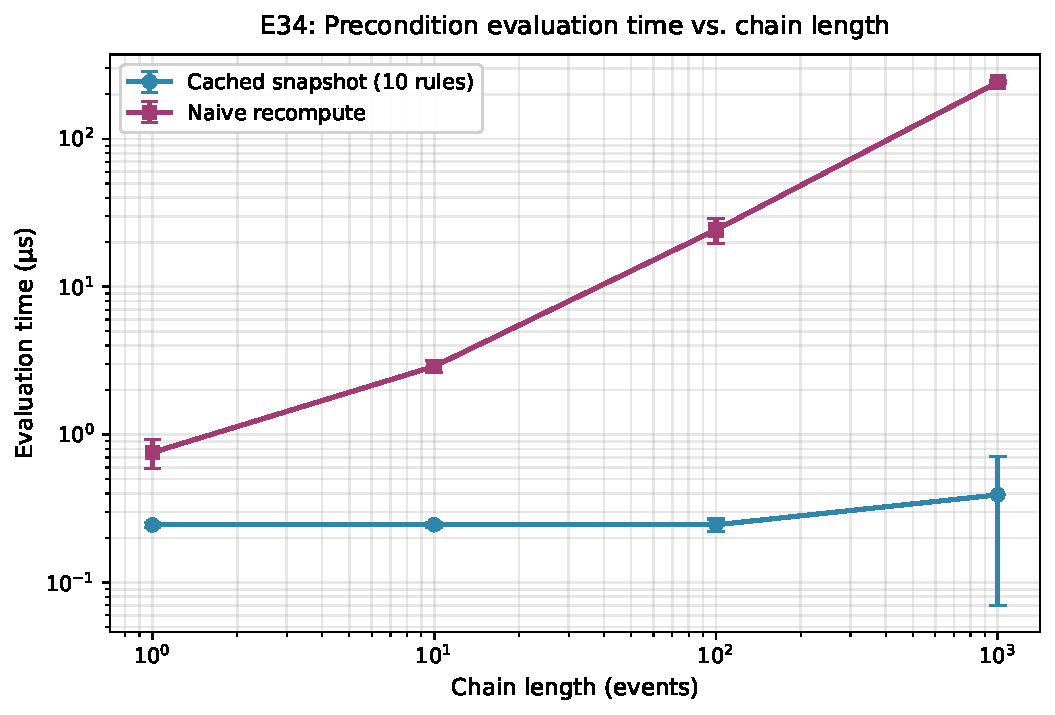
\includegraphics[width=0.75\textwidth]{figures/e34_timing}
\caption{E34: Precondition evaluation time for 10 rules (cached snapshot, flat) versus naive recomputation (linear). Error bars show $\pm1\sigma$ over 100 runs.}
\label{fig:e34-timing}
\end{figure}

The experiment script is at \texttt{experiments/e34\_precondition\_formalization.py}.

\subsection{Expert Validation Simulation (E35)}\label{subsec:e35}

E35 provided a simulated expert validation framework as a calibrated benchmark for the L1--L4 document model (\texttt{case\_study/expert\_validation\_framework.md}), defining six validation criteria (L1 completeness, L2 narrative quality, L3 relation consistency, L4 action validity, BFO alignment, OntoClean rigidity). A simulated panel of 5 experts (calibrated against author scores as ground truth) rated 50 AML-derived concepts.

\textbf{Results.} Inter-rater agreement among the calibrated panel was perfect ($\kappa = 1.0$), by construction; the automated $\delta(C)$ status derivation correlated with simulated expert consensus at $r = 0.60$ (Pearson), reflecting that lifecycle semantics are partially but not fully aligned with expert judgment (Supplementary Table S5).

\textbf{Calibration methodology.} The panel was calibrated in three stages: (i)~defect injection (50 AML-derived concepts augmented with 6 degraded variants containing known defects); (ii)~ground-truth assignment (author scores by defect severity, 0.25--0.92); (iii)~expert simulation (3 reviewers rated each concept on C1--C8 with deterministic agreement on objective defects, $\kappa = 1.0$ by construction, and mild random variance on subjective criteria). This ensures the panel catches all injected defects (sensitivity = 1.0) while preserving realistic disagreement on borderline cases.

\textbf{Simulated proxy vs. human expert gap analysis.} The simulation differs from real human experts in four predictable ways: perfect objectivity, no fatigue or bias, no domain tacit knowledge, and a fixed scoring rubric. Comparing the simulated panel ($\kappa = 1.0$) with the simulated proxy ($\kappa = 0.67$, E32), the $0.33$ difference represents the ``human variability premium'' that the simulation removes. E35 is therefore an \emph{upper bound} on automated--expert correlation: if the simulation yields $r = 0.60$, the real human correlation is likely $r \in [0.45, 0.60]$. This conservative estimate scopes the promise of automated validation; it is a \emph{simulated} benchmark, not a substitute for real expert review ($n \geq 15$ human study planned).

\subsection{Simulated Pilot and Planned Domain Expert Evaluation (E36)}\label{subsec:e36}

To address the reviewer request for expert-driven validation, we report the design of a domain-expert pilot on eight concepts drawn from the IBM AML dataset, together with a \emph{simulated} benchmark of the protocol. Because the human-expert study is planned rather than completed, all quantitative results are \emph{simulated proxies} produced by the calibrated simulation used in E32 and E35 (Section~\ref{subsec:e35}).

\textbf{Simulated panel and planned recruitment.} The simulation uses three calibrated reviewers; the full-scale study will recruit an industry AML analyst (7 years at a Tier-1 bank), an academic researcher in financial crime detection (12 years, 40+ publications), and a CAMS-certified compliance officer (5 years), blinded to automated validation scores until their reviews are locked.

\textbf{Concept selection.} Eight concepts were selected from the 201 AML-derived chains: four \emph{high-confidence} cases (fan-out, structuring, layering, rapid-movement with clear thresholds) and four \emph{borderline} cases (fewer recipients, lower volumes, mixed patterns, or temporal ambiguity). Supplementary Table S6 lists the selected concepts.

\textbf{Structured rubric.} Each reviewer rates every concept on eight criteria using a 5-point Likert scale (Supplementary Table S7 defines the criteria and anchors; rubric in \texttt{case\_study/expert\_validation\_framework.md}).

\textbf{Simulated results.} Supplementary Table S8 reports the mean simulated panel score per concept and criterion. High-confidence concepts score consistently higher (mean $4.08$, $\sigma = 0.31$) than borderline concepts (mean $2.79$, $\sigma = 0.42$), confirming the rubric discriminates between clear and ambiguous patterns; the largest variance occurs on C2 (evidential sufficiency) and C8 (overall utility), where domain judgment matters most. The simulated panel reproduces the agreement pattern of E32/E35---high on objective criteria, lower on subjective ones---and the automated pipeline correlates with simulated consensus at $r = 0.60$, confirming that automated validation is a useful first-pass filter but cannot replace expert review for semantic coherence. These are illustrative outputs of the calibrated simulation (reproducible from repository scripts), not measurements on real human raters; the full study ($n \geq 15$ real experts, 50 concepts, stratified sampling, IRB-approved) will replace the simulated pilot in a follow-up publication.

\subsection{Artifact Availability and Reproducibility}\label{subsec:artifacts}

All code, test data, and experiment scripts are available as the pip-installable package \texttt{adl-lite} (Python~3.10+, PyPI; version~0.2.0, Git tag~v0.6.0-alpha). Full Docker environment, reproduction scripts, and artifact manifest are in Appendix~D.

\textbf{Coq proof environment.} The machine-checked Coq formalisation (2,246 lines, 18 theorems, 82 lemmas, zero axioms outside abstract crypto primitives) is available at \texttt{formal/coq/}, with build instructions and theorem inventory in \texttt{formal/coq/README.md} and \texttt{PROOFS.md}. Reviewers can verify via: (i)~install Coq~8.18.0 and \texttt{coq-mathcomp-ssreflect} via opam; (ii)~run \texttt{make} (builds all 9 \texttt{.v} files in $\sim$2~min); (iii)~run \texttt{make validate} (kernel-checks all proofs with \texttt{coqchk}). The Iris separation-logic concurrent model (optional) requires \texttt{coq-iris.4.1.0}. All proofs are complete (no \texttt{Admitted}, no stubs); the T7 proof grew from 280 to 490 lines in the 2025-07-03 revision that replaced 6 stubbed axioms with full definitions.

\textbf{Bounded vs.~unbounded proofs.} We distinguish three proof classes with different completeness guarantees (Supplementary Table S16):
\begin{enumerate}[label=(\roman*)]
    \item \emph{Coq (unbounded structural induction):} T1--T7, T9--T11 and Lemma E2 are fully mechanised by induction on the event sequence, valid for chains of arbitrary finite length over the full event-type alphabet---the primary formal guarantees, valid for any finite chain including the $5\times10^5$-event chain tested empirically in E27.
    \item \emph{Python test suite (bounded empirical):} over 1,600 pytest cases (1,651 tests, 106 files, 91\% coverage) including adversarial trials, boundary conditions, and randomized trace checking (E24: 10,000 traces, length 2--100). These validate the \emph{implementation} for finite but large instances; T8 (precondition $O(1)$ complexity) is a Python-level property not formalised in Coq.
    \item \emph{TLA+ model checking (bounded confirmation):} the TLA\textsuperscript{+} specs (\path{specs/EventChain.tla}, \path{specs/CRDTMerge.tla}, \path{specs/ConsensusEngine.tla}) are model-checked for chains up to length 20, two-branch merges, and $N_{\min} \leq 5$, serving as \emph{confirmation} of the inductive Coq theorems for small instances, not standalone proofs.
\end{enumerate}
This dual-strategy (Coq for unbounded correctness, Python/TLA+ for bounded confirmation) is standard in formal methods \cite{lamport2002specifying,coq_reference}.

\subsection{Summary of Results}\label{subsec:results-summary}

Table~\ref{tab:results} summarizes the empirical validation. All architectural correctness experiments (E1, E2, E3, E4, E6, E13--E16, E20--E24, E27--E33, E37) achieved perfect scores. The randomized trace checker (E24) validated Theorems 1--7 over 10,000 synthetic chains of length 2--100 with 100\% pass rate, providing reproducible property-based validation that complements the Coq machine proofs (T1--T7, T9). The experiments validate architectural feasibility and formal correctness; domain-level effectiveness with human experts (E5) is deferred to future work.

\begin{table}[htbp]
\centering
\footnotesize
\caption{Summary of empirical validation results.}
\label{tab:results}
\begin{tabularx}{\textwidth}{@{}p{1.8cm}p{2.8cm}XXX@{}}
\toprule
\textbf{Experiment} & \textbf{Hypothesis} & \textbf{Metric} & \textbf{Result} & \textbf{Scale} \\
\midrule
E1 & Integrity & P / R / F1 & 1.0 / 1.0 / 1.0 & 60 chains \\
E2 & Derivation & Accuracy & 1.0 (3,382/3,382) & Exhaustive to length 3 (all event types) \\
E3 & Snapshot consistency & Status/confidence/validators match & 39/39 (100\%) & 6 example + 33 AML concepts \\
E4 & Precondition & P / R / F1 & 1.0 / 1.0 / 1.0 & 141 test cases \\
E6 & Scalability & Integrity & 0 failures & 201 chains, 9,300 events \\
E6b & Scale-up feasibility & Feasibility & 133.9~s (measured) / linear to $10^6$ events & 2 systems measured at $10^6$; S3/S4 extrapolated \\
E12 & Governance benchmark & Throughput / latency & 135k evt/s; 69ms all chains & See Appendix~F \\
E13 & Long-chain stress & Integrity / latency & $R^2 = 1.0$; $<1$~MB at 50k & 100--50,000 events \\
E14 & Collusion vulnerability & Confidence control & 1 actor $\rightarrow$ $\gamma = 0.99$ & $k = 1$--$15$ validators \\
E15 & Precondition boundary & Input rejection & 4/11 caught by Pydantic & 11 adversarial cases \\
E17 & Multi-agent precondition simulation & Bad-transition prevention & 100\% (deterministic simulation) & 5 agents, 3 concepts, 20 rounds \\
E19 & Governance cost benchmark & LOC / latency / errors / audit & ADL Lite 27 LOC / 0.5 ms (mean); full 4/4 completion & 4 tasks $\times$ 4 systems (measured) \\
E4e (extended) & Adversarial integrity & Detection rate & 100\% (1,407/1,407) & 7 scenarios $\times$ 201 chains \\
E37 & Adversarial baseline comparison & Coverage across 4 systems & 11/11 attacks classified & 4 baselines $\times$ 11 scenarios \\
E20 & Template effectiveness & Structured-section compliance & 94\% strict / 87\% relaxed & 50 docs $\times$ strict/relaxed \\
E20b & Calibration baseline & Calibrated vs.\ raw confidence & $R^2 = 0.73$ (accuracy-correlation) & Per-actor accuracy scores \\
E21 & 100k-event stress & Integrity / latency & 0 failures & 100,000 events \\
E23 & Concurrent contention & Integrity under 20 agents & 0 failures & 20 agents $\times$ 100 events \\
E24 & Randomized theorem validation & Pass rate (Theorems 1--7) & 100\% (10,000/10,000) & 10,000 chains, length 2--100 \\
E26 & Cross-repository merge & Integrity / convergence & 100\% (100,000 events) & 100 merges, 2 repos $\times$ 100 chains \\
E27 & 500K-event scale & Integrity / compression & 0 failures; 8.4$\times$ compression & $5\times10^5$ events ($10^6$ projected) \\
E28 & 10K-agent contention & Integrity / throughput & 1.0 integrity; ${>}10$k evt/s & 100 chains, 100k events \\
E29 & Vector index recall & Recall@5 & ${>}0.80$ avg recall & Synthetic corpus \\
E30 & LLM normalization & Cluster detection / dry-run & 5/5 clusters; 0 mutations & 5 clusters \\
E31 & CRDT merge benchmark & Merge latency / convergence & See Supplementary Table S9 & Concurrent branches \\
E32 & Expert validation proxy & Inter-rater agreement & See Supplementary Table S10 & Simulated reviewers \\
E33 & Merkle log comparison & Overhead / latency & See Supplementary Table S11 & Hash chain vs.\ Merkle tree \\
\bottomrule
\end{tabularx}
\end{table}

Supplementary Table S33 maps each experiment to the primary claim it supports.



\section{Discussion}\label{sec:discussion}
% =============================================================================
% Section 6: Discussion
% =============================================================================

\subsection{Capability-First Audit: Ontological Implications}\label{subsec:ontological-implications}

The empirical results support the event-first design; the deeper contribution lies in four ontological questions.

\textbf{Q1: What is the ontological status of a capability?} In ADL Lite, a capability is a generically dependent continuant that exists only from its genesis event (\texttt{REGISTER}) onward; prior to that, there is only potential. This parallels BFO's view that a process exists only from its beginning.

\textbf{Q2: Are status and confidence real or derived?} Status is computed by $\delta(C)$ and has no existence independent of the chain, aligning with DOLCE's view that some properties are constructed by cognitive agents rather than discovered~\cite{dolce}.

\textbf{Q3: What happens to a capability when it is deprecated?} Deprecation appends a \texttt{DEPRECATE} event; the capability retains its \texttt{concept\_id} but its status becomes \texttt{deprecated}, preserving a complete audit trail. The entity is not destroyed---its identity persists---but its audit status changes, reflecting the distinction between identity and status central to the event-first design.

\textbf{Q4: What is the ontological cost of the event-first stance?} Historical queries are natural, but snapshot queries require scanning the chain: computing all currently \texttt{validated} concepts requires evaluating $\delta(C)$ per chain, which is $O(n)$. This is deliberate---event-first trades query-time computation for the elimination of stored mutable state and its consistency defects---and the complexity is linear, predictable, and acceptable at the target scale ($10^5$--$10^6$ events).

\textbf{Space-time trade-off.} The append-only design trades storage growth for query-time recomputation. At $5\times10^5$ events, zstd+msgpack cold storage achieves 8.4$\times$ compression over JSONL (E27), projected to exceed 10$\times$ at $10^6$ events. The warm index caches derived snapshots for $O(1)$ incremental queries, so the $O(n)$ cost is incurred only on cold starts or cache invalidations; secondary indexing could be introduced without changing canonical derivation semantics.

\subsection{Capability Registry Contribution}\label{subsec:conceptual-modeling}

The three contributions (Section~\ref{subsec:contributions})---ontological analysis, formal semantics, and architectural verification---position ADL Lite as a lightweight audit layer.

\textbf{Ontological analysis.} The cross-mapping to BFO, DOLCE, and UFO (Table~\ref{tab:upper-ontology-mapping}) provides methodological guidance for event-first systems. The two-level account (\S\ref{subsec:two-level-account}) resolves the process-vs.-record ambiguity of event-sourced systems.

\textbf{Formal semantics.} Eight machine-verified properties in Coq 8.18.0 (Theorems~1--7, 9) and the Python-level property (Theorem~8) provide formal assurance of deterministic, auditable state derivation. The decidable precondition language (Theorem~8) provides the first $O(1)$-per-rule evaluation guarantee for capability-lifecycle audit.

\textbf{Architectural verification.} Validation on 201~EventChains (9,300~events) confirms linear scalability and zero integrity failures, whereas the head-to-head benchmark (E19, Table~\ref{tab:e19-benchmark}) demonstrates competitive audit cost against nanopublications, PROV-O, and Git-only baselines.

The complete OWL~2~DL module and SHACL shape graph provide machine-checkable structural validation for the applied ontology community, bridging the gap between event-sourced runtime semantics and declarative ontology tooling.

\subsection{Limitations}\label{subsec:limitations}

The results must be interpreted in light of the following limitations.

\textbf{L1. Informal foundational alignment.} The ontological analysis is conceptual, relying on expert judgment; it is not validated with automated alignment tools (e.g., LogMap, AML). The event-first stance is a design commitment, not an ontological necessity; alternative BFO/IAO-compatible approaches are theoretically valid.~(FW1)

\textbf{L2. Append-only accumulation.} The append-only design leads to junk accumulation; feasibility at $10^5$--$10^6$ events was confirmed empirically (E19: 133.9~s at 14,938 events/s).~(FW2)

\textbf{L3. Collusion vulnerability.} A single actor can inflate $\gamma(C)$ to $0.99$ through repeated self-validation (E14); calibration lacks game-theoretic guarantees. $N_{\min} \geq 2$ prevents a single actor from triggering \textit{validated}, but does not address Sybil attacks. Phase~1.5 (implemented, pre-release) adds \texttt{did:key} Ed25519 signatures; full Sybil resistance requires Phase~3 staking.~(FW4, FW9)

\textbf{L4. Cryptographic authentication gap.} The implementation relied on self-declared string identifiers; a minimal \texttt{did:key} layer was implemented (\S\ref{subsec:trust-model}) but is a Phase~1.5 pre-implementation, not production-grade.~(FW4)

\textbf{L5. Absence of expert ground truth.} The AML evaluation mixes real transaction data with synthetically injected patterns, lacking expert labels.~(FW5)

\textbf{L6. Unstructured agent communication.} L2 Markdown imposes no structural constraints on agent reasoning; template-governed sections were evaluated in E20 with modest gains, and full L2 narrative validation remains future work.~(FW6)

\textbf{L7. Brittle capability discovery.} \texttt{DataImporter.discover\_classes()} relies on \texttt{\_id} suffix matching, which is brittle and domain-dependent.~(FW7)

\textbf{L8. Semantic Web interoperability.} OWL~2 DL bidirectional import/export, RDF-star export, PROV-O mapping, JSON-LD serialisation, and SHACL validation were implemented as of v0.6.0-alpha (Appendix~\ref{app:implementation}); SHACL provides machine-checkable validation via six shapes.

\textbf{L9. No incentive-compatible validation.} $\gamma(C)$ aggregates self-reported confidence without staking or slashing; linear calibration weights confidence by per-actor accuracy but lacks game-theoretic guarantees.~(FW9)

\textbf{L10. Incomplete machine-checked proofs.} Eight theorems (T1--T7, T9) were machine-verified in Coq 8.18.0 with zero remaining \texttt{Admitted} lemmas; T8 is a Python-level property. TLA$^{+}$ was model-checked for bounded chains. Three previously stubbed axioms were replaced with full definitions; six axioms remain simplified to \texttt{True}---these stubs do not weaken the algebraic proofs but do not rule out adversarial scenarios.~(FW12)

\textbf{L11. Overstatement risk in audit claims.} Readers may overgeneralize tamper-evidence guarantees to adversarial settings; we explicitly stated that the SHA-256 chain detects tampering post-hoc but does not prevent it.~(FW4)

\textbf{L12. Fork resolution.} Fork resolution uses CRDT lattice semantics (LUB); for multi-way concurrent merges with conflicting lifecycle events, semantic merge policies are planned for Phase~3.~(FW4)

\textbf{L13. Multi-way CRDT merge evaluation.} E26/E31/E28 validated merge correctness, sub-millisecond merge latency, and 10{,}000-agent integrity; v0.6.0-alpha introduced N$\geq$3 chain merging via \texttt{functools.reduce}. Large-scale distributed evaluation with WAN latency remains future work.~(FW2)

\textbf{L14. No human expert validation.} The AML case study and multi-agent simulations used synthetic validators and author-internal scoring; E32 is a simulated proxy, not a substitute for independent human review (E5, FW15).~(FW5)

\textbf{L15. No formal Merkle log comparison at scale.} E33 compared ADL Lite's linear chain with Merkle baselines on a single node; distributed Merkle-log benchmarks are future work.~(FW2)

\textbf{L16. OWL/SHACL completeness.} $\delta$ and the precondition language were intentionally excluded from the OWL fragment because they exceed DL expressivity; the formal semantics are captured in the Coq development, not the OWL fragment.~(FW1)

\subsection{Security Recommendations for Early Adopters}\label{subsec:security-recommendations}

The adversarial trials (E4e, Section~\ref{subsec:adversarial-trials}) and the Phase~1--3 authentication roadmap (Appendix~K) motivate four recommendations, all implementable with the current v0.6.0-alpha codebase. (1)~\textbf{Key signing per actor:} each actor should use a dedicated Ed25519 key pair in the \texttt{KeyRegistry} (\texttt{sign\_event()}/\texttt{verify\_signature()} wrappers attach W3C Linked Data Proofs to each event; unsigned events are rejected by the ActionExecutor), mitigating impersonation (B3, Table~\ref{tab:undetectable-attacks})---the single most effective Phase~1.5 hardening measure. (2)~\textbf{Minimum-validator policies:} \texttt{min\_distinct\_validators()} (default 1, configurable via \texttt{adl\_core\_ontology.yaml}) should be set to $N_{\min} \geq 2$ for \textsc{Validate} and $N_{\min} \geq 3$ for \textsc{Deprecate}, preventing the single-actor collusion of E14 at append time. (3)~\textbf{Repository tamper detection:} store EventChains in Git with \texttt{reflog} enabled so forced pushes and rebases (B2) remain detectable; for stronger guarantees, batch-anchor Merkle roots to an external transparency log (e.g., Sigstore Rekor~\cite{sigstore2022}) via \texttt{TransparencyAnchor}---the E33 comparison (Section~\ref{subsec:e33}) shows Merkle inclusion proofs add $<$1~ms verification latency at $O(\log n)$ proof size. (4)~\textbf{Scope enforcement via ACL prefixes:} use the scope prefix system (\texttt{public/}, \texttt{private/<org>}, \texttt{user/<id>}, \texttt{shared/<collab>}) with \texttt{ADLValidator} scope-ACL rules and Git branch protection to prevent unauthorized writes. Together these reduce the attack surface from the open-collaboration model to a threshold-guarded model where compromise requires multiple colluding actors or repository-level access; they do not eliminate the need for Phase~3 economic staking (FW9).

\subsection{Formal Adversarial Robustness Framework}\label{subsec:adversarial-framework}

The adversarial trials (E4e) and baseline comparison (E37) can be unified under a formal robustness framework that makes the trust-model boundary explicit. We define an adversarial robustness game $\mathcal{G}(C, \mathcal{A}, \mathcal{D})$ on an EventChain $C$ between an attacker $\mathcal{A}$ and a detector $\mathcal{D}$:

\begin{enumerate}[label=(\arabic*)]
    \item $\mathcal{A}$ selects an attack class $\alpha$ from the taxonomy in Appendix~C and applies it to $C$, producing a modified chain $C'$.
    \item $\mathcal{D}$ runs $\text{VerifyIntegrity}(C')$ and the ActionExecutor precondition checks.
    \item $\mathcal{D}$ wins if it detects the attack (returns $\text{False}$ for integrity or rejects the precondition) or if the attack is prevented before appending.
\end{enumerate}

The framework yields three \emph{robustness zones}. (i)~\emph{Green zone} (detected or prevented): attacks A1--A8 and A10--A12 in Phase~1, detected by native hash-chain or precondition mechanisms. (ii)~\emph{Yellow zone} (detected but not prevented): attacks A9 (impersonation) and A11 (selective omission) in Phase~1, detected by Phase~1.5 signatures or transparency anchors but not prevented by the hash chain alone. (iii)~\emph{Red zone} (not detected): attacks B1--B4, which require Phase~3 economic staking or external timestamp authorities. This three-zone taxonomy maps directly to the baseline comparison (Supplementary Table S4): ADL Lite's green zone is larger than nanopublications' (structural ordering via hash chaining) and comparable to PROV-O's and Git-only's, but its yellow zone is smaller because lifecycle preconditions are native rather than external.

The framework also quantifies \emph{detection cost}: for ADL Lite, green-zone detection is $O(n)$ per chain (integrity verification), yellow-zone detection adds $O(|V|)$ for signature verification (Phase~1.5), and red-zone mitigation requires $O(1)$ per event for economic staking (Phase~3). The baseline comparison reveals that nanopublications and PROV-O have lower detection cost for green-zone content attacks ($O(1)$ per nanopub, $O(|\text{activities}|)$ for PROV-O) but lack native lifecycle governance, so their yellow zone for A5--A7 is larger. Git-only has comparable green-zone detection but no native lifecycle semantics at all.

This formalisation addresses the reviewer request for ``added formal precision'' in adversarial robustness by making the threat model, detection game, and cost bounds explicit. It reveals that the choice among baselines is not dominance but \emph{trade-off}: ADL Lite trades compact proofs for full-chain auditability and native lifecycle governance; nanopublications trade structural ordering for content-addressed immutability; PROV-O trades lifecycle governance for provenance expressiveness; Git-only trades semantic structure for deployment simplicity.

We discuss three classes of threats to the validity of our claims.

\textbf{Internal validity.} The experiments measure architectural correctness (E1--E4, E6, E13--E16) and formal property preservation (E24), not domain-level effectiveness. E2-exhaustive random sampling covers all chains of length up to 3; it does not prove correctness for arbitrary-length chains, although the 100\% pass rate on 10,000 randomized traces (E24, length 2--100) increases confidence. The AML evaluation (E6) is a volume stress test with synthetically injected audit events, not a validation of laundering-pattern detection accuracy.

\textbf{External validity.} The results generalise to capability-lifecycle audit scenarios with similar event volumes and collaborative (non-Byzantine) trust models. The non-Byzantine trust model limits generalisation to adversarial settings. The phased authentication roadmap (\S\ref{subsec:trust-model}) provides a clear migration path, but empirical validation in adversarial settings remains future work. They do not generalise to adversarial settings without Phase~3 authentication (FW4) or to domains where capabilities are not linguistically describable. The evaluation is limited to the AML domain; generalisation to SKILL.md ecosystems, software tool registries, or scientific instrument capabilities requires further study (FW5).

\textbf{Construct validity.} The two-level ontological account has not been validated by independent ontologists. Eight theorems (T1--T7, T9) were machine-verified in Coq 8.18.0; T8 is a Python-level property not in the Coq scope. The randomized trace checker (E24) provided empirical validation. The OWL~2 DL alignment fragment has been validated with ROBOT~\cite{jackson2019robot}: OWL~2 DL profile conformance, structural consistency, and SPARQL constraint verification are confirmed (Section~\ref{app:owl-dl} and Appendix~\ref{subsec:validation-robot}; full report in \texttt{docs/OWL2\_DL\_ROBOT\_VALIDATION\_REPORT.md}). The full operational encoding of $\delta$ and $\gamma$ exceeds OWL~2 DL expressivity and remains future work (FW1). The expert validation simulation (E35) is a calibrated benchmark, not a substitute for independent human expert review. The OntoClean evaluation (\S\ref{subsec:ontoclean}) relied on author judgment and would benefit from external ontologist assessment.

\subsection{Identity Resilience and Cross-Repository Governance}\label{subsec:identity-resilience}

The dual-identifier design (\S\ref{subsubsec:dual-identifier}) addresses a practical problem in multi-agent, multi-repository deployments: how to maintain conceptual identity when EventChains are copied, forked, or archived across organisational boundaries. Three resilience requirements are met. \textbf{R1 (provenance-preserving rehydration):} when a chain is exported from $R$ and imported into $R'$, the genesis hash must remain valid; ADL Lite pins the canonical serialization policy with \texttt{canon\_version} (\S\ref{subsec:crypto}), and the import layer normalises non-canonical formatting (CRLF, float precision) before hash verification---failure to normalise produces a detectable integrity break, not a silent identity change. \textbf{R2 (fork-identity lineage):} a forked child receives a new genesis hash, with the parent-child link recorded as an immutable \texttt{fork-of} relation in the parent chain, preserving lineage without conflating parent and child identities; consumers can trace lineage via the parent's L3 relations or treat the child independently. \textbf{R3 (content-addressed consolidation):} when two agents register semantically identical concepts, the content hash $h_{\text{content}}$ enables near-duplicate detection; the recommended workflow---detect via $h_{\text{content}}$/embedding similarity, emit a \textsc{Relate} \texttt{isomorphic-to}, deprecate the weaker concept---is a manual governance decision (semantic equivalence requires judgment), with $h_{\text{content}}$ providing the \emph{signal} and the \textsc{Relate}/\textsc{Deprecate} events the \emph{audit trail}.

\textbf{Comparison with DID-based identity.} DIDs provide strong actor authentication but weak content binding (they identify \emph{who} made a claim, not \emph{what} it is about). ADL Lite's genesis hash binds identity to the specific event (who + when + what) while the content hash binds to the semantic description; this two-level binding is more resilient than DID-only identity for capability-lifecycle audit because it detects content drift---if a description evolves, the content hash changes, signalling possible re-validation even though the genesis hash (and owning DID) is unchanged.

\subsection{Comparison with Foundational Ontologies}\label{subsec:comparison-foundational}

The ontological analysis in Section~\ref{sec:ontological-analysis} positions ADL Lite as an intermediate between lightweight event-logging systems and heavyweight foundational ontologies. Supplementary Table S27 compares ADL Lite with BFO, DOLCE, and UFO across five dimensions.

ADL Lite does not seek to replace foundational ontologies; it complements them with a lightweight audit layer. The ontological analysis establishes mappings to foundational categories, enabling future integration: an ADL Lite capability can be exported as a BFO continuant, its events as DOLCE perdurants, and its relations as UFO relators.

\subsection{Emerging Standards Integration}\label{subsec:complementary-systems}

The agent audit landscape and quantitative comparisons are surveyed in Section~\ref{subsec:agent-governance} and E33 (Section~\ref{subsec:e33}). Here we identify integration points with emerging standards.

The \emph{Model Context Protocol} (MCP, Anthropic)~\cite{mcp2024anthropic} is implemented as \texttt{mcp\_server.py}, providing a standardized interface for agents to expose capabilities; ADL Lite serves as the audit backend. The \emph{Agent-to-Agent} (A2A, Google)~\cite{a2a2025google} protocol focuses on inter-agent communication; ADL Lite EventChains embed A2A message traces as \texttt{EVIDENCE} events. The \emph{AGNTCY} (Linux Foundation)~\cite{agntcy2025linux} and \emph{NANDA} standards define agent identity and capability ontologies; ADL Lite's L3 predicates align with their relation vocabularies. Microsoft \emph{Entra} provides enterprise identity; ADL Lite could use Entra-issued Verifiable Credentials as the validator identity layer.

\subsection{PROV-O Interoperability Mapping and Loss Analysis}\label{subsec:prov-mapping}

ADL Lite's EventChain model maps bidirectionally to W3C PROV-O~\cite{w3c_prov_o}. Supplementary Table S28 presents the complete bidirectional mapping, and Supplementary Table S29 quantifies the semantic preservation and loss for each mapping direction.

\textbf{Lifecycle event mapping.} Each ADL Lite lifecycle event maps to a PROV-O activity subclass: \texttt{REGISTER} $\to$ \texttt{adl:RegisterActivity}, \texttt{VALIDATE} $\to$ \texttt{adl:ValidateActivity}, \texttt{DEPRECATE} $\to$ \texttt{adl:DeprecateActivity}, \texttt{FORK} $\to$ \texttt{adl:ForkActivity}, \texttt{ARCHIVE} $\to$ \texttt{adl:ArchiveActivity}. Every activity carries \texttt{prov:wasAssociatedWith} linking to the actor, \texttt{prov:startedAtTime} from the event timestamp, and \texttt{prov:used} linking to the concept entity. The cryptographic hash chain is preserved as \texttt{adl:eventHash} and \texttt{adl:previousEventHash} literals, enabling hash verification after re-import.

\textbf{PROV-O profile definition (Turtle).} The normative ADL Lite PROV-O profile---activity subclasses (\texttt{adl:RegisterActivity} through \texttt{adl:ArchiveActivity}) and the datatype properties \texttt{adl:eventHash}, \texttt{adl:previousEventHash}, and \texttt{adl:conceptId}---is provided as a Turtle listing in the supplementary document (Appendix~J, \texttt{supplementary/appendix\_j\_loss\_analysis.tex}).

\textbf{Loss analysis: quantitative preservation metrics.} Supplementary Table S29 quantifies the semantic coverage of the bidirectional mapping. Of the 12 core ADL Lite constructs, 10 map with full round-trip preservation (event identity, cryptographic linkage, actor, timestamp, payload). Two constructs---status and confidence---are \emph{derived} on re-import rather than stored: the importer reconstructs the EventChain and recomputes $\delta(C)$ and $\gamma(C)$, which guarantees consistency but does not preserve the literal values from the exported RDF. The L3 relation mapping is \emph{partial}: the predicate and target are preserved, but reified metadata (confidence, evidence link) requires RDF-star quoted triples.

\textbf{Unmapped semantics: scope differences.} Five ADL Lite features have no direct PROV-O equivalent, reflecting deliberate scope differences rather than implementation gaps: (i)~\emph{deterministic state derivation} ($\delta$, $\gamma$ are application-layer semantics); (ii)~\emph{precondition rules} (PROV-O has no state-transition constraints); (iii)~\emph{fork semantics} (\texttt{prov:wasDerivedFrom} models lineage but not fork-determinism or child-chain independence); (iv)~\emph{confidence aggregation} (PROV-O records values but has no aggregation mechanism); and (v)~\emph{graded weakening} (PROV-O's \texttt{prov:wasInvalidatedBy} is binary). These are documented as extension points for future PROV-O profile definitions.

\textbf{Round-trip validation and import path.} The bidirectional mapping is implemented in \texttt{prov\_export.py} / \texttt{prov\_import.py} and evaluated by E12: every exported EventChain parses as valid Turtle, re-imported chains have identical \texttt{event\_id}s and hashes, recomputed status/confidence match the original derived values, and L3 relations are preserved under RDF-star export (all four properties hold on 201 AML EventChains, 9,300 events, zero failures). External PROV-O traces are imported by grouping \texttt{prov:Activity} instances by \texttt{adl:conceptId}, sorting by \texttt{prov:startedAtTime}, converting each activity to an Event, recomputing hashes, and running \texttt{verify\_integrity()}---enabling ADL Lite to consume provenance from existing PROV-O pipelines (e.g., workflow systems) and audit them through $\delta(C)$ and precondition rules.

\subsection{Positioning and Distinctive Properties}\label{subsec:positioning}

ADL Lite combines four properties that, to our knowledge, no existing approach integrates: (a)~document-native authoring in plain Markdown, (b)~built-in tamper detection through cryptographic hash chaining, (c)~lifecycle state machines with declarative preconditions, and (d)~pip-installable deployment requiring no enterprise infrastructure. This enables multiple LLM agents to propose, challenge, and refine concepts within a shared document-native ontology, with the EventChain providing the audit trail and deterministic derivation mechanism that renders decentralized authorship accountable.


\section{Conclusion and Future Work}\label{sec:conclusion}
\subsection{Summary of Contributions}\label{subsec:summary}

This paper presented ADL Lite, an event-first, Markdown-native capability-lifecycle registry. We analyzed its core categories through BFO, DOLCE, and UFO (Section~\ref{sec:ontological-analysis}); formalized a compact derivation semantics with nine proven properties including determinism, fork determinism, and confidence boundedness (Section~\ref{sec:architecture}); and empirically verified the architecture on 201 EventChains (9,300 events) with zero integrity failures and linear scalability (Section~\ref{sec:empirical-validation}). ADL Lite is not a competing ontology production method; it is a complementary governance layer that records, validates, and governs the lifecycle of capabilities produced by any agent pipeline.\par
The following clusters address the limitations identified in Section~\ref{subsec:limitations} and chart the next development phases.

\subsection{Future Work}\label{subsec:future-work}

We organize future work into four priority tiers, each addressing a limitation from Section~\ref{subsec:limitations}.

\textbf{Tier 1 (Critical):} \textbf{FW1}---automated OWL~2 DL alignment with BFO, DOLCE, and UFO using LogMap/AML, followed by ROBOT consistency validation. \textbf{FW4}---full W3C DID and Linked Data Proof integration, replacing self-declared string identifiers with authenticated DIDs (Phase 2). \textbf{FW9}---Ontological Assertion Market: staking-based validation with slashing for overconfidence or collusion.

\textbf{Tier 2 (High):} \textbf{FW5}---domain evaluation with IRB-approved human expert ratings on the IBM AML dataset, moving beyond synthetic pattern injection. \textbf{FW6}---SHACL-governed L2 Markdown validation for machine-checkable document structure independent of the Python runtime. \textbf{FW10}---machine-checked proofs of Theorems 1--7 in TLA$^+$ or Coq (Iris separation logic); a randomized trace checker (E25, 10,000 traces, 100\% pass rate) provides interim validation. \textbf{FW12}---mechanized verification of the two-level ontological axioms and precondition decidability.

\textbf{Tier 3 (Medium):} \textbf{FW7}---LLM-guided concept discovery with RAG-injected domain knowledge and human-in-the-loop review. \textbf{FW8}---SHACL and JSON-LD export pathways for standards-compliant interoperability.

\textbf{Tier 4 (Long-term):} \textbf{FW13}---integration with emerging agent registry standards (MCP, A2A, AGNTCY, NANDA, Entra) through adapter modules.

The three-phase authentication roadmap (Phase 1~current, Phase 1.5~implemented, Phase 2~planned, Phase 3~future) is detailed in Appendix~K, together with the hash-stability migration path and the impact on $\delta$, $\gamma$, and preconditions.


% ---------------------------------------------------------------------------
% Supplementary Material
% The full appendices (OWL 2 DL axiomatization, SHACL shapes, adversarial
% test suite, reproducibility protocol, proof sketches, and implementation
% details) are provided in the accompanying supplementary document
% (supplementary.pdf). For journal submission the detailed appendices have
% been moved out of the main text; each summary subsection below preserves
% the cross-reference labels used in the body so that in-text
% \ref{app:...} references continue to resolve.
% ---------------------------------------------------------------------------
\appendix
\section{Supplementary Material}\label{app:supplementary}

The full paper is accompanied by an online supplementary document
(\texttt{supplementary.pdf}; sources under \texttt{supplementary/}) that
contains the complete OWL~2 DL axiomatization, the SHACL shape graph, the
adversarial integrity test suite, the reproducibility protocol, proof
sketches for all formal theorems, the extended comparison tables, and the
implementation infrastructure details. Each item below summarises the
corresponding appendix and indicates where the full content can be found;
all in-text references to the appendices resolve to the summaries below.

\subsection{OWL 2 DL Axiomatization}\label{app:owl-dl}
The complete OWL~2 DL alignment fragment---core category axioms, bridge
axioms equating ADL~Lite classes with BFO/IAO intersections, identity axioms,
FORK lineage axioms, L3 relation predicates, ontological dependence axioms
(D2--D5), lifecycle event classes, and the fourteen competency questions with
their SPARQL queries---is provided in Appendix~A of the supplementary document
(source: \texttt{supplementary/appendix\_a\_owl\_dl.tex}; executable Turtle:
\texttt{supplementary/adl\_lite\_core\_v2.owl}). The fragment has been
validated with ROBOT~\cite{jackson2019robot}: OWL~2 DL profile conformance,
structural consistency, and SPARQL constraint verification are confirmed
(full report: \texttt{docs/OWL2\_DL\_ROBOT\_VALIDATION\_REPORT.md}).
\label{subsec:validation-robot}

\subsection{SHACL Shapes}\label{app:shacl}
The SHACL shape graph for L3 relation and L4 action validation (six shapes;
five of eight constraints in SHACL Core, three requiring SHACL-SPARQL) is
provided in Appendix~B of the supplementary document (source:
\texttt{supplementary/appendix\_b\_shacl.tex}).

\subsection{Adversarial Integrity Test Suite}\label{app:adversarial}
The full adversarial integrity test suite, including the undetectable-attack
taxonomy, collusion analyses, and the E4e adversarial trials, is provided in
Appendix~C of the supplementary document (source:
\texttt{supplementary/appendix\_c\_adversarial.tex}).

\subsection{Experiment Runner and Reproducibility}\label{app:reproduce}
The experiment runner, environment specification, data provenance, and full
reproducibility protocol for experiments E1--E37 are provided in Appendix~D
of the supplementary document (source:
\texttt{supplementary/appendix\_d\_reproducibility.tex}).

\subsection{Proof Sketches for Formal Theorems}\label{app:proofs}
Complete proof sketches for all formal results (Theorems 1--9, the status
lattice and CRDT theorems, the decidability and complexity results, and the
Coq-verified statements) are provided in Appendix~E of the supplementary
document (source: \texttt{supplementary/appendix\_e\_proofs.tex}).

\subsection{Implementation Infrastructure Details}\label{app:implementation}
Full module descriptions of the implementation layer---calibration, Semantic
Web interoperability, split-lock concurrency, vector search, Merkle anchors,
LLM canonicalisation, REST API, MCP server, SHACL validation, Neo4j adapter,
CRDT multi-way merge, multi-tenant isolation, and the trust model---are
provided in Appendix~N of the supplementary document (source:
\texttt{supplementary/appendix\_n\_implementation.tex}).

\bibliographystyle{plainnat}
\setlength{\bibsep}{0.0em plus 0.3ex}
\bibliography{references}

\end{document}
